\documentclass[10pt,twocolumn]{article}

\usepackage[utf8]{inputenc}
\usepackage[T1]{fontenc}
\usepackage{lmodern}
\usepackage{microtype}
\usepackage[margin=0.72in,top=0.8in,bottom=0.85in]{geometry}
\usepackage{amsmath,amssymb,amsfonts,amsthm,bm,mathtools}
\usepackage{graphicx}
\usepackage{booktabs}
\usepackage{multirow}
\usepackage{array}
\usepackage{xcolor}
\usepackage{hyperref}
\usepackage{algorithm}
\usepackage{algpseudocode}
\usepackage{enumitem}
\usepackage{caption}
\usepackage{subcaption}
\usepackage{cite}
\usepackage{fancyhdr}
\usepackage{placeins}
\usepackage[raggedright]{titlesec}

\definecolor{deepblue}{RGB}{0,90,160}
\definecolor{AlertRed}{RGB}{190,40,30}
\definecolor{ForestGreen}{RGB}{0,130,90}

\hypersetup{
    colorlinks=true,
    linkcolor=deepblue,
    citecolor=deepblue,
    urlcolor=deepblue,
    pdftitle={%
    Reliable Multimodal Biomedical Fusion Under Missing Modalities, Biomarker Discordance, and
    High-Dimensional Omics Redundancy via DeepFuzzyTorch},
    pdfauthor={Guanqun Sun}
}

\captionsetup{font=small,labelfont=bf}
\setlength{\columnsep}{0.24in}
\tolerance=2000
\emergencystretch=3.0em
\raggedbottom
\setcounter{dbltopnumber}{1}
\renewcommand{\dbltopfraction}{0.99}
\renewcommand{\textfraction}{0.01}
\renewcommand{\dblfloatpagefraction}{0.85}

\newtheorem{theorem}{Theorem}
\newtheorem{lemma}[theorem]{Lemma}
\newtheorem{proposition}[theorem]{Proposition}
\newtheorem{corollary}{Corollary}[theorem]
\newtheorem{definition}{Definition}
\newtheorem{remark}{Remark}

\pagestyle{fancy}
\fancyhf{}
\fancyhead[L]{\footnotesize \textit{Formatted in Nature Portfolio (Results-First) Style}}
\fancyhead[R]{\footnotesize \textit{DeepFuzzyTorch: Reliable Multimodal Biomedical AI Under
Missingness \& Conflict}}
\fancyfoot[C]{\footnotesize \thepage}
\renewcommand{\headrulewidth}{0.4pt}

\title{\vspace{-1.0em}%
\textbf{Reliable Multimodal Biomedical Fusion Under Missing Modalities, Cross-Modal Biomarker
Discordance, and High-Dimensional Omics Redundancy via \texttt{DeepFuzzyTorch}}}

\author{
\textbf{Guanqun Sun}\\
\small School of Medical Imaging and Artificial Intelligence, Hangzhou Medical College,
Hangzhou 310053, China\\
\small Open-Source PyTorch Operator Library \& Benchmark Suite:
\url{https://github.com/SUN-1024/DeepFuzzyTorch}
}

\date{}

\begin{document}

\maketitle

\begin{abstract}
Multimodal biomedical AI faces missing modalities, biomarker discordance, and opaque decisions.
We present \texttt{DeepFuzzyTorch}, a curated PyTorch integration of fuzzy fusion, rough
feature selection, interpretable rules, and test-time adaptation. Vacuity mapping guarantees
exact $0.00$ fixed-width padding invariance for unacquired slots. Across 5,356 participants and
4,849 pathology records, empirical benchmarks show ADNI Cohort~1 AUROC of $0.8270$ ($N=1,137$)
and $0.8371$ (complete $N_{\mathrm{comp}}=854$), missingness retention $\mathrm{MRR}=0.9344$,
60-month conversion AUROC $0.9419$, and OASIS-3 transfer AUROC $0.8639$. Observed conflict
detects swaps at $0.7000$ AUROC and is $1.51\times$ higher in discordant ADNI participants. A
20-gene TCGA reduct yields $0.7403$ versus $0.6925$ AUROC for the matched unreduced model.
\end{abstract}

\section{Introduction}
\label{sec:intro}

Modern clinical diagnostics and precision oncology rely on synthesizing complementary evidence
across heterogeneous biological scales \cite{baltrusaitis2018multimodal,acosta2022multimodal}.
In neurodegenerative diseases such as Alzheimer's disease (AD), revised criteria distinguish
Core~1 diagnostic AD biomarkers, including amyloid and phosphorylated tau measures, from
staging or non-specific injury markers such as FDG-PET and glial fibrillary acidic protein
(GFAP) \cite{jack2024revised,palmqvist2020discriminative,janelidze2020plasma}. Clinical
assessment can also include structural magnetic resonance imaging (MRI), plasma phosphorylated
tau-181 (pTau181), and neurocognitive scores. In computational oncology, prognostic
stratification combines gigapixel histopathology whole-slide images (WSIs) encoded by vision
foundation models \cite{chen2024uni,lu2024visual,filiot2023scaling,filiot2024phikonv2,%
kaiko2024towards,wang2022transformer,huang2023visual} with multi-omic molecular signatures and
clinical staging \cite{kather2019predicting,jaume2024survpath}. In a separate clinical setting,
MUSE learns multimodal graph representations of EHR and neuroimaging data \cite{wu2024muse}.

Despite the proliferation of multimodal deep learning architectures, translating these models
from curated research benchmarks into routine hospital workflows faces four fundamental
obstacles \cite{shaik2024survey,shao2024dual,yao2024drfuse,%
liang2021multibench}:
\begin{enumerate}[leftmargin=1.4em,itemsep=1pt,topsep=2pt]
    \item \textbf{Combinatorial Missing Modalities ($2^M-1$ Nonempty Subsets, Including $2^M-2$
    Incomplete Subsets):} Due to insurance constraints, radiation exposure limits, or assay
    availability, patients rarely possess all $M$ modalities at inference time
    \cite{wu2024muse,yao2024drfuse}. Standard early concatenation and cross-attention
    transformers \cite{vaswani2017attention,arevalo2017gated} rely on zero/mean imputation,
    attention key-padding masks, or generative synthesis \cite{ma2021smil}. However, feeding
    zero-imputed feature vectors into unmasked neural layers injects synthetic bias activations
    that masquerade as observed evidence, while standard attention masking does not decompose
    belief into directional support ($\mu$), refutation ($\nu$), and epistemic ignorance
    ($\pi$).
    \item \textbf{Cross-Modality Evidence Conflict \& Physiological Confounding:} Real-world
    modalities frequently contradict one another due to sensor artifacts or systemic
    comorbidities \cite{xu2024reliable,zhang2023provable}. Community studies associate chronic
    kidney disease (CKD) and lower estimated glomerular
    filtration rate (eGFR) with elevated plasma pTau181 and pTau217 concentrations
    \cite{mielke2022performance}; this association does not establish diagnostic confounding
    or its cause. Classical Dempster--Shafer combination rules suffer from
    Zadeh's paradox \cite{shafer1976mathematical,zadeh1986simple,denoeux2019decision}, where
    normalizing by $1-K$ under high conflict ($K\to 1$) concentrates belief masses rather than
    inflating epistemic abstention.
    \item \textbf{High-Dimensional Feature Redundancy and Boundary Ambiguity:} Regional brain
    morphometry (e.g., 320 Free\-Surfer cortical/subcortical features) and pan-cancer
    transcriptomics (1,000+ protein-coding genes) exhibit severe collinearity and overlapping
    class boundaries, causing overfitting or unstable sparse feature selection across folds
    \cite{peng2005feature,yamada2020feature,cui2021curse}.
    \item \textbf{Lack of Auditable White-Box Rule Heads \& Domain Shift Resilience:} Black-box
    fusion heads cannot export human-\allowbreak verifiable decision rules for clinical audit
    \cite{rudin2019stop}, and multi-expert foundation model ensembles degrade when an expert
    model is corrupted under cross-\allowbreak hospital or cross-\allowbreak cohort shifts
    \cite{wang2021tent}.
\end{enumerate}

Reconciling data-driven deep representation learning with axiomatic mathematical priors has
recently catalyzed domain-specific differentiable operator libraries in PyTorch
\cite{paszke2019pytorch}, including \texttt{Kornia} for differentiable geometric computer
vision \cite{riba2020kornia}, \texttt{Theseus} for nonlinear least-squares optimization
\cite{pineda2022theseus}, \texttt{PyPose} for Lie-group manifold learning
\cite{wang2023pypose}, and \texttt{LTNtorch} for differentiable real-valued first-order
fuzzy logic tensor networks \cite{badreddine2022ltntorch}. In granular uncertainty modeling,
classical fuzzy set theories \cite{zadeh1965fuzzy} provide mathematical structures tailored for
incomplete, conflicting, and ambiguous clinical evidence; however, existing software toolkits
and deep fuzzy fusion architectures have complementary strengths. The
\texttt{scikit-learn}-compatible \texttt{fuzzy-rough-learn} library
\cite{lenz2022fuzzyroughlearn} supports configurable ordered-weighted-average (OWA) soft
minima and maxima; \texttt{ChIMP}/\texttt{iChIMP} offers differentiable Choquet aggregation
of scalar source scores \cite{islam2020chimp}; and deep TSK classifiers provide rule networks
\cite{wu2020optimize,cui2021curse}. These tools do not combine PyTorch autograd with the
intuitionistic vacuity and conflict decomposition and offline permutation-calibrated selection
studied here. Specifically, Atanassov's
Intuitionistic Fuzzy Sets (IFS)
\cite{atanassov1986intuitionistic,xu2007intuitionistic} decompose belief into membership $\mu$,
non-membership $\nu$, and epistemic hesitancy $\pi = 1 - \mu - \nu$. Torra's Hesitant Fuzzy
Sets (HFS) \cite{torra2010hesitant,xia2011hesitant,xia2012entropy,liao2013vikor} capture
inter-expert dispersion. Pawlak--Dubois--Prade Fuzzy-Rough Sets (FRS)
\cite{pawlak1982rough,dubois1990rough,jensen2004fuzzy} formalize attribute dependency via lower
and upper approximations. Yager's Pythagorean Fuzzy Sets (PFS) \cite{yager2014pythagorean}
relax linear simplex constraints to $\mu^2 + \nu^2 \le 1$, and Takagi--Sugeno--Kang (TSK)
systems \cite{takagi1985fuzzy,jang1993anfis,wu2020optimize,cui2021curse} express nonlinear
inference through transparent \texttt{IF--THEN} rules. Yet integrating these five paradigms
end-to-end inside autograd pipelines has remained hindered by non-differentiable $\min/\max$
operators, $O(K_f^D)$ rule-base explosion, and floating-point cancellation near simplex
boundaries.

Prior multimodal and uncertainty-aware learning frameworks address only isolated facets of
these clinical failure modes (Supplementary Table~\ref{tab:paradigm_comparison}).
\label{sec:related}
Handling missing modalities at inference time has been approached through latent imputation and
cross-modal generation \cite{ma2021smil}, attention key-padding masks
\cite{vaswani2017attention,shaik2024survey}, and shared-specific representation
disentanglement in DrFuse \cite{yao2024drfuse}. Related multimodal methods address distinct
settings: MUSE learns clinical EHR/neuroimaging patient--modality graph representations
\cite{wu2024muse}; SurvPath performs pathway--histology survival fusion
\cite{jaume2024survpath}; EMMS uses non-generative evidential survival fusion
\cite{xing2026emms}; and FUML uses fuzzy possibility/necessity multi-view learning
\cite{duan2025fuml}. Generative synthesis \cite{ma2021smil} propagates reconstructed
activations through downstream layers, risking hallucination when key modalities are
unacquired, whereas shared-encoder transformers \cite{vaswani2017attention,yao2024drfuse} can
degrade when dominant clinical modalities drop out at test time. Non-generative evidential
survival fusion in EMMS \cite{xing2026emms} represents missing modalities as vacuous evidence
via Gaussian random fuzzy numbers, while FUML \cite{duan2025fuml} models view-specific fuzzy
possibility and necessity memberships on complete multi-view data.
As formalized in Methods (Section~\ref{sec:method}, Theorem~\ref{thm:degeneration} and
Corollary~\ref{cor:e2e_vacuity}), our framework extends exact
missing-modality invariance to Atanassov intuitionistic fuzzy Choquet aggregation and
concept-masked TSK inference: mapping an absent modality to $\mathcal{A}_{\text{miss}} =
\langle 0, 0, 1\rangle$ yields exact $0.00$ fixed-width padding deviation across standalone
fusion and the end-to-end multimodal pipeline (matching restricted variable-width submodels
within float32 reduction rounding $\le 10^{-7}$ in the Track-0 benchmark audit; tested
default-scale variable-width unit checks give $\le 10^{-6}$) without generative imputation.



Subjective Logic and Evidential Deep Learning (EDL)
\cite{sensoy2018evidential,han2022trusted,shao2024dual,xu2024reliable} parameterize Dirichlet
concentration parameters
$\bm{\alpha}$ or basic belief assignments to combine multi-view opinions. Quality-aware
Multimodal Fusion (the original QMF method; the comparator is QMF (adapted))
\cite{zhang2023provable} separately weights unimodal logits via energy-based
uncertainty and training-trajectory stability, while Reliable Conflictive Multi-View Learning
(RCML) \cite{xu2024reliable} explicitly models conflictive multi-view opinions via evidential
averaging. Dual-level deep evidential fusion (DDEF) \cite{shao2024dual} integrates multimodal
evidence at the BBA and modality levels, and ECoLaF \cite{deregnaucourt2025ecolaf} introduces
pixel-wise conflict-guided discounting with Dempster--Shafer combination to mitigate Zadeh's
normalization paradox \cite{zadeh1986simple}. While effective for evidential opinion pooling,
these architectures do not model non-additive coalition capacities across correlated clinical
modalities, fuzzy-rough boundary regions in high-dimensional tabular/transcriptomic spaces, or
white-box TSK rule extraction. \texttt{DeepFuzzyTorch} couples certainty-ordered
Choquet-style capacity integration \cite{choquet1954theory,xu2010choquet} with exponential
cross-polarity conflict discounting inside capacity-weighted geometric-hesitancy intuitionistic
aggregation. Its capacity weights depend on observed certainties and therefore do not define a
fixed-capacity Choquet integral. At fixed certainty $r_m$, the integration provably routes
inter-modality contradiction into epistemic hesitancy $\pi_{\text{fused}}$
(Theorem~\ref{thm:conflict}).



Classical fuzzy-rough attribute reduction
\cite{dubois1990rough,jensen2004fuzzy,cornelis2010attribute} includes hard $\inf/\sup$
extrema. The \texttt{scikit-learn} toolkit \texttt{fuzzy-rough-learn}
\cite{lenz2022fuzzyroughlearn} also supports configurable OWA soft minima and maxima.
\texttt{DeepFuzzyTorch} instead integrates \texttt{DifferentiableFuzzyRoughLayer} and the
unimodal \texttt{FuzzyRoughAttentionGate} with PyTorch autograd, alongside an offline
permutation-null-calibrated T-norm selector \texttt{FuzzyRoughFeatureReducer}. Related
selection strategies include neural stochastic gates \cite{yamada2020feature} and
mutual-information filters \cite{peng2005feature}. Meanwhile, PyTorch real-valued logic
libraries such as
\texttt{LTNtorch} \cite{badreddine2022ltntorch} ($[0,1]$ scalar truth predicates), explainable
Choquet integral neural fusion networks such as \texttt{ChIMP}/\texttt{iChIMP}
\cite{islam2020chimp} (aggregating real-valued source inputs via SGD without explicit
$(\mu,\nu,\pi)$ vacuity or conflict discounting), and high-dimensional TSK systems
\cite{jang1993anfis,wu2020optimize,cui2021curse} either lack intuitionistic/rough uncertainty
decomposition or face rule-base explosion on hundreds of raw features. Our framework integrates
a temperature-controlled soft-{\L}ukasiewicz operator preserving $\underline{R}_\tau(A) \le A
\le \overline{R}_\tau(A)$ alongside a MAD-standardized pointwise T-norm fuzzy-rough reducer
with permutation-null calibration (Theorem~\ref{thm:rough}) and a concept-masked TSK rule head.

To bridge this gap, we present \texttt{DeepFuzzyTorch}, an open-source curated integration of
existing axiomatic fuzzy primitives into a PyTorch operator library and multimodal framework
(Figure~\ref{fig:paradigm_teaser}).
Rather than claiming universal AUROC dominance over unconstrained black-box architectures when
all modalities are cleanly observed, \texttt{DeepFuzzyTorch} delivers competitive
discrimination on heterogeneous clinical cohorts while providing structural guarantees---exact
fixed-width
missing-modality vacuity invariance, conflict-driven hesitancy triage, stable in-fold feature
reduction, and machine-precision white-box rule export---unavailable in standard neural fusion.
Our main contributions are summarized as follows:

\begin{figure*}[t]
    \centering
    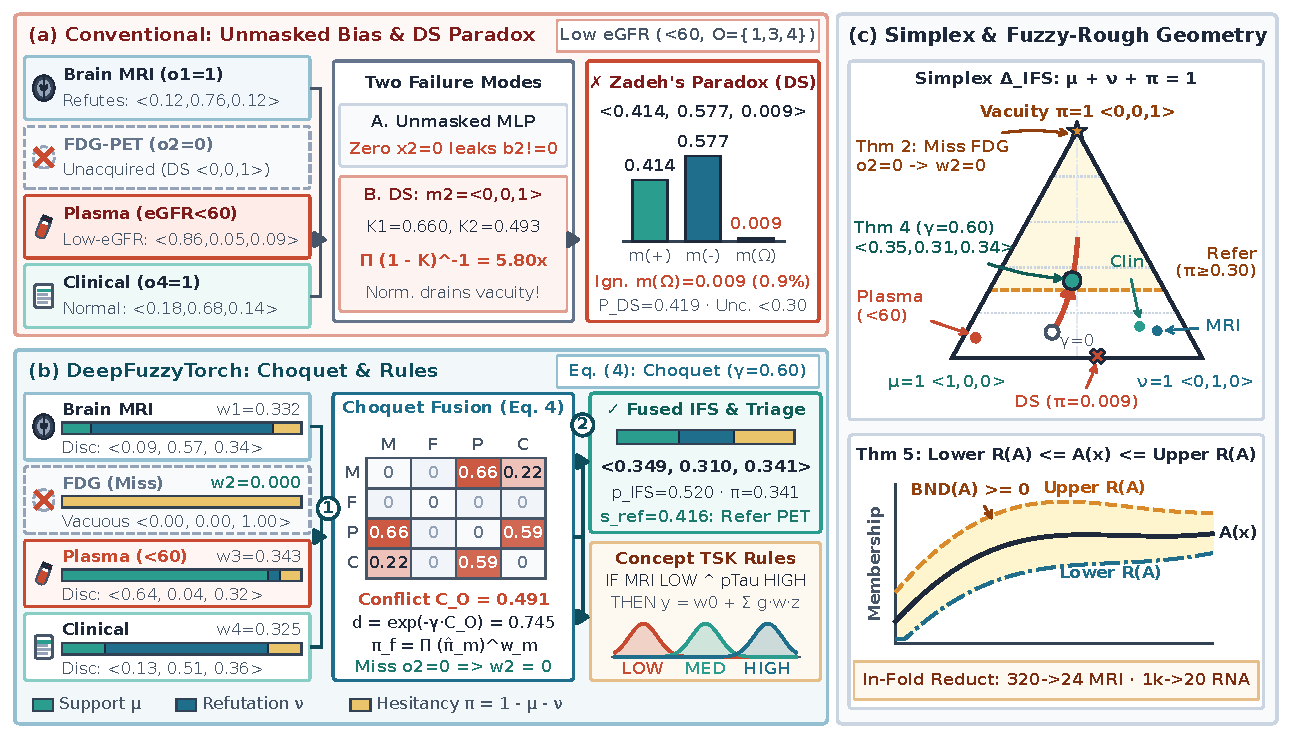
\includegraphics[width=\textwidth]{../figures/Fig0_Paradigm_Teaser_Comparison.pdf}
    \caption{\textbf{Conceptual and numerical walkthrough contrasting conventional multimodal
    fusion with \texttt{DeepFuzzyTorch}.} Illustrated on an amyloid-negative ($A\beta^-$)
    chronic kidney disease ($\text{CKD}$, $\text{eGFR}<60$) patient with observation indicator
    $\bm{o}_i=[1,0,1,1]$ ($\mathcal{O}_i=\{1,3,4\}$: observed MRI $\langle 0.12, 0.76,
    0.12\rangle$, unacquired FDG-PET, renal-confounded Plasma pTau $\langle 0.86, 0.05,
    0.09\rangle$, and Clinical $\langle 0.18, 0.68, 0.14\rangle$). \textbf{(a)} Conventional
    pipelines exhibit two distinct pitfalls: unmasked zero-imputation leaks affine layer bias
    ($W_2\cdot \mathbf{0}+b_2\neq 0$), whereas classical Dempster--Shafer fusion of observed
    modalities with vacuous missing FDG-PET ($m_2=\langle 0,0,1\rangle$) amplifies belief by
    $5.80\times$ and collapses ignorance from $0.117$ to $m_{\text{DS}}(\Omega)=0.009$
    ($99.1\%$ committed mass, $P_{\text{DS}}=0.419$, failing the $m(\Omega)\ge 0.30$ referral
    trigger). \textbf{(b,c)} \texttt{DeepFuzzyTorch} maps unacquired FDG-PET to exact vacuity
    $\langle 0, 0, 1\rangle$ ($w_2=0.0000$; Methods, Theorem~\ref{thm:degeneration}), detects
    active
    conflict $C_{\mathcal{O}}=0.491$ ($d=0.745$ at $\gamma=0.60$), inflates fused hesitancy to
    $\langle 0.349, 0.310, 0.341\rangle$ ($p_{\text{IFS}}=0.520$, Theorem~\ref{thm:conflict})
    to trigger selective PET referral ($s_{\text{ref}}=0.416$), and exports white-box
    \texttt{IF--THEN} rules.}
    \label{fig:paradigm_teaser}
\end{figure*}
\begin{itemize}[leftmargin=1.3em,itemsep=1pt,topsep=2pt]
    \item \textbf{Unified Differentiable Fuzzy-Rough Library:} We formulate five composable
    PyTorch operator modules anchored by our constrained simplex tensor abstraction
    (\texttt{Intuitionistic\allowbreak Fuzzy\allowbreak Tensor}): (1) \texttt{IFS\allowbreak
    Choquet\allowbreak Fusion}, (2) \texttt{Hesitant\allowbreak Fuzzy\allowbreak Aggregator},
    (3) \texttt{Differentiable\allowbreak Fuzzy\allowbreak Rough\allowbreak Layer} (paired with
    \texttt{FuzzyRough\allowbreak Feature\allowbreak Reducer} and \texttt{FuzzyRough\allowbreak
    AttentionGate}), (4) \texttt{Deep\allowbreak Concept\allowbreak TSK\allowbreak Head}, and
    (5) \texttt{Pythagorean\allowbreak Fuzzy\allowbreak TTA\allowbreak Loss}.
    \item \textbf{Theoretical Guarantees and End-to-End Verification:} In Methods
    (Section~\ref{sec:method}) and Supplementary Information (Appendix~\ref{app:proofs}), we
    prove and numerically verify five foundational properties and an end-to-end corollary.
    Specifically, we
    establish IFS simplex closure ($\le 5.96\times 10^{-8}$ float32 residual) and piecewise
    $C^\infty$ smoothness on fixed active sets $\mathcal{O}$ across strict certainty-ordering
    chambers (with fixed-$\mathcal{O}$ $C^0$ $\pi_{\text{fused}}$ continuity on
    $(\Delta_{\text{IFS}} \setminus \{\langle 0,0,1\rangle\})^{|\mathcal{O}|}$ across multiway
    positive-certainty tie blocks $B(r)$ in $\mathcal{H}_{\text{tie}}$, canonical index
    tie-breaking, and documented $\gamma$-independent conflict-denominator jumps in
    $C_{\mathcal{O}}$ alongside resulting $O(\gamma/|\mathcal{O}|)$ discount jumps at $\gamma >
    0$). We further prove exact $0.00\times 10^0$ fixed-width missing-modality vacuity
    invariance ($\langle 0,0,1\rangle$) and exact-arithmetic submodel equivalence within
    float32 rounding via binary concept masking $\bm{m}_{z,i}$ (Theorem~\ref{thm:degeneration}
    and Corollary~\ref{cor:e2e_vacuity}), strict partial-order monotonicity ($\ge 0.2072>0$,
    $5.20\times 10^{-8}$ analytic-vs-FD error), conflict-driven hesitancy inflation, and
    soft-{\L}ukasiewicz bound inclusion ($0.00\times 10^0$ violation) alongside
    MAD-standardized pointwise T-norm granular monotonicity.
    \item \textbf{Auditable Concept-Masked White-Box TSK Rule Export:} Our concept-bottleneck
    TSK head operates on $C \le 8$ masked clinical and modality net-support concepts,
    reconstructing Fold-0 validation logits within $2.84 \times 10^{-7}$ from structured
    float32 dictionaries and $2.384 \times 10^{-7}$ ($\le 2.39 \times 10^{-7}$) when parsed
    directly from human-readable 8-decimal \texttt{IF--THEN} text rules via
    \texttt{evaluate\_\allowbreak exported\_\allowbreak rules\_\allowbreak text()}.
    \item \textbf{Rigorous Multi-Center Validation Against Modern Baselines:} We benchmark
    across 5,356 unique clinical/oncology participants and 4,849 histopathology records against
    fourteen multimodal and tabular comparators---including \texttt{QMF (adapted)}
    \cite{zhang2023provable},
    multimodal adaptations of \texttt{RCML (adapted)} \cite{xu2024reliable},
    \texttt{DrFuse (adapted)}
    \cite{yao2024drfuse}, \texttt{DDEF (adapted)} \cite{shao2024dual}, and \texttt{FUML
    (adapted)}
    \cite{duan2025fuml}, \texttt{XGBoost} \cite{chen2016xgboost}, \texttt{CatBoost}
    \cite{prokhorenkova2018catboost}, \texttt{TabPFN~v2} \cite{hollmann2025tabpfn},
    equalized-supervision fairness controls, four transcriptomic feature selectors
    (\texttt{PCA-20}, \texttt{MI-20}, \texttt{Lasso-20}, \texttt{mRMR-20}), and
    \texttt{Logit-Tent (adapted)} from \texttt{Tent} \cite{wang2021tent}. Across six tracks, we
    separate ADNI Cohort~1 full-population ($N=1,137$, $0.8270$), same-visit ($n=924$,
    $0.8387$), and complete four-modality ($N_{\text{comp}}=854$, $0.8371$) metrics alongside
    superior tree/foundation-model missingness retention ($\text{MRR}=0.9344$), separated
    conflict detection ($0.7000$ pure $C_{\mathcal{O}}$ vs.\ $0.6542$ composite), strictly
    nested
    ADNI discordance ($N=1,112$, $p=1.75\times 10^{-17}$) with matched-coverage referral
    ($n=198$), longitudinal conversion ($0.9419$ AUROC), 5-seed OASIS-3 transfer ($0.8639\pm
    0.0010$), supervised in-fold TCGA RNA reduction with Reactome enrichment ($m=676$), and
    corrupted-expert pathology consensus.
\end{itemize}

Formal operator definitions and full statements of our five mathematical guarantees
(Theorems~\ref{thm:closure}--\ref{thm:rough} and Corollary~\ref{cor:e2e_vacuity}) are presented
in Methods (Section~\ref{sec:method}), with end-to-end forward inference pseudocode
(Supplementary Algorithm~\ref{alg:deepfuzzy}), supplementary tables, complete proofs, and
cohort provenance provided in Supplementary Information
(Appendices~\ref{app:supp_tables}--\ref{app:provenance}).

\section{Results}
\label{sec:results}

\subsection{Numerical Verification of Theoretical Properties}
\begin{figure*}[t]
    \centering
    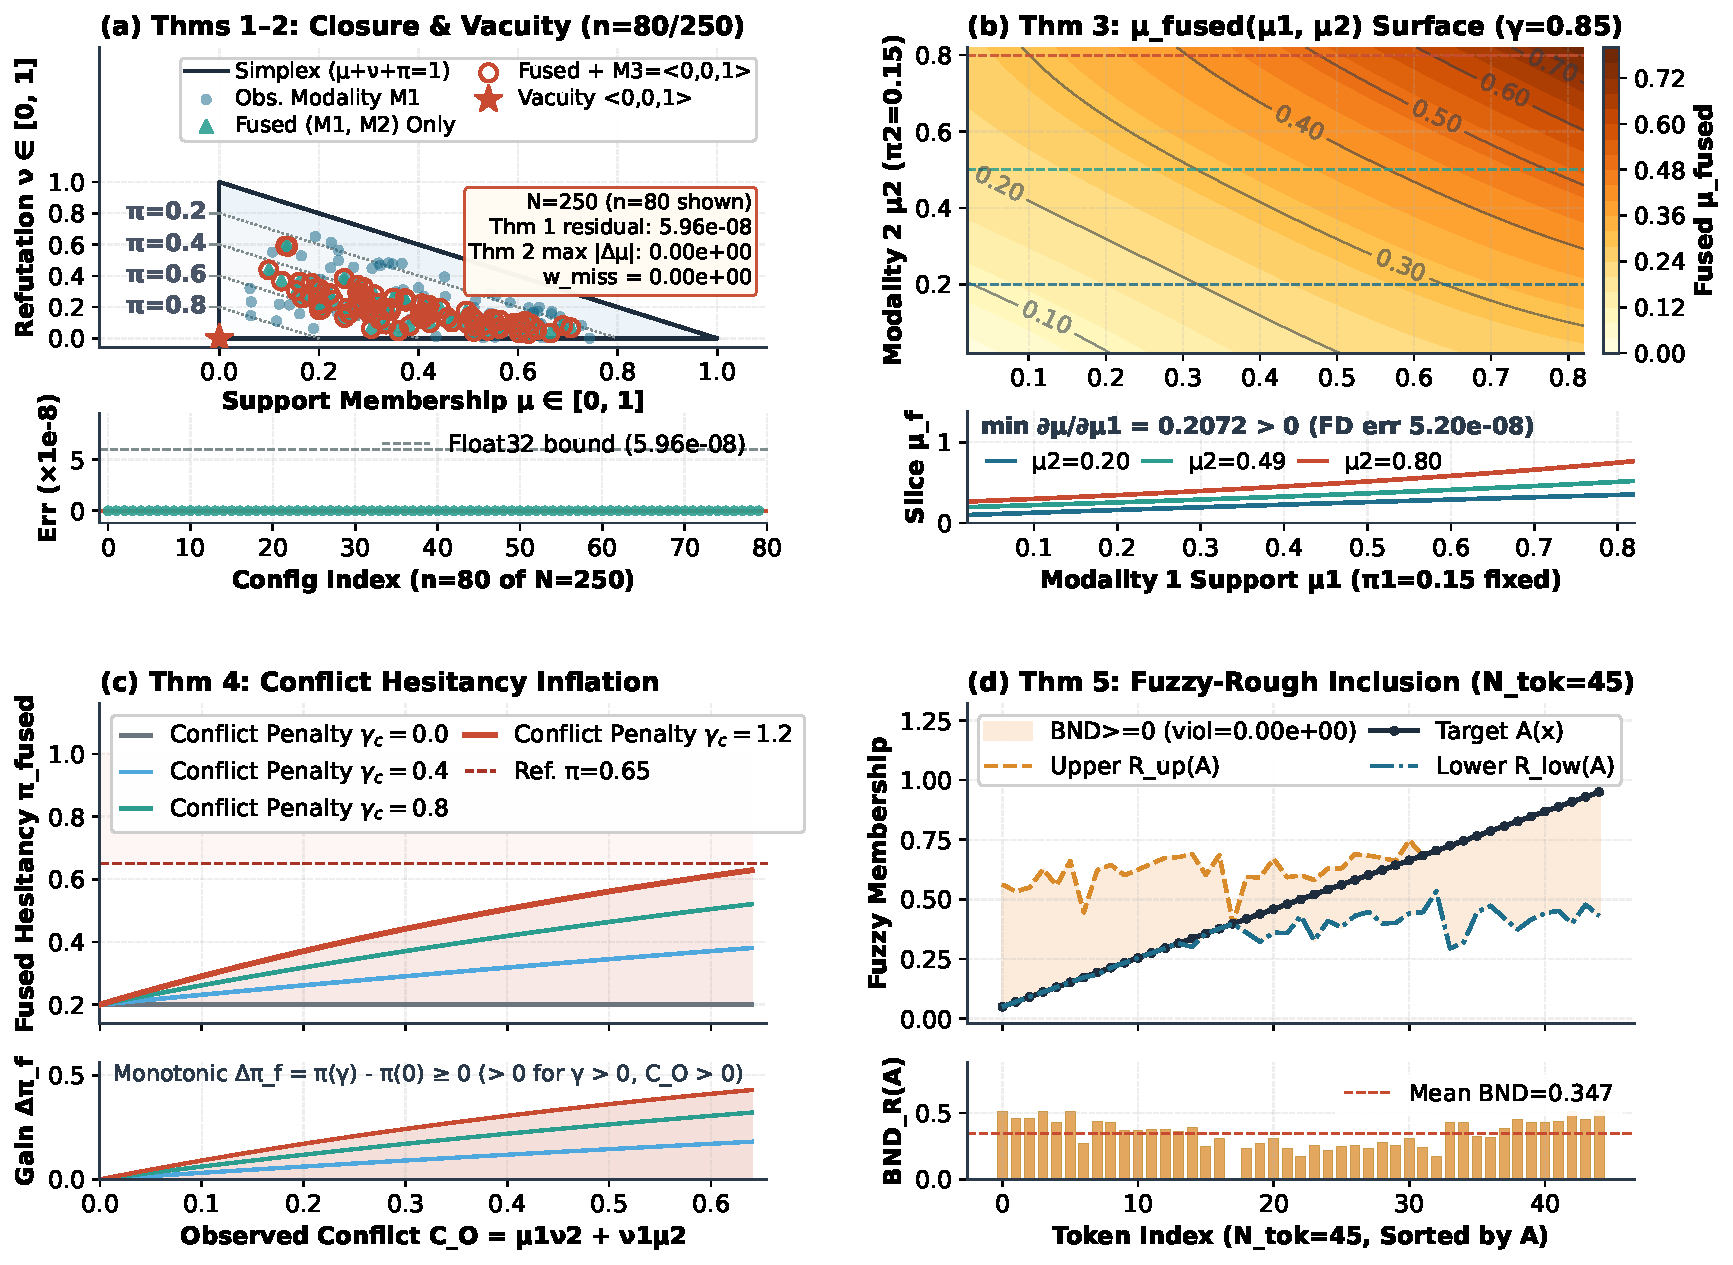
\includegraphics[width=\textwidth]{../figures/Fig1_Mathematical_Theorems_Verification.pdf}
    \caption{\textbf{Numerical verification of Theorems~\ref{thm:closure}--\ref{thm:rough}.}
    \textbf{(a)} Simplex closure ($\mu+\nu+\pi=1$, max float32 residual $5.96\times 10^{-8}$
    over $N=250$ \texttt{IntuitionisticFuzzyEncoder} inputs and $N=250$ directly sampled
    simplex tuples; $n=80$ subsampled directly sampled points plotted) and missing-modality
    vacuity invariance ($N=250$ four-modality tuples, $\gamma=0.85, \eta=0.9, p=1.2849$,
    deviation $0.00\times 10^0$). \textbf{(b)} Empirical surface $\mu_{\text{fused}}(\mu_1,
    \mu_2)$ over a $40\times 40$ grid at $r_1=r_2=0.85$ (frozen-discount partial derivative
    $\ge 0.2072>0$, analytic-vs-FD error $5.20\times 10^{-8}$). \textbf{(c)} Monotonic
    hesitancy inflation $\pi_{\text{fused}}(C_{\mathcal{O}})$ over 50 points spanning
    $C_{\mathcal{O}}\in[0,0.64]$ at fixed $r_m=0.80$. \textbf{(d)} Soft-{\L}ukasiewicz
    bounds $\underline{R}_\tau(A) \le A(x) \le \overline{R}_\tau(A)$ across $N_{\text{tok}}=45$
    tokens ($0.00\times 10^0$ inclusion violation).}
    \label{fig:theorems}
\end{figure*}
Figure~\ref{fig:theorems} summarizes the empirical verification of the five mathematical
properties formalized in Methods (Section~\ref{sec:method},
Theorems~\ref{thm:closure}--\ref{thm:rough}) under their respective experimental designs. For
Theorem~\ref{thm:closure}, we verified simplex closure $\mu + \nu + \pi = 1$ across both
$N=250$ random inputs mapped through \texttt{IntuitionisticFuzzyEncoder} and $N=250$
directly sampled Atanassov simplex IFN tuples fused with conflict penalty $\gamma=0.85$,
with a maximum float32 closure residual of $\max |\mu + \nu + \pi - 1| = 5.96 \times 10^{-8}$
while Figure~\ref{fig:theorems}(a) plots $n=80$ subsampled pairs from the directly sampled
simplex batch. For Theorem~\ref{thm:degeneration}, inserting a vacuous modality $\langle
0,0,1\rangle$ across all 5 modality positions of $N=250$ four-modality simplex tuples under
non-uniform fuzzy density parameters $\bm{\theta}=[-1.3, 0.27, 2.1, -0.4]$ and $\eta = 0.9$
($p = \exp(0.35\tanh(0.9)) = 1.2849$) yielded a maximum absolute deviation of
$0.00 \times 10^0$ and missing Choquet weight $w_{\text{miss}} = 0.00 \times 10^0$ in both
float32 and canonical-order float64, while Corollary~\ref{cor:e2e_vacuity} held end-to-end
across \texttt{UnifiedDeepFuzzyModel} with $0.00$ padding sensitivity.
Figure~\ref{fig:theorems}(b) displays the coupled surface $\mu_{\text{fused}}(\mu_1, \mu_2)$
over a $40 \times 40$ grid at $r_1=r_2=0.85$ and $\gamma=0.85$, where
Theorem~\ref{thm:monotonicity}'s frozen-discount partial derivative achieves minimum value
$0.2072 > 0$ with $5.20 \times 10^{-8}$ analytic-vs-FD error.
Figure~\ref{fig:theorems}(c)--(d) confirm Theorem~\ref{thm:conflict} across a 50-point sweep
over $C_{\mathcal{O}} \in [0, 0.64]$ at fixed $r_m=0.80$ for $\gamma \in \{0.0, 0.4, 0.8,
1.2\}$ and Theorem~\ref{thm:rough} across $N_{\text{tok}}=45$ tokens ($0.00 \times 10^0$
violation of $\underline{R}_\tau(A) \le A \le \overline{R}_\tau(A)$).

\subsection{Comparison with State-of-the-Art Fusion Methods and Equalized-Supervision Audit}

\begin{table*}[t]
\centering
\caption{\textbf{5-Fold Cross-Validation Performance and Supervision/Ablation Controls on ADNI
Cohort~1 ($N=1,137$ Full Cohort With Natural Missingness; Same-Visit Baseline Amyloid Reference
$n=924$; Complete 4-Modality Subset $N_{\text{comp}}=854$).} Top: comparison against fourteen
classical, evidential, recent 2023--2025 fusion, and tabular GBDT/foundation comparators under
identical folds (with $6/1,137$ [$0.53\%$] missing \texttt{ADAS13} entries imputed strictly
in-fold using training-fold medians). Bottom: supervision and joint-ablation controls equipping
\texttt{DempsterShafer\_EqLoss} and \texttt{GatedAttention\_EqLoss} with
$\text{BCE}+0.35\,\text{Brier}+0.75\,\text{AuxBCE}$ over distinct unimodal heads. Because
\texttt{EarlyConcatMLP} lacks unimodal heads (\texttt{modality\_probs[m]=prob}),
\texttt{EarlyConcat\_EqLoss}$^*$ receives shared fused-prediction weighting
$(1+0.75|\mathcal{O}_i|/M)\,\text{BCE}(p_{\text{fused}},y) +
0.35\,\text{Brier}(p_{\text{fused}},y)$ ($1.75\,\text{BCE}+0.35\,\text{Brier}$ at
$|\mathcal{O}_i|=4$), contrasted with \texttt{DeepFuzzyTorch\_ColdNoAux} (joint cold-start plus
no Brier/unimodal auxiliary BCE, $\lambda_{\text{aux}}=0$). Mathematical column winners in each
panel are in \textbf{bold}; two-sided paired bootstrap $p$-values and Benjamini--Hochberg
$q_{\text{BH}}$ (adjusted across all $m=20$ Cohort-1 baseline and ablation comparisons) compare
full-cohort ($N=1,137$) AUROC against \texttt{DeepFuzzyTorch}.}
\label{tab:adni_main}
\scriptsize
\setlength{\tabcolsep}{1.8pt}
\renewcommand{\arraystretch}{1.05}
\resizebox{\textwidth}{!}{%
\begin{tabular}{@{}>{\raggedright\arraybackslash}p{4.05cm}ccccccccccccc@{}}
\toprule
\textbf{Fusion / Tabular Method} & \shortstack{\textbf{Full
AUROC}\\\textbf{($N=1,137$,}\\\textbf{95\%
CI)}} & \shortstack{\textbf{Base}\\\textbf{Ref}\\\textbf{($n=924$)}} &
\shortstack{\textbf{Comp 4M}\\\textbf{($N_{\text{comp}}$}\\\textbf{=854)}} & \textbf{AUPRC} &
\textbf{Acc} & \textbf{F1} & \textbf{Brier} $\downarrow$ & \textbf{ECE} $\downarrow$ &
\textbf{AURC} $\downarrow$ & \shortstack{\textbf{15-Sub}\\\textbf{AUROC}\\\textbf{(Full/Elig)}}
& \shortstack{\textbf{Incomp}\\\textbf{MRR}} & \textbf{$p$-val} & \textbf{$q_{\text{BH}}$} \\
\midrule
EarlyConcat-MLP (\textit{TPAMI'19}) \cite{baltrusaitis2018multimodal} &
\shortstack{0.8212\\(0.7961--0.8434)} & 0.8304 & 0.8260 & 0.8693 & 0.7414 & 0.7443 & 0.1704 &
0.0431 &
0.1268 & 0.7690/0.7723 & 0.9318 & 0.350 & 0.769 \\
LateAvg-Ensemble (\textit{TPAMI'19}) \cite{baltrusaitis2018multimodal} &
\shortstack{0.8262\\(0.8010--0.8481)} & 0.8382 & 0.8346 & 0.8657 & 0.7502 & 0.7625 & 0.1724 &
0.0655 &
0.1543 & 0.7773/0.7811 & 0.9365 & 0.913 & 0.932 \\
DeepTSK-RuleNet (\textit{TFS'20}) \cite{wu2020optimize} & \shortstack{0.8086\\(0.7804--0.8334)}
& 0.8242 & 0.8181 & 0.8413 & 0.7573 & 0.7587 & 0.1781 & 0.0711 & 0.1462 & 0.7554/0.7591 &
0.9295 & 0.010
& 0.100 \\
Dempster--Shafer Fusion (\textit{IJAR'19}) \cite{denoeux2019decision} &
\shortstack{0.8115\\(0.7855--0.8357)} & 0.8242 & 0.8220 & 0.8523 & 0.7291 & 0.7403 & 0.1761 &
0.0371 & 0.1643 & 0.7668/0.7716 & \textbf{0.9409} & 0.032 & 0.213 \\
GatedAttention-Transformer (\textit{NCA'20}) \cite{vaswani2017attention,arevalo2017gated} &
\shortstack{0.8298\\(0.8040--0.8527)} & 0.8437 & 0.8403 & 0.8728 & 0.7546 & 0.7593 & 0.1676 &
0.0570 &
0.1214 & 0.7680/0.7717 & 0.9202 & 0.652 & 0.869 \\
EvidentialDL (TMC, \textit{TPAMI'23}) \cite{han2022trusted} &
\shortstack{0.8289\\(0.8036--0.8507)} & 0.8413 & 0.8378 & 0.8685 & 0.7537 & 0.7631 & 0.1676 &
0.0416 &
0.1456 & 0.7761/0.7800 & 0.9319 & 0.696 & 0.870 \\
RCML (adapted, \textit{AAAI'24}) \cite{xu2024reliable} & \shortstack{0.8229\\(0.7968--0.8456)}
& 0.8366 & 0.8340 & 0.8632 & 0.7493 & 0.7587 & 0.1752 & 0.0760 & 0.1333 & 0.7742/0.7781 &
0.9366 & 0.458
& 0.769 \\
QMF (Zhang et al., \textit{ICML'23}, adapt.) \cite{zhang2023provable} &
\shortstack{0.8313\\(0.8071--0.8540)} & 0.8449 & 0.8394 & 0.8749 & 0.7608 & 0.7643 &
0.1639 & 0.0483 & 0.1244 & 0.7759/0.7795 & 0.9286 & 0.472 & 0.769 \\
DrFuse (adapted, \textit{AAAI'24}) \cite{yao2024drfuse} &
\shortstack{0.8316\\(0.8062--0.8528)} & 0.8411 & 0.8389 & 0.8757 & 0.7493 &
0.7587 & 0.1660 & 0.0481 & 0.1265 & 0.7690/0.7730 & 0.9193 & 0.463 & 0.769 \\
DDEF (adapted, \textit{Inf.\ Fusion'24}) \cite{shao2024dual} &
\shortstack{0.8323\\(0.8069--0.8537)} & 0.8435 & 0.8414 & 0.8748 & 0.7520 & 0.7594 & 0.1674 &
0.0613 &
0.1319 & 0.7740/0.7776 & 0.9250 & 0.286 & 0.769 \\
FUML (adapted, \textit{ICML'25}) \cite{duan2025fuml} &
\shortstack{0.8363\\(0.8121--0.8584)} & 0.8477 & 0.8453 & 0.8759 & 0.7617 & 0.7690 & 0.1628 &
0.0279 &
0.1331 & \textbf{0.7790}/\textbf{0.7830} & 0.9266 & 0.052 & 0.260 \\
XGBoost (Native NaN) \cite{chen2016xgboost} &
\shortstack{0.8263\\(0.8009--0.8487)} & 0.8351 & 0.8333 & 0.8697 & 0.7493 & 0.7595 & 0.1733 &
0.0739 &
0.1254 & 0.7056/0.7125 & 0.8435 & 0.932 & 0.932 \\
CatBoost (NaN='Min') \cite{prokhorenkova2018catboost} &
\shortstack{0.8262\\(0.8009--0.8493)} & 0.8375 & 0.8370 & 0.8693 & 0.7546 & 0.7617 & 0.1705 &
0.0621 &
0.1239 & 0.7405/0.7438 & 0.8889 & 0.924 & 0.932 \\
TabPFN v2 (\textit{Nature'25}) \cite{hollmann2025tabpfn} &
\shortstack{\textbf{0.8443}\\\textbf{(0.8196--0.8664)}} & \textbf{0.8569} & \textbf{0.8541} &
\textbf{0.8844} & \textbf{0.7748} & \textbf{0.7782} & \textbf{0.1578} & \textbf{0.0269} &
\textbf{0.1101} & 0.7635/0.7668 & 0.8974 & 0.002 & 0.040 \\
\textbf{\texttt{DeepFuzzyTorch} (Ours)} & \shortstack{0.8270\\(0.8005--0.8486)} & 0.8387 &
0.8371 & 0.8680 & 0.7617 & 0.7686 & 0.1700 & 0.0651 & 0.1335 & 0.7764/0.7800 & 0.9344
& --- & --- \\
\midrule
\multicolumn{14}{@{}p{1.20\textwidth}@{}}{\textit{Supervision \& Joint-Ablation Controls
(\texttt{DempsterShafer}/\texttt{GatedAttention}: Unimodal $\text{AuxBCE}$;
\texttt{EarlyConcat}$^*$: Shared Fused AuxWeight; \texttt{ColdNoAux}: Joint Cold+NoBrier/Aux)}}
\\
EarlyConcat\_EqLoss$^*$ (Shared Fused AuxWeight) & \shortstack{0.8213\\(0.7957--0.8435)} & ---
& --- & 0.8694 & 0.7441 & 0.7476 & 0.1705 & 0.0383 & 0.1265 & 0.7686/--- & 0.9312 & 0.364 & ---
\\
DempsterShafer\_EqLoss & \shortstack{0.8101\\(0.7836--0.8341)} & --- & --- & 0.8502 & 0.7326 &
0.7437
& 0.1769 & \textbf{0.0316} & 0.1639 & 0.7674/--- & \textbf{0.9435} & 0.024 & --- \\
GatedAttention\_EqLoss & \shortstack{\textbf{0.8313}\\\textbf{(0.8055--0.8542)}} & --- & --- &
\textbf{0.8735} & \textbf{0.7661} & \textbf{0.7695} & \textbf{0.1663} & 0.0569 &
\textbf{0.1212} & 0.7714/--- & 0.9228 & 0.464 & --- \\
\texttt{DeepFuzzyTorch\_ColdNoAux} (Joint Cold, No Brier/Aux) &
\shortstack{0.8300\\(0.8046--0.8519)} & --- & --- & 0.8700 & 0.7493 & 0.7639 & 0.1694 & 0.0639
&
0.1468 & 0.7740/--- & 0.9278 & 0.384 & --- \\
\texttt{DeepFuzzyTorch} (Standard, Eq.~\eqref{eq:total_loss}) &
\shortstack{0.8270\\(0.8005--0.8486)} & --- & --- & 0.8680 & 0.7617 & 0.7686 & 0.1700 & 0.0651
&
0.1335 & \textbf{0.7764}/--- & 0.9344 & --- & --- \\
\bottomrule
\end{tabular}%
}
\end{table*}

Table~\ref{tab:adni_main} separates the three ADNI Cohort~1 evaluation populations: the full
natural-missingness cohort ($N=1,137$), the same-visit baseline amyloid reference ($n=924$),
and
the strictly complete four-modality subset ($N_{\text{comp}}=854$ participants observed across
all
four baseline modalities). Across the full cohort ($N=1,137$), \texttt{DeepFuzzyTorch} achieves
an
AUROC of $0.8270$ (95\% CI: $0.8005\text{--}0.8486$; accuracy $0.7617$, F1 $0.7686$), rising to
$0.8387$ on $n=924$ and $0.8371$ (95\% CI: $0.8091\text{--}0.8612$; AUPRC $0.8755$, accuracy
$0.7635$, F1 $0.7720$, Brier $0.1664$, ECE $0.0692$, AURC $0.1284$) on $N_{\text{comp}}=854$.
After Benjamini--Hochberg correction across all $m=20$ Cohort-1 comparisons,
\texttt{DeepFuzzyTorch} shows no statistically significant AUROC difference from the thirteen
neural, evidential, fuzzy, and gradient-boosted tree comparators ($q_{\text{BH}}\ge 0.100$ on
$N=1,137$; $q_{\text{BH}}\ge 0.180$ on $N_{\text{comp}}=854$). Several have slightly higher
point estimates, including \texttt{FUML (adapted)} ($0.8363/0.8453$,
$q_{\text{BH}}=0.260/0.368$) and \texttt{DDEF (adapted)} ($0.8323/0.8414$,
$q_{\text{BH}}=0.769/0.895$), without significant differences. It shows nominal unadjusted
$p<0.05$ versus \texttt{DeepTSK-RuleNet} ($0.8086$, raw $p=0.010$) and
\texttt{Dempster--Shafer} ($0.8115$, raw $p=0.032$), which does not remain significant after
BH multiplicity control ($q_{\text{BH}}=0.100$ and $q_{\text{BH}}=0.213$, respectively).
Pretrained \texttt{TabPFN~v2} alone attains a statistically significant AUROC advantage
($0.8443/0.8541$, $q_{\text{BH}}=0.040$), reflecting strong tabular prior capacity when
clinical scores and missingness indicators co-occur. Crucially, however,
single-table predictors (\texttt{XGBoost} MRR $0.8435$, \texttt{CatBoost} $0.8889$,
\texttt{TabPFN~v2} $0.8974$) suffer marked missing-modality drops and lack explicit
$C_{\mathcal{O}}$
conflict decomposition, whereas \texttt{DeepFuzzyTorch} maintains high incomplete-subset
retention ($\text{MRR}=0.9344$, 15-subset macro AUROC $0.7764 / 0.7800$ alongside
\texttt{FUML (adapted)} at $0.7790 / 0.7830$).

The bottom panel of Table~\ref{tab:adni_main} clarifies supervision and initialization effects:
jointly removing correlation warm-starting plus Brier and unimodal auxiliary BCE
(\texttt{DeepFuzzyTorch\_ColdNoAux}, $\lambda_{\text{aux}}=0$) reaches a full-cohort
($N=1,137$) AUROC of $0.8300$ (accuracy $0.7493$), whereas standard Eq.~\eqref{eq:total_loss}
improves accuracy ($0.7493 \to 0.7617$), selective risk AURC ($0.1468 \to 0.1335$), and
15-subset missingness robustness ($0.7740 \to 0.7764$). Conversely, equipping
\texttt{DempsterShafer\_EqLoss} ($0.8101$) and \texttt{GatedAttention\_EqLoss} ($0.8313$) with
Brier and unimodal auxiliary supervision, or applying matched shared-fused weighting
$(1+0.75|\mathcal{O}_i|/M)\,\text{BCE}+0.35\,\text{Brier}$ to \texttt{EarlyConcat\_EqLoss}$^*$
($0.8213$), leaves their 15-subset missing-modality AUROC gap relative to
\texttt{DeepFuzzyTorch}
intact ($0.7714$ vs.\ $0.7764$ on \texttt{GatedAttention\_EqLoss}).

\subsection{Ablation Study}

Supplementary Table~\ref{tab:ablation} dissects each operator's role. Removing exact vacuity
masking
($\langle 0,0,1\rangle \to$ zero imputation) slightly raises full-cohort ($N=1,137$) AUROC
($0.8286$,
$p=0.318$) because learned bias offsets exploit missingness indicators, but degrades 15-subset
macro AUROC from 0.7764 to 0.7690 and drops incomplete-subset Missing Robustness Retention
(MRR) from \textbf{0.9344} to 0.9230. Replacing non-additive Choquet capacities with uniform
$1/|\mathcal{O}|$ weighting worsens calibration ECE from 0.0651 to 0.0953, AURC from 0.1335 to
0.1383, and 20\%
conflict-referral AUROC from 0.8302 to 0.8218. Setting $\gamma=0$ degrades full-cohort
selective risk AURC ($0.1335 \to 0.1446$; note that at $\gamma=0$ under synthetic plasma swaps,
baseline hesitancy ranking alone yields 0.8355 at 20\%
referral, whereas $\gamma > 0$ is required to inflate $\pi_{\text{fused}}$ monotonically with
$C_{\mathcal{O}}$). Eliminating Fuzzy-Rough reduction ($D=320$ unreduced MRI ROIs) lowers full
AUROC from 0.8270 to 0.8221, accuracy from 0.7617 to 0.7388, and 15-subset AUROC from 0.7764 to
0.7677 while requiring $5.49\times$ more MRI branch parameters ($30,045$ vs.\ $5,477$).
Finally, removing \texttt{DeepConceptTSKHead} yields an observed AUROC of $0.8280$ versus
$0.8270$ ($p=0.190$; ECE $0.0461$ vs.\ $0.0651$), showing no statistically significant
difference on this cohort (without claiming formal equivalence or noninferiority), while
retaining white-box rule exportability in the full model.

\subsection{Combinatorial Missing-Modality Analysis}

\begin{figure*}[t]
    \centering
    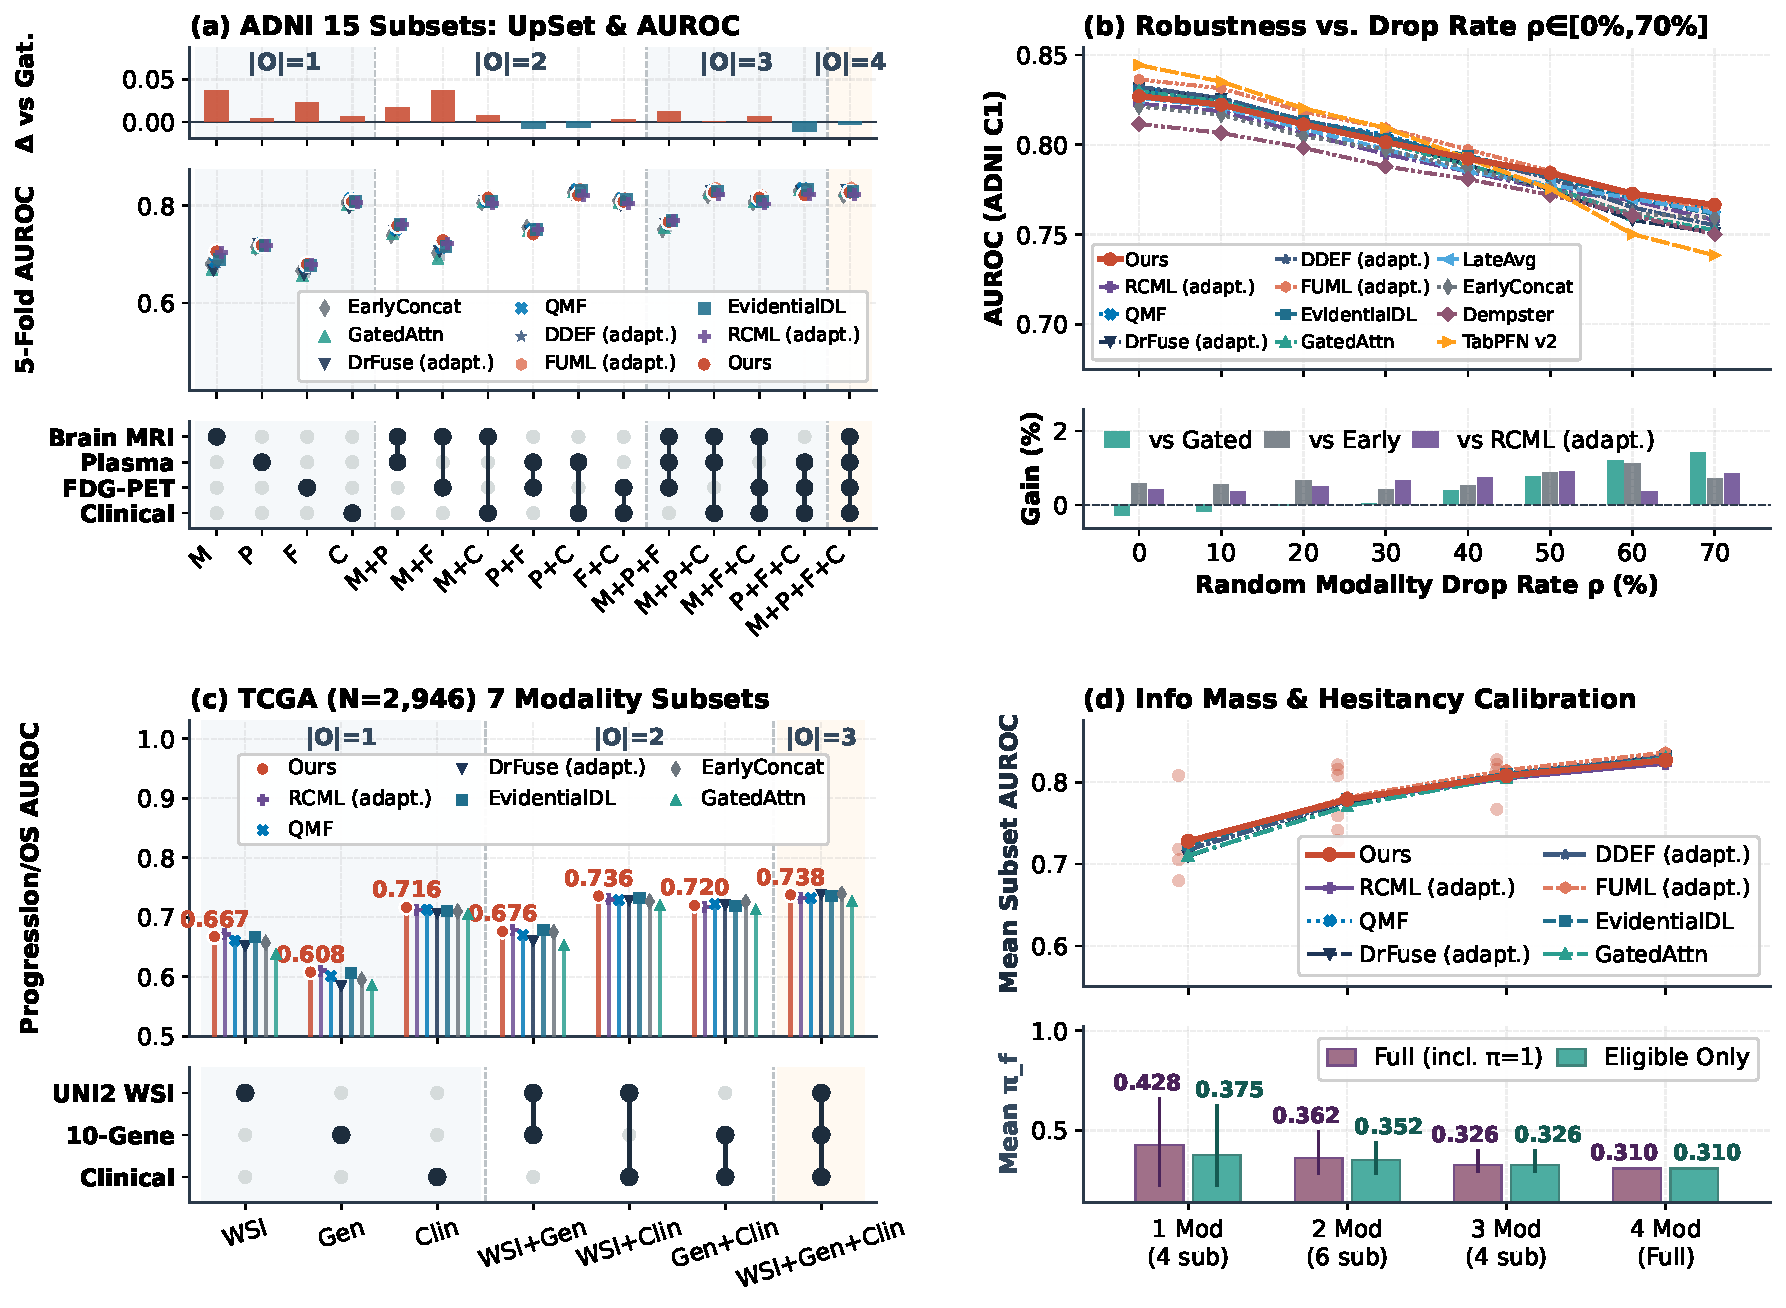
\includegraphics[width=\textwidth]{../figures/Fig2_Missing_Modality_Benchmark.pdf}
    \caption{\textbf{Combinatorial missing-modality evaluation.} \textbf{(a)} AUROC across all
    15 nonempty modality subsets on ADNI Cohort~1 ($N=1,137$). \textbf{(b)} Robustness under
    random modality drop rates $\rho \in [0, 0.7]$. \textbf{(c)} All 7 nonempty subsets on
    3-modality TCGA ($N=2,946$). \textbf{(d)} Monotonic contraction of mean hesitancy
    $\pi_{\text{fused}}$ ($0.428$ full-cohort / $0.375$ eligible at 1 modality $\to 0.310$ at 4
    modalities) alongside rising AUROC as observed modality count increases.}
    \label{fig:missing}
\end{figure*}

Supplementary Table~\ref{tab:missing_15} and Figure~\ref{fig:missing} evaluate all 15 nonempty
subsets on
ADNI Cohort~1 and all 7 subsets on TCGA Pan-Cancer ($N=2,946$). Across the nine joint neural,
evidential, and fuzzy architectures in Supplementary Table~\ref{tab:missing_15}, \texttt{FUML
(adapted)}
reaches $0.7790 / 0.7830$ macro AUROC (assisted by higher baseline 4-modality capacity), and
\texttt{DeepFuzzyTorch} places second at $0.7764 / 0.7800$ while surpassing
\texttt{EvidentialDL} ($0.7761$), \texttt{QMF (adapted)} ($0.7759$), \texttt{RCML (adapted)}
($0.7742$),
\texttt{DDEF (adapted)} ($0.7740$), \texttt{DrFuse (adapted)} ($0.7690$), \texttt{EarlyConcat}
($0.7690$), and \texttt{GatedAttention} ($0.7680$). Furthermore, \texttt{DeepFuzzyTorch}
attains
higher incomplete-subset retention ($\text{MRR} = 0.9344 / 0.9392$) than \texttt{FUML
(adapted)}
($0.9266$), \texttt{DDEF (adapted)} ($0.9250$), \texttt{QMF (adapted)} ($0.9286$),
\texttt{EvidentialDL}
($0.9319$), \texttt{GatedAttention} ($0.9202$), and \texttt{DrFuse (adapted)} ($0.9193$), as
well
as single-table predictors \texttt{TabPFN~v2} ($0.7635 / 0.7668$, $\text{MRR}=0.8974$),
\texttt{CatBoost} ($0.7405 / 0.7438$, $\text{MRR}=0.8889$), and \texttt{XGBoost} ($0.7056 /
0.7125$, $\text{MRR}=0.8435$). Notably, single-table GBDTs and \texttt{TabPFN~v2} degrade
steeply
on neuroimaging-only subsets such as \texttt{FDG} ($0.4777$, $0.5129$, and $0.5510$ vs.\
\texttt{DeepFuzzyTorch} $0.6797$) and \texttt{MRI} ($0.5515$, $0.6584$, and $0.6631$ vs.\
\texttt{DeepFuzzyTorch} \textbf{0.7054}). By contrast, \texttt{DeepFuzzyTorch}'s decoupled IFN
encoders and exact vacuity masking ($\langle 0,0,1\rangle$) lead joint models on \texttt{MRI}
(\textbf{0.7054 / 0.7071}), \texttt{FDG} eligible (\textbf{0.6907}), and \texttt{MRI+FDG}
(\textbf{0.7288}), while mean $\pi_{\text{fused}}$ contracts monotonically from $0.428$
full-cohort ($0.375$ eligible) at 1 modality to $0.310$ at 4 modalities
(Figure~\ref{fig:missing}(d)).

\begin{figure*}[t]
    \centering
    \includegraphics[width=\textwidth]{../figures/Fig3_%
Conflict_Injection_and_Selective_Referral.pdf}
    \caption{\textbf{Cross-modal conflict and selective referral.} \textbf{(a)} Hesitancy
    $\pi_{\text{fused}}$ and conflict $C_{\mathcal{O}}$ inflation under synthetic
    opposite-class biomarker swaps ($\gamma=0.8$, $n=262$ of $N_{\text{elig}}=872$).
    \textbf{(b)} Conflict detection AUROC across swap severity $\gamma$. \textbf{(c)}
    Full-cohort ($N=1,137$) selective referral curves ranked by $0.5\pi_{\text{fused}} + 0.5
    C_{\mathcal{O}}$. \textbf{(d)} Strictly nested outer-fold real-world biomarker discordance
    ($N=1,112$ deduplicated ADNI plasma participants, $1.51\times$, $p=1.75\times 10^{-17}$)
    and exploratory renal (CKD, $n=22$) stratification in ADNI Cohort~2.}
    \label{fig:conflict}
\end{figure*}

\subsection{Robustness to Cross-Modal Evidence Conflict}
Figure~\ref{fig:conflict} evaluates model behavior under synthetic intra-fold biomarker
conflict on ADNI Cohort~1, strictly nested real-world clinical biomarker discordance across
ADNI Cohorts~1 and~2 ($N=1,112$ deduplicated unique participants), and observational renal
confounding on ADNI Cohort~2 ($N=289$). In the synthetic stress test
(Figure~\ref{fig:conflict}(a)--(c)), $30\%$ of observed-plasma recipients ($n=262$ of
$N_{\text{elig}}=872$) are paired with opposite-class donors from the same validation fold via
\texttt{opposite\_swap} interpolation $x_{\text{corr}} = (1-\gamma)x_{\text{rec}} +
\gamma(2x_{\text{don}} - x_{\text{rec}})$. At $\gamma=0.8$, \texttt{DeepFuzzyTorch}'s average
observed-pair conflict $C_{\mathcal{O}}$ on $N_{\text{elig}}=872$ rises from $0.1317$ (clean
patients) to $0.1883$ (conflicted patients), hesitancy $\pi_{\text{fused}}$ inflates from
$0.3075$
to $0.3254$, and the composite triage score $0.5\,C_{\mathcal{O}} + 0.5\,\pi_{\text{fused}}$
discriminates corrupted from clean samples with $0.6542$ AUROC (Figure~\ref{fig:conflict}(b)).
Separating the two components reveals why: pure observed-pair conflict $C_{\mathcal{O}}$
achieves
\textbf{0.7000} anomaly AUROC---outperforming \texttt{QMF (adapted)} ($0.6667$),
\texttt{DrFuse (adapted)}
($0.6602$), \texttt{DDEF (adapted)} ($0.5888$ composite / $0.6892$ conflict-only), \texttt{FUML
(adapted)} ($0.5266$ / $0.6644$), \texttt{RCML (adapted)} ($0.6455$ / $0.6857$),
\texttt{EvidentialDL} ($0.5892$ / $0.6965$), and single-table predictors
($0.5557\text{--}0.5915$,
which lack explicit $C_{\mathcal{O}}$ decomposition)---whereas pure $\pi_{\text{fused}}$ yields
$0.5337$ because missing-modality vacuity dominates marginal hesitancy. Crucially, in
full-cohort ($N=1,137$) selective referral ranked by $0.5\pi_{\text{fused}} + 0.5
C_{\mathcal{O}}$ (Figure~\ref{fig:conflict}(c)), referring the top 20\%
highest-scoring cases restores retained-cohort diagnostic AUROC from $0.8062$ to $0.8302$ (and
to $0.8606$ at 40\% referral; $0.8307$ via pure $\pi_{\text{fused}}$ and $0.8136$ via pure
$C_{\mathcal{O}}$). At 20\% referral, \texttt{DeepFuzzyTorch} ($0.8302$) surpasses
\texttt{GatedAttention} ($0.8252$), \texttt{XGBoost} ($0.8256$), \texttt{QMF (adapted)}
($0.8212$),
\texttt{DrFuse (adapted)} ($0.8211$), \texttt{EvidentialDL} ($0.8178$), \texttt{EarlyConcat}
($0.8176$), \texttt{RCML (adapted)} ($0.8127$), \texttt{LateAvg} ($0.8076$),
\texttt{DempsterShafer} ($0.7868$), and \texttt{DeepTSK} ($0.7831$), while tracking
\texttt{CatBoost} ($0.8379$), \texttt{TabPFN~v2} ($0.8325$), \texttt{DDEF (adapted)}
($0.8308$), and \texttt{FUML (adapted)} ($0.8307$). Furthermore, on full ADNI Cohort~1 without
synthetic swaps ($N=1,137$), equal-coverage raw
out-of-fold composite ranking ($0.5\,\pi_{\text{fused}}+0.5\,C_{\mathcal{O}}$) yields
\texttt{DeepFuzzyTorch} accuracy of $0.7840$ (90\%), $0.8055$ (80\%), and $0.8229$ (70\%;
$\text{AURC}=0.1322$). This raw full-cohort ranking differs from the strictly nested outer-fold
training ECDF procedure in Supplementary Table~\ref{tab:matched_coverage} for $n=198$
discordant
participants,
and from the full-cohort pure-hesitancy $\text{AURC}=0.1335$ in
Tables~\ref{tab:adni_main}--\ref{tab:ablation}. At 80\% coverage, \texttt{TabPFN~v2} scores
$0.8209$ (AURC $0.1101$); \texttt{GatedAttention}, \texttt{DDEF (adapted)},
\texttt{FUML (adapted)}, \texttt{XGBoost}, and \texttt{CatBoost} score $0.8044$, $0.8011$,
$0.7989$, $0.7945$, and $0.7923$, respectively.

To audit real-world cross-modal contradiction without synthetic perturbation or quantile
leakage, we define biomarker discordance strictly using training-fold medians across ADNI
Cohort~1 ($n=872$ observed plasma pTau181) and Cohort~2 ($N=289$ plasma pTau217/GFAP). A
patient is discordant if plasma pTau meets or exceeds the training-fold median despite both
preserved hippocampal volume ($>$ training-fold median \texttt{Hippocampus\_\allowbreak
ICV\_\allowbreak ratio}) and unimpaired baseline cognition ($\texttt{DX\_bl}=\texttt{CN}$,
$\text{CDRSB}<0.5$), or if plasma pTau falls below median despite both hippocampal atrophy and
cognitive impairment. In Cohort~1 ($n=872$), $n_{\text{disc}}=159$ discordant patients exhibit
$1.49\times$ higher $C_{\mathcal{O}}$ than $n_{\text{conc}}=713$ concordant patients ($0.1781$
vs.\ $0.1198$, two-sided Mann--Whitney $p = 4.94 \times 10^{-18}$); in Cohort~2 ($N=289$),
$n_{\text{disc}}=47$ discordant patients exhibit $1.58\times$ higher $C_{\mathcal{O}}$ than
$n_{\text{conc}}=242$ concordant patients ($0.2167$ vs.\ $0.1372$, $p = 1.39 \times 10^{-3}$).
Across the deduplicated union of unique ADNI plasma participants ($N=1,112$ unique
\texttt{RID}s; Figure~\ref{fig:conflict}(d)), $n_{\text{disc}}=198$ discordant patients exhibit
$1.51\times$ higher observed-pair conflict $C_{\mathcal{O}}$ than $n_{\text{conc}}=914$
concordant patients ($0.1871$ vs.\ $0.1242$, Mann--Whitney $p = 1.75 \times 10^{-17}$;
composite score $0.2619$ vs.\ $0.2055$, $p = 1.58 \times 10^{-15}$). Under raw outer-training
80th-percentile referral cutoffs (Supplementary Table~\ref{tab:matched_coverage}, column~2),
GBDTs suffer
severe threshold shrinkage---retaining only $32.3\%$ ($64/198$) for \texttt{CatBoost}
($0.9062$)
and $50.0\%$ ($99/198$) for \texttt{XGBoost} ($0.8384$)---which inflates uncalibrated triage
accuracy relative to \texttt{DeepFuzzyTorch} ($0.7764$, $125/161$ at $81.3\%$ retained).
Evaluating exact accuracy at equalized coverages via strictly nested outer-fold ECDF
calibration
(Supplementary Table~\ref{tab:matched_coverage} and Figure~\ref{fig:conflict}(d) right)
eliminates this
shrinkage artifact: at $81.3\%$ ($161/198$) and $80\%$ ($158/198$) retained coverage,
\texttt{DeepFuzzyTorch} composite achieves $0.7764 / 0.7785$ ($\text{AURC}=0.1671$) and pure
$C_{\mathcal{O}}$ ECDF reaches $0.7826 / 0.7911$, outperforming \texttt{CatBoost} ($0.7516 /
0.7595$), \texttt{XGBoost} ($0.7391 / 0.7468$), \texttt{DDEF (adapted)} ($0.7516 / 0.7595$),
\texttt{RCML (adapted)} ($0.7453 / 0.7468$), and \texttt{FUML (adapted)} ($0.7391 / 0.7342$),
while trailing
\texttt{TabPFN~v2} ($0.8012 / 0.8101$, $\text{AURC}=0.1248$, unadjusted paired bootstrap
$p=0.026$,
$q_{\text{BH}}=0.286$) and matching
\texttt{QMF (adapted)} ($0.7826 / 0.7848$) and \texttt{DrFuse (adapted)} ($0.7888 / 0.7911$).
Across all 11
comparator AURC tests, $q_{\text{BH}}\ge0.286$; none is significant after BH correction.

On ADNI Cohort~2 ($N=289$, Supplementary Table~\ref{tab:external_ckd}), where high-specificity
plasma pTau217
already provides strong unimodal signal (\texttt{UnimodalPlasma\_pTau217} AUROC $0.8739$),
\texttt{TabPFN~v2} ($0.8830$ on $N=289$; $0.8859$ on $\le 90$-day window $n=211$; $0.9037$ on
strict concurrent $n=176$), \texttt{RCML (adapted)} ($0.8782 / \textbf{0.8868} / 0.9010$),
\texttt{EvidentialDL} ($0.8762 / 0.8857 / \textbf{0.9045}$), \texttt{XGBoost} ($0.8749 / 0.8829
/
0.8983$), \texttt{CatBoost} ($0.8741 / 0.8830 / 0.8917$), \texttt{DeepFuzzyTorch} ($0.8740$
[95\% CI: $0.8331\text{--}0.9106$] / $0.8844$ / $0.8969$), \texttt{FUML (adapted)} ($0.8608 /
0.8697 / 0.8887$), and \texttt{DDEF (adapted)} ($0.8595 / 0.8640 / 0.8958$) show no
statistically
significant pairwise AUROC differences ($q_{\text{BH}} \ge 0.602$ across all twelve
comparators).
As an exploratory physiological proof-of-concept within the small measured chronic kidney
disease subgroup (low baseline eGFR $<60\text{ mL/min/1.73m}^2$, single baseline
measurement; $n=22$ total: $n=6$ exploratory A$\beta^-$ CKD and $n=16$ A$\beta^+$),
A$\beta^-$ CKD subjects ($n=6$) display elevated mean plasma pTau217 ($0.2618$ vs.\
$0.1546\text{ pg/mL}$) and GFAP ($205.7$ vs.\ $164.1\text{ pg/mL}$) relative to A$\beta^-$
normal-renal subjects ($n=22$), accompanied by $3.58\times$ higher directional
plasma-versus-non-plasma conflict $\mu_{\text{Plasma}}\cdot
\frac{1}{3}(\nu_{\text{MRI}}+\nu_{\text{FDG}}+\nu_{\text{Clin}})$ ($0.1932$ vs.\ $0.0539$,
two-sided Mann--Whitney $p = 0.0448$). Under symmetric in-fold 80th-percentile composite triage
on $n=22$, retained accuracy rises from $0.7727$ ($17/22$) to $0.8421$ ($16/19$, exact 95\%
CI: 0.6042--0.9662; hesitancy-only $0.8000$ [$16/20$]) for \texttt{DeepFuzzyTorch} and
\texttt{EvidentialDL}. This compares with $0.9333$ ($14/15$) for \texttt{DrFuse (adapted)},
$0.8750$ ($14/16$) for \texttt{QMF (adapted)}, $0.8500$ ($17/20$) for \texttt{EarlyConcat},
$0.8333$
($15/18$) for \texttt{RCML (adapted)} and \texttt{GatedAttention}, and $0.7727 \to 0.8000$
($16/20$) for \texttt{PlasmaOnly}; given the wide binomial CIs at $n=22$, this renal subgroup
is strictly hypothesis-generating.

\begin{figure*}[t]
    \centering
    \includegraphics[width=\textwidth]{../figures/Fig4_%
Fuzzy_Rough_Reduct_and_MultiOmics_FM.pdf}
    \caption{\textbf{Fuzzy-rough feature selection and multi-source fusion.} \textbf{(a)}
    Pointwise T-norm positive dependency $\gamma_{\mathcal{B}}(D)$, permutation null
    $\gamma^{\text{null}}$, boundary $\operatorname{BND}_{\mathcal{B}}(D)$, and MRI OOF AUROC
    (peaking at $k=12$) versus subset size $k$, annotating the fixed budget $K^*=24$ and the
    inner-split composite objective peak ($\text{AUROC}_{\text{val}} +
    0.05\Delta\gamma_{\mathcal{B}_k} - 0.0008k$ at $k=20$). \textbf{(b)} Top-ranked FreeSurfer
    biomarkers by univariate dependency. \textbf{(c)} Per-cohort AUROC across 7 TCGA cancer
    types. \textbf{(d)} Six-foundation-model pathology consensus on Camelyon17 and the NCT-CRC
    binary tumor-or-stroma endpoint (\texttt{is\_tumor\_or\_stroma}) derived from the 9-class
    NCT-CRC-HE-100K / CRC-VAL-HE-7K dataset. Corruption applies a $-2\times$ sign-and-scale
    inversion to standardized PCA-64
    features on the held-out \texttt{plip} expert stream.}
    \label{fig:rough_tcga}
\end{figure*}

\begin{figure*}[t]
    \centering
    \includegraphics[width=\textwidth]{../figures/Fig6_%
HighDim_TCGA_Transcriptomic_Reduct_and_Reactome.pdf}
    \caption{\textbf{High-dimensional transcriptomic reduction on TCGA ($D_{\text{RNA}}=1,000$
    label-free transductive MAD genes, $N=2,946$).} \textbf{(a)} Pointwise T-norm fuzzy-rough
    dependency trajectory versus permutation null across $k=1\dots 30$, showing the fixed
    budget $K^*=20$, the inner-split composite objective peak ($\text{AUROC}_{\text{val}} +
    0.08\widetilde{\Delta\gamma}_{\mathcal{B}_k} - 0.0006k$ at $k=12$, with normalized excess
    $\widetilde{\Delta\gamma}_{\mathcal{B}_k} =
    \Delta\gamma_{\mathcal{B}_k}/(1-\gamma^{\text{null}}_{\mathcal{B}_k})$), and the RNA-only
    OOF AUROC curve (peaking at $k=28$). \textbf{(b)} Cross-fold consensus top-20 genes and
    fold-selection frequencies. \textbf{(c)} Custom-background Reactome pathway
    over-representation ($N_{\text{bg}}=1,000$, $k\ge 2$ unique genes: $8$ pathways at
    $q_{\text{BH}}<0.05$ across all $m=676$ predeclared $K_{\text{bg}}\ge 2$ background
    pathways). \textbf{(d)} Four-modality fusion comparing \texttt{FuzzyRough-20},
    matched-architecture \texttt{All-1000}, classical feature selectors, and adapted/recent
    baselines.}
    \label{fig:tcga_highdim}\label{fig:tcga_rnaseq}
\end{figure*}

\begin{table*}[t]
\centering
\caption{\textbf{TCGA Pan-Cancer Multi-Omics + Clinical Staging + Histopathology WSI Benchmark
($N=2,946$ Unique Patients Across 7 Cohorts) and 6-Foundation-Model Pathology Consensus
($N=4,849$ Patches/Tiles).} Top: 5-fold pan-cancer composite progression/mortality AUROC,
descriptive OS C-index, 7-subset missing-modality macro AUROC, and per-cohort AUROCs on
3-modality TCGA, followed by 4-modality (+ label-free transductive 1,000-gene MAD RNA-Seq)
baselines and Classical vs.\ Fuzzy-Rough feature selectors ($K^*=20$, reporting cross-fold
Jaccard stability and full-cohort RNA-only AUROC [$N=2,946$] in text). Bottom: 6-FM patch/tile
AUROC comparing source-CV \texttt{BestSingleFM} (\texttt{uni2\_h}), \texttt{MeanPool},
\texttt{MedianPool}, \texttt{Logit-Tent (adapted)} (\textit{ICLR'21}), source-OOF Adam-fitted
\texttt{HesitantFuzzy}, and \texttt{HesitantFuzzy + PFS TTA}. NCT-CRC evaluates the binary
\texttt{is\_tumor\_or\_stroma} endpoint derived from the 9-class NCT-CRC-HE-100K /
CRC-VAL-HE-7K dataset. The corrupted
scenario applies $-2\times$ sign-and-scale inversion to standardized PCA-64 features on the
held-out \texttt{plip} expert stream. Boldface marks mathematical column/row winners.}
\label{tab:tcga_fm}
\scriptsize
\renewcommand{\arraystretch}{0.84}
\setlength{\tabcolsep}{1.6pt}
\resizebox{\textwidth}{!}{%
\begin{tabular}{@{}>{\raggedright\arraybackslash}p{5.55cm}cccccccccc@{}}
\toprule
\textbf{Method} & \shortstack{\textbf{Pan-Cancer}\\\textbf{AUROC (95\%
CI)}} & \shortstack{\textbf{OS}\\\textbf{C-Idx}} & \textbf{7-Sub} &
\textbf{BRCA} & \textbf{COAD} & \textbf{KIRC} & \textbf{KIRP} & \textbf{LUAD} & \textbf{LUSC} &
\textbf{UCEC} \\
\midrule
EarlyConcat-MLP (\textit{TPAMI'19}, 3-Mod) \cite{baltrusaitis2018multimodal} &
\textbf{0.7394 (0.7195--0.7558)} & 0.7321 & 0.6898 & \textbf{0.7110} & 0.7036 & 0.8053 &
0.7094 & 0.6523 & 0.6528 & 0.6580 \\
GatedAttention-Transformer (\textit{NCA'20}, 3-Mod)
\cite{vaswani2017attention,arevalo2017gated} & 0.7268 (0.7059--0.7462) & 0.7164 & 0.6775 &
0.6974 & 0.6798 & 0.8097 & 0.6639 & 0.6277 & 0.6480 & 0.6507 \\
EvidentialDL (TMC, \textit{TPAMI'23}, 3-Mod) \cite{han2022trusted} &
0.7363 (0.7177--0.7542) & 0.7375 & 0.6928 & 0.6721 & 0.7200 & 0.8071 & 0.6983 & 0.6440 &
\textbf{0.6553} & 0.6673 \\
RCML (adapted, \textit{AAAI'24}, 3-Mod) \cite{xu2024reliable} & 0.7322 (0.7129--0.7504) &
0.7350 & 0.6931 & 0.6688 & 0.7266 & 0.7998 & 0.6955 & 0.6418 & 0.6525 & 0.6325 \\
QMF (\textit{ICML'23}, adapt., 3-Mod) \cite{zhang2023provable} & 0.7321 (0.7116--0.7500) &
0.7276 &
0.6898 & 0.6680 & 0.7147 & 0.8000 & 0.7013 & 0.6361 & 0.6534 & 0.6517 \\
DrFuse (adapted, \textit{AAAI'24}, 3-Mod) \cite{yao2024drfuse} & 0.7376 (0.7177--0.7546) &
0.7227 & 0.6838 & 0.7043 & 0.7020 & 0.8204 & 0.6770 & 0.6410 & 0.6435 & \textbf{0.6729} \\
\textbf{\texttt{DeepFuzzyTorch} (Ours, 3-Mod)} & 0.7377 (0.7183--0.7561) & \textbf{0.7492} &
\textbf{0.6944} & 0.6624 & \textbf{0.7270} & \textbf{0.8227} & \textbf{0.7154} &
\textbf{0.6594} & 0.6432 & 0.6170 \\
\midrule
\texttt{DeepFuzzyTorch} (4-Mod, Matched \texttt{All-1000}) & 0.6925 (0.6725--0.7114) & 0.6933
& --- & --- & --- & --- & --- & --- & --- & --- \\
EarlyConcat-MLP (4-Mod, \texttt{All-1000}) \cite{baltrusaitis2018multimodal} &
0.6932 (0.6721--0.7123) & 0.6945 & --- & --- & --- & --- & --- & --- & --- & --- \\
GatedAttention (4-Mod, $K^*=20$) \cite{arevalo2017gated} & 0.7218 (0.7018--0.7388) & 0.7144 &
--- & --- & --- & --- & --- & --- & --- & --- \\
EarlyConcat-MLP (4-Mod, $K^*=20$) \cite{baltrusaitis2018multimodal} & 0.7320 (0.7116--0.7492) &
0.7365 & --- & --- & --- & --- & --- & --- & --- & --- \\
QMF (\textit{ICML'23}, adapt., 4-Mod, $K^*=20$) \cite{zhang2023provable} & 0.7338
(0.7145--0.7511) &
0.7330 & --- & --- & --- & --- & --- & --- & --- & --- \\
DrFuse (adapted, \textit{AAAI'24}, 4-Mod, $K^*=20$) \cite{yao2024drfuse} &
0.7340 (0.7152--0.7522) & 0.7284 & --- & --- & --- & --- & --- & --- & --- & --- \\
RCML (adapted, \textit{AAAI'24}, 4-Mod, $K^*=20$) \cite{xu2024reliable} &
0.7350 (0.7152--0.7524) & 0.7384 & --- & --- & --- & --- & --- & --- & --- & --- \\
DempsterShafer (\textit{IJAR'19}, 4-Mod, $K^*=20$) \cite{denoeux2019decision} &
0.7373 (0.7181--0.7547) & 0.7441 & --- & --- & --- & --- & --- & --- & --- & --- \\
EvidentialDL (\textit{TPAMI'23}, 4-Mod, $K^*=20$) \cite{han2022trusted} &
0.7377 (0.7184--0.7551) & 0.7413 & --- & --- & --- & --- & --- & --- & --- & --- \\
\texttt{DeepFuzzyTorch} + \texttt{mRMR-20} \cite{peng2005feature} (Sparse 20G, Jacc.\
\textbf{0.4696}) & 0.7378 (0.7187--0.7561) & 0.7528 & --- & --- & --- & --- & --- & --- &
--- & --- \\
\texttt{DeepFuzzyTorch} + \texttt{Lasso-20} ($L_1$-LogReg, Sparse 20G, Jacc.\ 0.1985) &
0.7398 (0.7206--0.7573) & 0.7508 & --- & --- & --- & --- & --- & --- & --- & --- \\
\textbf{\texttt{DeepFuzzyTorch} + \texttt{FuzzyRough-20} (Ours, Sparse 20G, Jacc.\ 0.3816)} &
0.7403 (0.7208--0.7579) & 0.7514 & --- & --- & --- & --- & --- & --- & --- & --- \\
\texttt{DeepFuzzyTorch} + \texttt{MI-20} (Mutual Info, Sparse 20G, Jacc.\ 0.1058) &
0.7417 (0.7227--0.7588) & 0.7520 & --- & --- & --- & --- & --- & --- & --- & --- \\
\texttt{DeepFuzzyTorch} + \texttt{PCA-20} (Dense 1,000-Gene Linear Proj., Non-Sparse) &
\textbf{0.7450 (0.7254--0.7625)} & \textbf{0.7569} & --- & --- & --- & --- & --- & --- & ---
& --- \\
\bottomrule
\end{tabular}%
}

\vspace{0.15em}

\setlength{\tabcolsep}{2.0pt}
\resizebox{\textwidth}{!}{%
\begin{tabular}{@{}>{\raggedright\arraybackslash}p{4.55cm}cccccc@{}}
\toprule
\textbf{6-Foundation-Model Pathology Benchmark Scenario} &
\shortstack{\textbf{BestSingleFM}\\\textbf{(Source \texttt{uni2\_h})}} &
\shortstack{\textbf{MeanPool}\\\textbf{(6 FMs)}} & \shortstack{\textbf{MedianPool}\\\textbf{(6
FMs)}} & \shortstack{\textbf{Logit-Tent}\\\textbf{(adapt.) \cite{wang2021tent}}} &
\shortstack{\textbf{HesitantFuzzy}\\\textbf{(Adam Source OOF)}} &
\shortstack{\textbf{HesitantFuzzy +}\\\textbf{PFS TTA (Ours)}} \\
\midrule
Camelyon17 ($N=2,500$ Patches: Source $n=1,500 \to$ OOD $n=1,000$, Clean) & \textbf{0.9942} &
0.9915 & 0.9909 & 0.9914 & 0.9919 & 0.9919 (0.9878--0.9956) \\
Camelyon17 ($n=1,000$ OOD Patches, 1 Corrupted Foundation Model) & \textbf{0.9942} & 0.9894 &
0.9912 & 0.9893 & 0.9922 & 0.9925 (0.9878--0.9962)$^\dagger$ \\
NCT-CRC Binary (\texttt{Discovery} $n=999 \to$ External \texttt{VAL\_7K} $n=1,350$ Tiles,
Clean) &
0.9760 & \textbf{0.9825} & 0.9818 & 0.9823 & 0.9814 & 0.9815 (0.9753--0.9871) \\
NCT-CRC Binary ($n=1,350$ External Tiles, 1 Corrupted Foundation Model) & 0.9760 & 0.9567 &
\textbf{0.9812} & 0.9561 & 0.9781 & 0.9804 (0.9739--0.9865) \\
\bottomrule
\multicolumn{7}{@{}p{1.05\textwidth}@{}}{\scriptsize $^\dagger$Highest AUROC among all 6-FM
multi-model ensemble/TTA methods on corrupted Camelyon17 ($q_{\text{BH}}=0.010$ vs.\
\texttt{MeanPool} and \texttt{Logit-Tent (adapted)}); uncorrupted \texttt{uni2\_h} serves as
single-FM reference. NCT-CRC Binary is the \texttt{is\_tumor\_or\_stroma} endpoint derived
from the 9-class NCT-CRC-HE-100K / CRC-VAL-HE-7K dataset. Corruption is a $-2\times$
sign-and-scale inversion of standardized PCA-64 features on the held-out \texttt{plip}
expert stream.}
\end{tabular}%
}
\end{table*}

\subsection{Fuzzy-Rough Reduction and Pan-Cancer Fusion}
Figure~\ref{fig:rough_tcga}(a)--(b) illustrate the 5-fold strictly in-fold pointwise T-norm
Fuzzy-Rough attribute selection trajectory on the 320 FreeSurfer MRI features of ADNI Cohort~1.
As subset size $k$ grows from 1 to 30, mean positive dependency $\gamma_{\mathcal{B}}(D)$
increases monotonically from 0.2246 to 0.6368 (above the label-permutation null
$\gamma^{\text{null}}$ from 0.2134 to 0.6293, with positive excess dependency $\Delta\gamma =
0.0112$ at $k=1$, peaking at $0.0148$ at $k=3$, and $0.0083$ at $k=24$), while boundary
uncertainty $\operatorname{BND}_{\mathcal{B}}(D)$ contracts monotonically from 0.7754 to 0.3632
(Theorem~\ref{thm:rough}, Part~II). At the prespecified fixed budget $K^*=24$ ($92.50\%$
feature compression and $81.77\%$ MRI branch parameter reduction), out-of-fold MRI-only AUROC
reaches 0.7010 (0.7084 at $k=30$) with cross-fold pairwise Jaccard stability $0.4330 \pm
0.1206$. Top univariate FreeSurfer biomarkers align with Braak neurofibrillary and vascular
white-matter pathology: white-matter hypointensities (\texttt{ST128SV}, $\gamma=0.2392$),
entorhinal cortex/ICV ratio ($\gamma=0.2318$), non-WM hypointensities (\texttt{ST68SV},
$\gamma=0.2284$), right caudate (\texttt{ST75SV}, $\gamma=0.2261$), left entorhinal volume
(\texttt{ST24CV}, $\gamma=0.2261$), bilateral middle/inferior temporal and entorhinal cortices
(\texttt{ST40TA}, \texttt{Middle\_Temporal\_ICV\_ratio}, \texttt{ST99TA}, \texttt{ST83TA},
\texttt{ST91TA}; $\gamma=0.2247\text{--}0.2255$), and bilateral hippocampus and amygdala
(\texttt{ST88SV}, \texttt{ST71SV}, \texttt{ST29SV}; $\gamma=0.2243\text{--}0.2247$).

On the 3-modality TCGA Pan-Cancer benchmark ($N=2,946$ unique patients, Table~\ref{tab:tcga_fm}
top and Figure~\ref{fig:rough_tcga}(c)), complete-modality discriminative performance is
tightly clustered across architectures ($q_{\text{BH}} \ge 0.181$): \texttt{EarlyConcat}
attains 0.7394, \texttt{DeepFuzzyTorch} attains 0.7377 (95\%
CI: 0.7183--0.7561), \texttt{DrFuse (adapted)} attains 0.7376, and \texttt{EvidentialDL}
attains 0.7363, while \texttt{DeepFuzzyTorch} achieves the highest descriptive OS C-index
(\textbf{0.7492}), highest 7-subset missing-modality macro AUROC (\textbf{0.6944}), and top
cohort AUROCs on COAD (\textbf{0.7270}), KIRC (\textbf{0.8227}), KIRP (\textbf{0.7154}), and
LUAD (\textbf{0.6594}).

To evaluate high-dimensional transcriptomic reduction on an unsupervised, label-free
transductive candidate pool without curated cancer-gene lists (Figure~\ref{fig:tcga_highdim}),
we apply \texttt{FuzzyRough\allowbreak Feature\allowbreak Reducer} with supervised in-fold
selection inside each training fold to the top $D_{\text{RNA}}=1,000$ MAD-filtered PanCancer
Atlas protein-coding genes ($n=2,929$ observed RNA-Seq; an in-fold top-$1,000$ MAD re-screening
inside the pooled transductive unsupervised $5,000$-gene MAD cache [$5,000 \to 1,000 \to 20$]
yields $0.9685$ candidate-pool Jaccard overlap and $0.7389$ 4-modality AUROC). Across $k=1 \to
20 \to 30$ (Figure~\ref{fig:tcga_highdim}(a)), $\gamma_{\mathcal{B}}(D)$ rises monotonically
($0.2120 \to 0.5958 \to 0.6148$) above $\gamma^{\text{null}}$ ($0.2076 \to 0.5863 \to 0.6059$),
$\operatorname{BND}_{\mathcal{B}}(D)$ contracts ($0.7880 \to 0.4042 \to 0.3852$), and
full-cohort ($N=2,946$) RNA-only OOF AUROC increases from $0.5905$ to $0.6458$ at fixed budget
$K^*=20$ ($0.6464$ on $n=2,929$ observed RNA-Seq; $98.0\%$ compression and $94.05\%$ RNA branch
parameter reduction from 86,485 to 5,145). Cross-fold consensus genes
(Figure~\ref{fig:tcga_highdim}(b)) are led by \texttt{IGF2BP3}, \texttt{SFTPA2},
\texttt{BARX1}, \texttt{HIF3A}, and \texttt{NTS} (5/5 folds), followed by \texttt{FGA},
\texttt{IL6}, \texttt{SFTPD}, \texttt{GPR87}, \texttt{AADAC}, and \texttt{PHACTR3} (4/5 folds).
Custom-background Reactome over-representation analysis against the exact 1,000-gene background
($N_{\text{bg}}=1,000$, 575 annotated, requiring $k \ge 2$ unique foreground genes;
Figure~\ref{fig:tcga_highdim}(c)) \cite{milacic2024reactome} identifies strictly $8$ pathways
passing $q_{\text{BH}}<0.05$ across all $m=676$ predeclared testable background pathways with
$K_{\text{bg}}\ge 2$. These $8$ FDR-significant pathways comprise \textit{Regulation of TLR by
endogenous ligand} (\texttt{R-HSA-5686938}, $k=3/6$ [\texttt{FGA}, \texttt{SFTPA2},
\texttt{SFTPD}], $25.0\times$ enrichment, $p=1.32\times 10^{-4}$, $q_{\text{BH}}=0.0308$), four
\textit{TLR4/TLR2} surfactant-ligand cascades (\texttt{R-HSA-166016}, \texttt{R-HSA-168179},
\texttt{R-HSA-168898}, \texttt{R-HSA-181438}; $k=3/7$, $q_{\text{BH}}=0.0308$), and three
SIRP/surfactant-metabolism disorders (\texttt{R-HSA-391160} \textit{Signal regulatory protein
family interactions}, \texttt{R-HSA-5688849} \textit{Defective CSF2RB causes SMDP5}, and
\texttt{R-HSA-5688890} \textit{Defective CSF2RA causes SMDP4}; $k=2/2$, $50.0\times$,
$q_{\text{BH}}=0.0321$). Because pan-cancer MAD screening pools seven cohorts without outcome
labels under higher event prevalence in \texttt{LUAD} and \texttt{LUSC}, the selected 20-gene
panel captures both tumor-intrinsic regulators (\texttt{IGF2BP3}, \texttt{HIF3A}, \texttt{IL6})
and pulmonary surfactant/lineage transcripts (\texttt{SFTPA2}, \texttt{SFTPD}, \texttt{SOX2}).

In 4-modality pan-cancer fusion (Table~\ref{tab:tcga_fm} middle and
Figure~\ref{fig:tcga_highdim}(d)), \texttt{FuzzyRough-20} reaches 0.7403 AUROC (95\%
CI: 0.7208--0.7579; OS C-index 0.7514), preventing the severe overfitting suffered by
matched-architecture \texttt{DeepFuzzyTorch\_All1000} with identical rough bottleneck and
feature gates ($0.6925$, $q_{\text{BH}}=0.0025$) and \texttt{EarlyConcat\_All1000} ($0.6932$,
$q_{\text{BH}}=0.0025$), while outperforming 4-modality \texttt{GatedAttention} ($0.7218$,
$q_{\text{BH}}=0.0025$) and \texttt{LateAvg} ($0.7285$, $q_{\text{BH}}=0.0025$). Across the
remaining top-20 4-modality variants, \texttt{FuzzyRough-20} modestly edges 3-modality fusion
($0.7377 \to 0.7403$) as well as 4-modality \texttt{EvidentialDL} ($0.7377$),
\texttt{DempsterShafer} ($0.7373$), \texttt{RCML (adapted)} ($0.7350$),
\texttt{DrFuse (adapted)} ($0.7340$), and \texttt{QMF (adapted)} ($0.7338$; $q_{\text{BH}} \ge
0.124$).
Comparing feature selectors inside \texttt{DeepFuzzyTorch} highlights a transparent
sparsity--stability trade-off: dense linear \texttt{PCA-20} achieves the highest overall
4-modality AUROC (\textbf{0.7450}, full-cohort [$N=2,946$] RNA-only 0.6618,
$q_{\text{BH}}=0.072$ vs.\ \texttt{FuzzyRough-20}) because it blends all 1,000 transcripts
without gene-panel sparsity. Among true sparse 20-gene selectors, \texttt{MI-20} ($0.7417$,
full-cohort RNA-only $0.6317$, $q_{\text{BH}}=0.715$) and \texttt{FuzzyRough-20} ($0.7403$,
full-cohort RNA-only $0.6458$) show no statistically significant AUROC difference alongside
\texttt{Lasso-20} ($0.7398$, $q_{\text{BH}}=0.842$) and \texttt{mRMR-20} ($0.7378$,
$q_{\text{BH}}=0.252$), while \texttt{FuzzyRough-20} achieves $3.61\times$ higher cross-fold
gene-set Jaccard stability than \texttt{MI-20} ($0.3816$ vs.\ $0.1058$) and $1.92\times$ higher
stability than \texttt{Lasso-20} ($0.1985$).

\subsection{Multi-Foundation-Model Pathology Consensus}
Table~\ref{tab:tcga_fm} (bottom) and Figure~\ref{fig:rough_tcga}(d) evaluate 6-foundation-model
(\texttt{uni2\_h}, \texttt{phikon\_v2}, \texttt{kaiko\_vitl14}, \texttt{phikon},
\texttt{ctranspath}, \texttt{plip}) consensus using in-fold PCA-64 logistic probes under clean
shift and single-expert corruption: a $-2\times$ sign-and-scale inversion of standardized
PCA-64 features on the held-out \texttt{plip} stream. On uncorrupted OOD targets, source-CV
\texttt{BestSingleFM} (\texttt{uni2\_h}) leads on Camelyon17 (\textbf{0.9942} vs.\ $0.9919$ for
\texttt{HesitantFuzzy + PFS TTA} and $0.9915$ for \texttt{MeanPool}), whereas multi-FM
ensembles outperform \texttt{BestSingleFM} ($0.9760$) on the external binary
NCT-CRC tumor-or-stroma endpoint (\texttt{is\_tumor\_or\_stroma}) derived from the 9-class
NCT-CRC-HE-100K / CRC-VAL-HE-7K dataset
(\texttt{MeanPool} \textbf{0.9825}, \texttt{Logit-Tent (adapted)} $0.9823$, \texttt{MedianPool}
$0.9818$, \texttt{HesitantFuzzy + PFS TTA} $0.9815$, $q_{\text{BH}}=0.0050$ vs.\
\texttt{BestSingleFM}). Crucially, when one foundation model suffers test-time corruption, both
\texttt{MeanPool} and entropy-minimizing \texttt{Logit-Tent (adapted)} \cite{wang2021tent}
degrade sharply ($0.9915 \to 0.9894$ and $0.9914 \to 0.9893$ on Camelyon17; $0.9825 \to 0.9567$
and $0.9823 \to 0.9561$ on NCT-CRC). By contrast, \texttt{HesitantFuzzy + PFS TTA} suppresses
the discordant stream to achieve \textbf{0.9925} on corrupted Camelyon17 (\#1 among all 6-FM
ensemble/TTA methods, $q_{\text{BH}}=0.010$ vs.\ \texttt{MeanPool} and \texttt{Logit-Tent
(adapted)}). On corrupted NCT-CRC, it achieves \textbf{0.9804} ($+2.37$ percentage points over
\texttt{MeanPool} $0.9567$ and $+2.43$ over \texttt{Logit-Tent (adapted)} $0.9561$,
$q_{\text{BH}}=0.0025$), significantly ahead of \texttt{BestSingleFM} $0.9760$
($q_{\text{BH}}=0.0067$) and static \texttt{HesitantFuzzy} $0.9781$ ($q_{\text{BH}}=0.0075$),
and showing no statistically significant difference from coordinatewise \texttt{MedianPool}
(\textbf{0.9812}, $p=0.300$).

\begin{figure*}[t]
    \centering
    \includegraphics[width=\textwidth]{../figures/Fig5_%
Clinical_DCA_Calibration_and_TSK_Rules.pdf}
    \caption{\textbf{Clinical utility, white-box TSK auditability, and longitudinal
    conversion.} \textbf{(a)} Decision curve analysis over $p_t \in [0.05, 0.80]$. \textbf{(b)}
    Eight-bin reliability diagram (legend reports 10-bin $\text{ECE}_{10}$ from
    Table~\ref{tab:adni_main}). \textbf{(c)} Gate--center products $g_{r,c}\cdot c_{r,c}$ of
    the $R=6$ Fold~0 TSK rules
    (firing distances in Eq.~\eqref{eq:tsk_firing} use raw centers $c_{r,c}$). \textbf{(d)}
    Kaplan--Meier dementia-free survival
    across strict in-fold risk tertiles on ADNI ($N=1,017$).}
    \label{fig:clinical}
\end{figure*}

\subsection{Clinical Utility, Rule Auditability, External Transfer, and Runtime Scaling}
Figure~\ref{fig:clinical} summarizes Decision Curve Analysis (DCA), probability calibration,
white-box TSK rule inspection, and longitudinal conversion survival. Across the $0.01$-spaced
DCA grid over $p_t \in [0.05, 0.80]$ on ADNI Cohort~1 (Figure~\ref{fig:clinical}(a))
\cite{vickers2006decision}, \texttt{DeepFuzzyTorch} yields strictly positive net benefit above
both ``Treat All'' and ``Treat None'' at $p_t = 0.15$ and across $p_t \in [0.23, 0.80]$ ($59$
of $76$ thresholds), with 10-bin $\text{ECE}_{10}=0.0651$ and $\text{Brier}=0.1700$ reported in
Table~\ref{tab:adni_main}. Figure~\ref{fig:clinical}(b) plots the corresponding 8-bin
reliability curve alongside the legend $\text{ECE}_{10}$ values (matched 8-bin ECE equals
$0.0568$ for \texttt{DeepFuzzyTorch} vs.\ $0.0298$ for \texttt{EarlyConcat}).
Figure~\ref{fig:clinical}(c) plots the gate-modulated antecedent coordinates $g_{r,c}\cdot
c_{r,c}$
of the $R=6$ Fold~0 TSK rules across the 8 concepts for visual comparison alongside
Eq.~\eqref{eq:tsk_firing}, which evaluates normalized firing distances relative to the raw
centers $c_{r,c}$ listed below. Reconstructing the Fold~0 validation TSK logit
$y_{\text{TSK}}(\bm{z}_i, \bm{m}_{z,i})$ from the exported structured float32 dictionary yields
a maximum absolute error of $2.84 \times 10^{-7}$, and parsing the 8-decimal text rules via
\texttt{evaluate\_\allowbreak exported\_\allowbreak rules\_\allowbreak text()} yields $2.384
\times 10^{-7}$ ($\le 2.39 \times 10^{-7}$):
\begin{quote}
\raggedright\scriptsize\ttfamily
Rule 5: IF MRI\_NetSupport is LOW (c=-0.46784660, s=0.98205513, g=0.70703173) AND
Plasma\_NetSupport is MEDIUM (c=+0.15917119, s=0.99414581, g=0.70447499) AND FDG\_NetSupport is
LOW (c=-0.72747701, s=0.97750193, g=0.69130939) AND Clin\_NetSupport is HIGH (c=+1.23972702,
s=0.93650126, g=0.69694471) AND APOE4 is HIGH (c=+0.98145002, s=0.94742274, g=0.76647848) AND
MMSE is LOW (c=-1.10914397, s=0.96530521, g=0.75127935) AND ADAS13 is HIGH (c=+0.51237315,
s=0.97309947, g=0.72853357) AND CDRSB is MEDIUM (c=-0.02961428, s=0.95252407, g=0.74420977)
THEN Logit = +0.14157306 +0.16437314*MRI\_NetSupport +0.13232474*Plasma\_NetSupport
+0.11078682*FDG\_NetSupport +0.05960159*Clin\_NetSupport +0.19406943*APOE4 -0.22093694*MMSE
+0.15357241*ADAS13 +0.21537533*CDRSB.
\end{quote}

On Track~3A dated ADNI longitudinal conversion ($N=1,017$, 268 incident events; known 60-month
cohort $N=716$; Supplementary Table~\ref{tab:external_ckd} and Figure~\ref{fig:clinical}(d)),
\texttt{DeepFuzzyTorch} achieves the highest 60-month conversion AUROC of \textbf{0.9419} (95\%
CI: 0.9200--0.9589 vs.\ \texttt{QMF (adapted)} 0.9396, \texttt{RCML (adapted)} 0.9391,
\texttt{EarlyConcat} 0.9373, \texttt{EvidentialDL} 0.9338, \texttt{DrFuse (adapted)} 0.9322,
and \texttt{GatedAttention} 0.9304). It also attains the highest full-cohort AUROC of
\textbf{0.8682} (95\%
CI: 0.8431--0.8930; $q_{\text{BH}}=0.012$ vs.\ \texttt{RCML (adapted)} 0.8546,
\texttt{DrFuse (adapted)} 0.8536, and \texttt{QMF (adapted)} 0.8471) and highest C-index of
\textbf{0.8804}. Stratifying OOF risk by strict training-fold tertiles ($33.33\%$ and $66.67\%$
cutoffs fit per fold: mean $0.159$ and $0.307$; Low $n=335$, Intermediate $n=339$, High
$n=343$) yields clean 10-year dementia-free survival separation (High-vs-Low log-rank $\chi^2 =
322.92, p = 3.34 \times 10^{-72}$; 3-group omnibus $\chi^2 = 492.96, p = 9.03 \times
10^{-108}$). On Track~3B external OASIS-3 ($N=1,026$, Supplementary
Table~\ref{tab:external_ckd}),
\texttt{DeepFuzzyTorch} achieves the highest 5-seed zero-shot Clinical Dementia AUROC without
\texttt{MMSE} of \textbf{0.8639 $\pm$ 0.0010} (seed~42: 0.8639 [95\%
CI: 0.8314--0.8927]; $q_{\text{BH}}=0.024\text{--}0.028$ vs.\ \texttt{DrFuse (adapted)},
\texttt{GatedAttention}, and \texttt{EarlyConcat}; $q_{\text{BH}}=0.443\text{--}0.479$ vs.\
\texttt{RCML (adapted)} $0.8585 \pm 0.0029$, \texttt{EvidentialDL} $0.8572 \pm 0.0037$, and
\texttt{QMF (adapted)} $0.8547 \pm 0.0038$). It also leads under the strict baseline AD
dementia source
sensitivity check (\textbf{0.8603} [0.8305--0.8882], 5-seed \textbf{0.8599 $\pm$ 0.0011}), and
matches top baselines on UDS-D1-concordant subjects ($n=814$: \texttt{RCML (adapted)} 0.9157,
\texttt{EvidentialDL} 0.9152, \texttt{DeepFuzzyTorch} 0.9147 [0.8803--0.9423]). Moreover, it
significantly outperforms all six baselines on $\text{CDR}\ge 0.5$ both without \texttt{MMSE}
(\textbf{0.8810}, 5-seed \textbf{0.8809 $\pm$ 0.0015}, $q_{\text{BH}} \le 0.002$) and with
\texttt{MMSE} (\textbf{0.9356}, 5-seed \textbf{0.9352 $\pm$ 0.0009}, $q_{\text{BH}} \le
0.002$). Finally, Supplementary Table~\ref{tab:runtime} confirms lightweight millisecond-scale
execution
because certainty-ordered Choquet capacity sorting scales as $\mathcal{O}(NM\log M\cdot C)$ and
pairwise conflict aggregation scales as $\mathcal{O}(NM^2 C)$, avoiding exponential
$\mathcal{O}(2^M)$ subset enumeration. Although its rule-auditable TSK and pairwise conflict
modules incur moderately higher forward inference latency than single-layer cross-modal
attention \texttt{DrFuse (adapted)} ($3.47$ vs.\ $2.52\,\text{ms}$ at $N=1,024$; $4.67$ vs.\
$3.79\,\text{ms}$ at $M=16$; $8.66$ vs.\ $8.35\,\text{ms}$ at $N=4,096$),
\texttt{DeepFuzzyTorch} requires $18\text{--}21\%$ lower peak live CPU tensor memory at
$D_m=100$ across $N=256, 1,024$, $M=16$, and $N=4,096$ ($6.31$ vs.\ $7.84\,\text{MiB}$,
$24.52$ vs.\ $30.80\,\text{MiB}$, $25.79$ vs.\ $31.55\,\text{MiB}$, and $97.36$ vs.\
$122.61\,\text{MiB}$). It matches \texttt{DrFuse (adapted)} in forward-plus-backward latency at
$N=4,096$ ($26.60$ vs.\ $26.62\,\text{ms}$). In the unreduced high-dimensional synthetic test
($D_m=5,000$, $N=256$, $M=4$), \texttt{DeepFuzzyTorch} uses more live tensor memory than
\texttt{DrFuse (adapted)} ($123.11$ vs.\ $92.31\,\text{MiB}$), while its raw neural step is
$15.21$ vs.\ $20.99\,\text{ms}$. After $K^*=20$ reduction, the $4.90\,\text{ms}$ and
$4.62\,\text{MiB}$ neural step excludes offline CPU \texttt{FuzzyRoughFeatureReducer} fitting,
which costs $2.19\,\text{s}$ and $489.5\,\text{MiB}$ at $N=1,024$, $D=1,000$ (and
$0.33\,\text{s}$ at $N=256$).


\FloatBarrier
\section{Discussion}
\label{sec:discussion}

\noindent\textbf{Empirical performance and structural guarantees.}
On ADNI Cohort~1, \texttt{DeepFuzzyTorch} shows no statistically significant AUROC difference
after Benjamini--Hochberg correction from thirteen neural, evidential, fuzzy, and GBDT
comparators ($N=1,137$: $0.8270$, $q_{\text{BH}}\ge0.100$; $N_{\text{comp}}=854$: $0.8371$,
$q_{\text{BH}}\ge0.180$). Several comparators have higher point estimates, including
\texttt{FUML (adapted)} ($0.8363/0.8453$) and \texttt{DDEF (adapted)} ($0.8323/0.8414$),
without significant differences; pretrained \texttt{TabPFN~v2} alone has a significant AUROC
advantage ($0.8443/0.8541$, $q_{\text{BH}}=0.040$).

Theorem~\ref{thm:degeneration} and Corollary~\ref{cor:e2e_vacuity} eliminate arbitrary
fill-value bias on already-unacquired slots, with $0.00$ fixed-width padding sensitivity.
Separately, the higher empirical incomplete-subset retention observed on ADNI
($\text{MRR}=0.9344$; 15-subset macro AUROC $0.7764$) relative to single-table GBDTs and
\texttt{TabPFN~v2} reflects the architecture's decoupled modality-specific encoders and
certainty-ordered Choquet re-normalization over observed cohorts. Algebraic vacuity alone does
not guarantee downstream accuracy. The structural and empirical observations are distinct.
Unlike Dempster's normalization or zero-vetoing IFWA, conflict-discounted
geometric-hesitancy pooling routes cross-polarity contradiction $C_{\mathcal{O}}$ into
$\pi_{\text{fused}}$ (Theorem~\ref{thm:conflict}): pure $C_{\mathcal{O}}$ detects $\gamma=0.8$
swaps at \textbf{0.7000} AUROC (vs.\ $0.6542$ composite and $0.5337$ pure $\pi_{\text{fused}}$)
and rises $1.51\times$ in $n=198$ discordant ADNI participants ($p=1.75\times 10^{-17}$). Under
matched-coverage nested ECDF referral ($n=198$), it raises accuracy from $0.7475$ to $0.7764$
($0.7826$ via pure $C_{\mathcal{O}}$; $0.7911$ at $80\%$), eliminating GBDT threshold shrinkage
($32.3\%$--$50.0\%$ retained), alongside top 60-month conversion AUROC (\textbf{0.9419},
C-index \textbf{0.8804}) and top 5-seed zero-shot OASIS-3 transfer (\textbf{0.8639 $\pm$
0.0010}; $\text{CDR}\ge 0.5$ \textbf{0.8810 / 0.9356}). Supervised
in-fold pointwise T-norm fuzzy-rough reduction compresses 320 MRI ROIs to 24 and 1,000
label-free transductive MAD transcripts to a fixed budget $K^*=20$ ($98.0\%$ compression,
preventing matched-architecture \texttt{All-1000} overfitting from $0.6925$ to $0.7403$,
$q_{\text{BH}}=0.0025$) with $3.61\times$ higher cross-fold Jaccard stability than mutual
information ($0.3816$ vs.\ $0.1058$). Full-precision masked submodel restriction is
algebraically exact in real arithmetic. Decimal rounding changes the represented real function;
\texttt{DeepConceptTSKHead} 8-decimal text export has empirical reconstruction discrepancy
$2.384 \times 10^{-7}$ ($\le2.39 \times 10^{-7}$) on ADNI Fold~0 validation examples,
scaling as $\max_r\|\bm{w}_r\|_1\cdot10^{-8}$. Similarly, in 6-FM pathology consensus, while
\texttt{BestSingleFM} or \texttt{MeanPool} suffice on clean shifts, \texttt{HesitantFuzzy + PFS
TTA} prevents single-FM corruption collapse (\textbf{0.9925} on Camelyon17 and \textbf{0.9804}
on NCT-CRC vs.\ \texttt{Logit-Tent (adapted)} $0.9893$ and $0.9561$).

\noindent\textbf{Limitations and scope.}
Several boundaries merit explicit disclosure. First, dense linear \texttt{PCA-20} reaches
slightly higher 4-modality TCGA AUROC ($0.7450$ vs.\ $0.7403$, $q_{\text{BH}}=0.072$) by
combining all 1,000 transcripts densely rather than selecting a sparse 20-gene assay. Moreover,
because the 1,000-gene MAD candidate pool is screened in an unsupervised, label-free
transductive pass over the combined TCGA cohorts, the selected 20-gene panel reflects both
tumor-intrinsic regulators and lung-lineage markers (\texttt{SFTPA2}, \texttt{SFTPD}). A
sensitivity check using in-fold $1,000$-MAD rescreening inside the pooled
transductive unsupervised $5,000$-gene MAD cache ($5,000 \to 1,000 \to 20$) yields $0.9685$
overlap and $0.7389$ AUROC, and cohort-stratified residualization can isolate organ-agnostic
panels when desired. Second, under gentle sparsity regularization ($\lambda_{\text{sp}}=0.02$),
\texttt{DeepConceptTSKHead} learns smooth differential concept gates ($g_{r,c} \in [0.689,
0.766]$) rather than hard-zero rule pruning; applications requiring ultra-compact 2--3 variable
rules can apply post-hoc gate thresholding or stronger $L_1$ penalties. Third, the ADNI
Cohort~2 renal subgroup (low baseline eGFR $<60\text{ mL/min/1.73m}^2$, single baseline
measurement; $n=22$ measured CKD, including $n=6$ exploratory A$\beta^-$ CKD) carries wide
Clopper--Pearson confidence intervals and is strictly exploratory. Finally, survival endpoints
use maturity-weighted binary targets rather than Cox partial likelihoods, and Track~5 evaluates
full-batch transductive TTA at the patch/tile level because upstream feature caches omit
slide-level patient identifiers.

\noindent\textbf{Concluding synthesis.} We presented \texttt{DeepFuzzyTorch}, an open-source
PyTorch operator library and unified
differentiable intuitionistic, hesitant, and rough fuzzy framework for incomplete and
conflicting multimodal biomedical fusion. The library is grounded in five mathematical theorems
(plus end-to-end concept-masked invariance Corollary~\ref{cor:e2e_vacuity}) and validated
across six benchmarks spanning 5,356 unique clinical/oncology participants and 4,849
histopathology patch/tile records against fourteen comparators including
\texttt{QMF (adapted)},
\texttt{RCML (adapted)}, \texttt{DrFuse (adapted)}, \texttt{DDEF (adapted)}, \texttt{FUML
(adapted)}, \texttt{XGBoost},
\texttt{CatBoost},
\texttt{TabPFN~v2}, and \texttt{Logit-Tent (adapted)}. Across these evaluations,
\texttt{DeepFuzzyTorch} delivers competitive baseline discrimination on natural-missingness
and complete-modality cohorts alongside exact \texttt{0.00} fixed-width padding vacuity
invariance, calibrated cross-modal conflict referral, stable granular feature selection, and
$2.384 \times 10^{-7}$ white-box TSK rule auditability.

\section{Methods}
\label{sec:method}

\subsection{Problem Formulation and Core Tensor Abstraction}
\label{sec:design_principles}

Let $\mathcal{D} = \{(\{x_{i,m}\}_{m=1}^M, \bm{o}_i, y_i)\}_{i=1}^N$ denote a multimodal
clinical cohort of $N$ patients across $M$ heterogeneous modalities, where $x_{i,m} \in
\mathbb{R}^{D_m}$ is the feature vector of modality $m$, $\bm{o}_i = (o_{i,1},\dots,o_{i,M})
\in \{0,1\}^M$ is the binary observation indicator ($o_{i,m}=1$ if modality $m$ is acquired for
patient $i$, and $o_{i,m}=0$ if missing), and $y_i \in \{0,1\}$ is the clinical endpoint. We
denote the active observed modality subset for patient $i$ by $\mathcal{O}_i = \{m \in
\{1,\dots,M\} : o_{i,m}=1\}$.

Following the modular design philosophy of PyTorch domain libraries
\cite{paszke2019pytorch,wang2023pypose,pineda2022theseus,%
riba2020kornia}, \texttt{DeepFuzzyTorch} is engineered around four core principles:
\begin{enumerate}[leftmargin=1.4em,itemsep=1pt,topsep=2pt]
    \item \textbf{Native Simplex Tensor Closure:} All unimodal and fused beliefs are
    encapsulated in \texttt{Intuitionistic\allowbreak Fuzzy\allowbreak Tensor}, a batch-first
    container representing Atanassov simplex triples $(\mu, \nu, \pi) \in \Delta_{\text{IFS}}$
    with an explicit tolerance-verified simplex check (\texttt{.validate(atol=1e-4)}) and
    pignistic probability projection across CPU and GPU devices.
    \item \textbf{Decoupled Unimodal Encoding and Vacuity Invariance:} Each modality's feature
    gate, encoder, and fuzzy-rough boundary modulator operate strictly on unimodal
    representations before aggregation, ensuring that unacquired modalities map to pure
    epistemic vacuity $\langle 0,0,1\rangle$ and act as exact algebraic identities during
    fusion.
    \item \textbf{Subdifferentiable Extremum Relaxation:} Hard set-theoretic $\inf/\sup$ bounds
    are relaxed via temperature-controlled soft-{\L}ukasiewicz operators anchored at reflexive
    self-similarity, allowing softmax-weighted blends to propagate gradients across multiple
    valid candidates while retaining exact lower/upper bound inclusion.
    \item \textbf{Zero-Hidden-Layer White-Box Rule Exportability:} High-dimensional
    representations are compressed into compact, semantically named clinical concepts before
    rule inference, allowing the trained TSK head to be exported and evaluated as
    human-readable text rules at machine precision.
\end{enumerate}
Figure~\ref{fig:system_architecture} and Supplementary Algorithm~\ref{alg:deepfuzzy} summarize
the four-stage
modular architecture and end-to-end forward inference and uncertainty routing pipeline of
\texttt{DeepFuzzyTorch}.

\begin{figure*}[t]
    \centering
    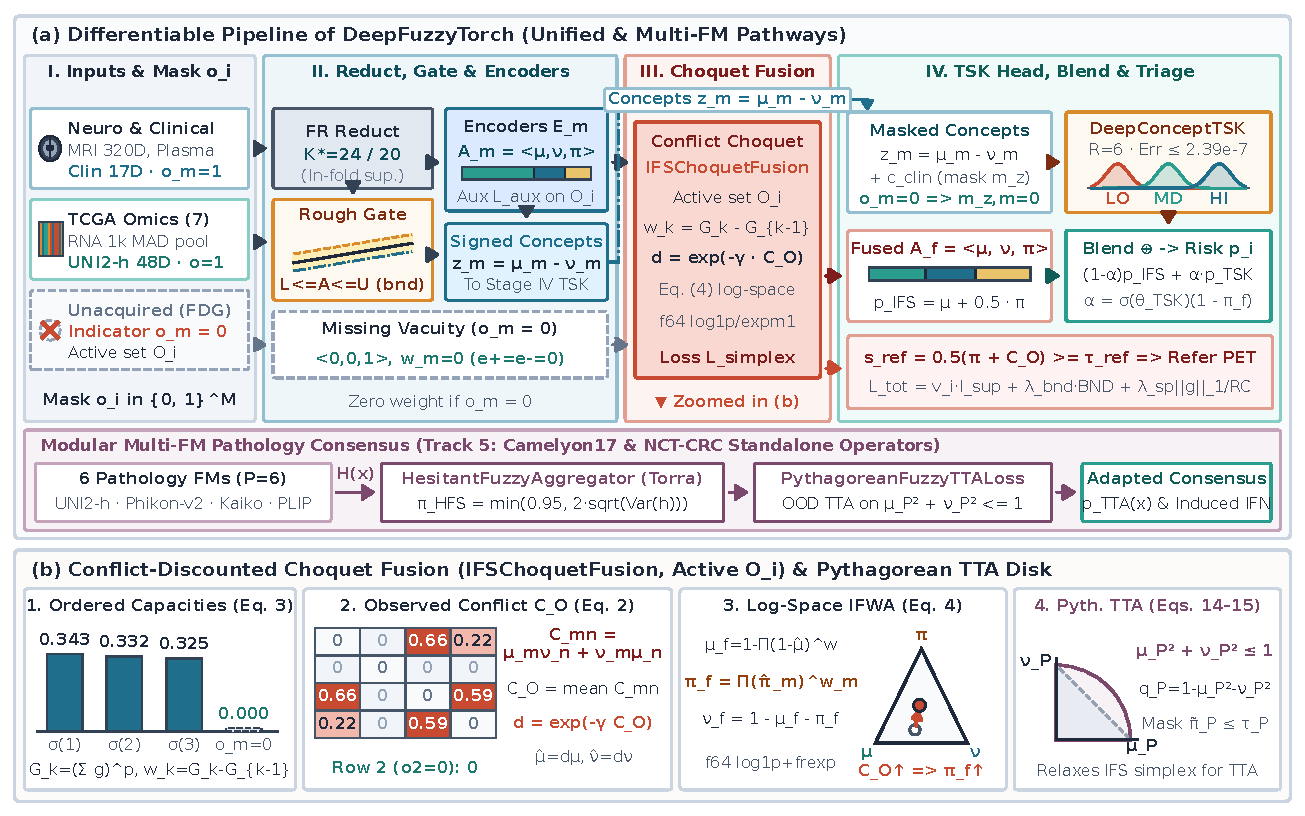
\includegraphics[width=\textwidth]{../figures/Fig0_System_Architecture_Overview.pdf}
    \caption{\textbf{System architecture and modular PyTorch operator graph of
    \texttt{DeepFuzzyTorch}.} \textbf{(a)} Four-stage multimodal pipeline: cohorts with binary
    observation indicators $\bm{o}_i \in \{0,1\}^M$ and active subsets $\mathcal{O}_i = \{m :
    o_{i,m}=1\}$ pass through in-fold MAD-standardized pointwise T-norm reduction
    (\texttt{FuzzyRoughFeatureReducer}, $K^*=24$ MRI ROIs; $K^*=20$ TCGA genes), unimodal
    simplex encoding (\texttt{IntuitionisticFuzzyEncoder}), soft-{\L}ukasiewicz boundary
    modulation (\texttt{FuzzyRoughAttentionGate}), conflict-discounted
    \texttt{IFSChoquetFusion} (or \texttt{HesitantFuzzyAggregator} +
    \texttt{PythagoreanFuzzyTTALoss}), and concept-masked \texttt{DeepConceptTSKHead} inference
    ($\bm{m}_{z,i}$, text reconstruction error $\le 2.39\times 10^{-7}$, exact Fold-0 error
    $2.384\times 10^{-7}$). \textbf{(b)} Mathematical mechanics of conflict-discounted
    \texttt{IFSChoquetFusion} (Eqs.~\eqref{eq:choquet_weights}--\eqref{eq:ifwa_closed}) and the
    unsupervised Pythagorean TTA disk (Eqs.~\eqref{eq:pfs_tta_base}--\eqref{eq:pfs_tta}).}
    \label{fig:system_architecture}
\end{figure*}

\subsection{Intuitionistic Fuzzy Encoding and Conflict-Discounted Choquet Fusion}

\begin{definition}[Differentiable Intuitionistic Fuzzy Tensor]
\label{def:ifn}
Let $\Delta_{\text{IFS}} = \{(\mu, \nu, \pi) \in [0,1]^3 : \mu + \nu + \pi = 1\}$ denote the
Atanassov intuitionistic fuzzy simplex \cite{atanassov1986intuitionistic}. For each modality $m
\in \{1,\dots,M\}$ under binary observation indicator $o_m \in \{0,1\}$, let $u_m \in
\mathbb{R}^{D_m^{\text{enc}}}$ denote the sanitized encoder input ($u_m = \tilde{x}_m = o_m
\cdot \operatorname{nan\_to\_num}(x_m) \in \mathbb{R}^{D_m}$ when
\texttt{IntuitionisticFuzzyEncoder} $\mathcal{E}_m$ is invoked standalone, or $u_m =
[\tilde{t}_m \,\|\, \hat{x}_m] \in \mathbb{R}^{d_e + D_m}$ concatenating the refined token
$\tilde{t}_m$ and gated input $\hat{x}_m$ in the multimodal pipeline). Combining a two-layer
GELU backbone $h_m(u_m) \in \mathbb{R}^{d_h}$ with direct linear residual skip projections
$s_m^+(u_m), \allowbreak s_m^-(u_m)$ (which preserve 1D and low-dimensional quantitative
biomarkers), $\mathcal{E}_m$ generates non-negative support evidence $e_m^+(u_m) = \allowbreak
o_m \operatorname{Softplus}\allowbreak(W_m^+ h_m(u_m) + b_m^+ + s_m^+(u_m)) \ge 0$, refutation
evidence $e_m^-(u_m) = \allowbreak o_m \operatorname{Softplus}\allowbreak(W_m^- h_m(u_m) +
b_m^- + s_m^-(u_m)) \ge 0$, and learnable scalar prior vacuity mass $\pi_m^{\text{prior}} =
\operatorname{Softplus}(\tau_{\pi,m}) + \epsilon_0 > 0$ ($\epsilon_0 = 10^{-4}$). The raw IFN
$\langle \mu_m^{\text{raw}}, \nu_m^{\text{raw}}, \pi_m^{\text{raw}} \rangle$ is projected onto
$\Delta_{\text{IFS}}$ via:
\begin{equation}
\label{eq:ifs_encoder}
\begin{aligned}
\mu_m^{\text{raw}}(x) &= \frac{e_m^+(u_m)}{e_m^+(u_m) + e_m^-(u_m) + \pi_m^{\text{prior}}}, \\
\nu_m^{\text{raw}}(x) &= \frac{e_m^-(u_m)}{e_m^+(u_m) + e_m^-(u_m) + \pi_m^{\text{prior}}}, \\
\pi_m^{\text{raw}}(x) &= 1 - \mu_m^{\text{raw}} - \nu_m^{\text{raw}} =
\frac{\pi_m^{\text{prior}}}{e_m^+ + e_m^- + \pi_m^{\text{prior}}},
\end{aligned}
\end{equation}
followed by optional fuzzy-rough certainty modulation $\mu_m =
\rho_m^{\text{FR}}\mu_m^{\text{raw}}, \allowbreak \nu_m = \rho_m^{\text{FR}}\nu_m^{\text{raw}},
\allowbreak \pi_m = 1 - \mu_m - \nu_m$ ($\rho_m^{\text{FR}} \in [0.75, 1.0]$;
$\rho_m^{\text{FR}} = 1$ in standalone encoding), so that $\mathcal{A}_m(x) = \langle \mu_m(x),
\nu_m(x), \pi_m(x)\rangle = \langle 0, 0, 1\rangle$ identically whenever $o_m = 0$. The
non-vacuity certainty mass of modality $m$ is $r_m(x) = 1 - \pi_m(x) = \mu_m(x) + \nu_m(x) \in
[0, 1]$ (lying strictly in $[0, 1)$ for real-arithmetic outputs of Eq.~\eqref{eq:ifs_encoder}
since $\pi_m^{\text{prior}} > 0 \implies \pi_m \ge \pi_m^{\text{raw}} > 0$).
\end{definition}

\begin{definition}[Conflict-Discounted Choquet Intuitionistic Fuzzy Aggregation]
\label{def:choquet}
Given $M$ modality IFNs $\{\mathcal{A}_m\}_{m=1}^M \subset \Delta_{\text{IFS}}$, let
$\mathcal{O} = \{m \in \{1,\dots,M\} : r_m > 0\}$ be the set of active modalities with strictly
positive non-vacuity mass and active indicator $a_m = \mathbb{I}(r_m > 0) = \mathbb{I}(\mu_m >
0 \lor \nu_m > 0)$ (for real-arithmetic outputs of Definition~\ref{def:ifn}, $a_m = o_m$ so
$\mathcal{O}$ coincides with the acquired set $\mathcal{A} = \{m : o_m = 1\}$; for general
standalone inputs on $\Delta_{\text{IFS}}$, $\mathcal{O} \subseteq \mathcal{A}$). When
$\mathcal{O} = \emptyset$, the fused output is $\mathcal{A}_{\text{fused}} = \langle 0, 0,
1\rangle$. When $|\mathcal{O}| \ge 1$, \texttt{IFSChoquetFusion} proceeds in three stages:
\begin{enumerate}[leftmargin=1.4em,itemsep=1pt]
    \item \textbf{Observed-Pair Evidential Conflict:} For each pair $(m, n)$, the
    cross-polarity contradiction mass is $C_{m,n} = \mu_m \nu_n + \nu_m \mu_n =
    \frac{1}{2}\big(r_m r_n - (\mu_m - \nu_m)(\mu_n - \nu_n)\big) \in [0, 1]$. For
    $|\mathcal{O}| \le 1$, $C_{\mathcal{O}} = 0$; for $|\mathcal{O}| \ge 2$, the average
    observed-pair conflict $C_{\mathcal{O}} \in [0, 1]$ is:
    \begin{equation}
    \label{eq:conflict_obs}
    C_{\mathcal{O}} = \frac{1}{|\mathcal{O}|(|\mathcal{O}|-1)} \sum_{\substack{m,n \in
    \mathcal{O}\\ m \neq n}} (\mu_m \nu_n + \nu_m \mu_n).
    \end{equation}
    \item \textbf{Certainty-Ordered Non-\allowbreak Additive Monotone Choquet Capacity
    Weights:} Let $\theta_m \in \mathbb{R}$ be learnable fuzzy density parameters with positive
    base density $g_m = \allowbreak \operatorname{Softplus}(\theta_m) + \allowbreak \epsilon_g
    > 0$ ($\epsilon_g = 10^{-3}$), and let $\eta \in \mathbb{R}$ parameterize the
    non-\allowbreak additive coalition exponent $p = \allowbreak \exp(\kappa \tanh(\eta)) \in
    (e^{-\kappa}, e^\kappa) \subset (0, \infty)$ ($\kappa = 0.35$; while
    Theorems~\ref{thm:closure}--\ref{thm:degeneration} hold for any $p > 0$). Sorting
    modalities in stable canonical descending order of active certainty $r_{\sigma(1)}
    a_{\sigma(1)} \ge \allowbreak r_{\sigma(2)} a_{\sigma(2)} \ge \allowbreak \dots \ge
    \allowbreak r_{\sigma(M)} a_{\sigma(M)}$ (ties resolved by canonical modality index order;
    all vacuous modalities with $r_m = 0$ placed at the tail), let $\bar{g}_{\sigma(k)} =
    \allowbreak \frac{g_{\sigma(k)} r_{\sigma(k)} a_{\sigma(k)}}{\sum_{j=1}^M g_{\sigma(j)}
    r_{\sigma(j)} a_{\sigma(j)}}$. Defining cumulative coalition capacities $G_k =
    (\sum_{j=1}^k \bar{g}_{\sigma(j)})^p$ with $G_0 = 0$, the certainty-ordered Choquet
    capacity increment weights (which for $p \neq 1$ are piecewise smooth on strict
    certainty-ordering chambers and defined at positive-certainty ties by the canonical index
    order) are:
    \begin{equation}
    \label{eq:choquet_weights}
    w_{\sigma(k)} = G_k - G_{k-1}, \qquad \forall k \in \{1,\dots,M\}.
    \end{equation}
    \item \textbf{Conflict-Discounted Capacity-Weighted Geometric-Hesitancy Aggregation
    (Hesitancy-Preserving IFWA):} For conflict penalty $\gamma \ge 0$, let $d = \exp(-\gamma
    C_{\mathcal{O}}) \in (0, 1]$ discount each modality's directional belief and disbelief into
    $\hat{\mu}_m = d\,\mu_m$, $\hat{\nu}_m = d\,\nu_m$, and $\hat{\pi}_m = 1 - d(\mu_m + \nu_m)
    \in [0, 1]$. Inspired by Xu and Yager's intuitionistic fuzzy multiplicative aggregation
    \cite{xu2006some,xu2007intuitionistic}, we apply capacity-weighted geometric pooling to $(1
    - \hat{\mu}_m)$ and $\hat{\pi}_m$ rather than $\hat{\nu}_m$ (so that whenever $\hat{\mu}_j
    < 1$ for all positive-weight active modalities and at least one positive-weight active
    modality has $\hat{\nu}_{m^*} > 0$, $\nu_{\text{fused}} =
    [\prod_{j\in\mathcal{O}}(1-\hat{\mu}_j)^{w_j}][1 - \prod_{j\in\mathcal{O}}(1 -
    \frac{\hat{\nu}_j}{1-\hat{\mu}_j})^{w_j}] > 0$, avoiding standard IFWA's $\nu_{\text{IFWA}}
    = \prod_m \hat{\nu}_m^{w_m} = 0$ zero-veto collapse when a single modality has $\hat{\nu}_m
    = 0$) to obtain $\mathcal{A}_{\text{fused}} = \langle \mu_{\text{fused}},
    \nu_{\text{fused}}, \pi_{\text{fused}} \rangle$:
    \begin{equation}
    \label{eq:ifwa_closed}
    \begin{aligned}
    \mu_{\text{fused}} &= 1 - \prod_{m=1}^M (1 - \hat{\mu}_m)^{w_m}, \\
    \pi_{\text{fused}} &= \prod_{m=1}^M (\hat{\pi}_m)^{w_m}, \\
    \nu_{\text{fused}} &= \prod_{m=1}^M (1 - \hat{\mu}_m)^{w_m} - \prod_{m=1}^M
    (\hat{\pi}_m)^{w_m}.
    \end{aligned}
    \end{equation}
\end{enumerate}
The expected diagnosis probability is the exported pignistic projection $P(y=1\mid x) =
\operatorname{clamp}(\mu_{\text{fused}} + \frac{1}{2}\pi_{\text{fused}}, 0, 1) = \frac{1}{2}(1
+ \mu_{\text{fused}} - \nu_{\text{fused}}) \in [0, 1]$. Half-precision
(\texttt{float16}/\texttt{bfloat16}) and \texttt{torch.autocast} modules and
\texttt{Intuitionistic\allowbreak Fuzzy\allowbreak Loss} execute internal evidence, simplex
normalization, fusion, and TSK paths in working precision (\texttt{float64}, or
\texttt{float32} on MPS) with fan-in-bounded backward casts and cancellation-free hesitancy
preservation. Meanwhile, straight-through $[\varepsilon_{\text{BCE}},
1-\varepsilon_{\text{BCE}}]$ clamping ($\varepsilon_{\text{BCE}}=10^{-4}$ for \texttt{float16},
$10^{-6}$ otherwise) applies strictly inside binary cross-entropy log evaluation and fallback
\texttt{torch.logit} conversion, preserving unclipped Brier and hesitancy targets on $[0,1]$
plus finite tail gradients.
\end{definition}

\begin{remark}[Piecewise Smoothness, Tie Blocks, Active-Set Jumps, \& Input Sanitization]
\label{rem:float64_choquet}
When $p \neq 1$, the Choquet weights in Eq.~\eqref{eq:choquet_weights} depend on the descending
permutation $\sigma$ of active certainties, so \texttt{IFSChoquetFusion} is $C^\infty$ on the
open interior of every strict certainty-ordering chamber for any fixed active set $\mathcal{O}$
(and globally $C^\infty$ on $(\Delta_{\text{IFS}}^\circ)^{|\mathcal{O}|}$ for fixed
$\mathcal{O} \neq \emptyset$ when $p = 1$, where $w_m = \bar{g}_m$). Across any multiway tied
positive-certainty block $B(r)=\{j\in\mathcal{O}: r_j=r>0\}$ ($|B(r)| \ge 2$) within
$\mathcal{H}_{\text{tie}} = \bigcup_{m<n\in\mathcal{O}} \{r_m = r_n > 0\}$, hesitancy
$\pi_{\text{fused}}$ remains continuous ($C^0$, piecewise $C^\infty$) on the fixed active-set
domain $(\Delta_{\text{IFS}} \setminus \{\langle 0,0,1\rangle\})^{|\mathcal{O}|}$. Meanwhile,
$(\mu_{\text{fused}}, \nu_{\text{fused}})$ is continuous across $B(r)$ iff either all $j\in
B(r)$ share equal $\mu_j$ or some active modality $m^*\in\mathcal{O}$ hits the absorbing vertex
$\hat{\mu}_{m^*} = d\mu_{m^*} = 1$ ($\mu_{m^*}=1$ and $\gamma C_{\mathcal{O}}=0$, forcing
$\mu_{\text{fused}}=1$ and $\nu_{\text{fused}}=0$ continuously). On the non-absorbing domain
$\{\hat{\mu}_m < 1\;\forall m\in\mathcal{O}\}$ (covering
$(\Delta_{\text{IFS}}^\circ)^{|\mathcal{O}|}$ and all $\gamma > 0$ with $C_{\mathcal{O}} > 0$),
unequal $\mu_m \neq \mu_n$ inside $B(r)$ always induce a finite capacity-swap jump ($\delta
\neq 0$ for $p \neq 1$) in $\mu_{\text{fused}}$ and $\nu_{\text{fused}}$, which
\texttt{IFSChoquetFusion} resolves deterministically via stable descending sorting preserving
canonical modality index order. Across the active-set transition $r_m : 0 \to \epsilon > 0$,
when $C_{\mathcal{O}} = 0$ (including $|\mathcal{O}| = 1 \to 2$) $d(\mathcal{C}_{\mathcal{O}})$
varies continuously, as do fused outputs provided the
pre-existing certainty ordering or equal-$\mu_j$ tie-block structure in $\mathcal{O}$ is
preserved; when $|\mathcal{O}| \ge 2$
with non-zero active conflict $C_{\mathcal{O}} > 0$, enlarging $|\mathcal{O}|$ changes the
denominator $|\mathcal{O}|(|\mathcal{O}|-1)$ in Eq.~\eqref{eq:conflict_obs}, producing a
$\gamma$-independent denominator jump in $C_{\mathcal{O}}$ and a uniform
$|\Delta d|=O(\gamma/|\mathcal{O}|)$ jump in $d(\mathcal{C}_{\mathcal{O}})$ for
$\gamma\ge0$, independently of the certainty ordering. For fused
outputs, the $O_\delta(\gamma/|\mathcal{O}|)$ bound holds on each compact interior set
$\{r_m \le 1-\delta\}^{|\mathcal{O}|}$ ($\delta>0$), provided the pre-existing certainty
ordering or equal-$\mu_j$ tie-block structure among active modalities in $\mathcal{O}$ is
preserved. A simultaneous reversal of a pre-existing unequal-$\mu$ tie at $p\ne1$ adds a
finite capacity-swap jump even at $\gamma=0$. Under the same ordering proviso, at closed
boundary vertices $r_j=1$ with
$C_{\mathcal{O}} > 0$, letting $W_\pi = \sum_{j \in \mathcal{O}: r_j=1} w_j \in (0, 1]$ and
$W_\mu = \sum_{j \in \mathcal{O}: \mu_j=1} w_j \in [0, 1)$ gives $|\Delta \pi_{\text{fused}}| =
\Theta(\gamma^{W_\pi})$, $|\Delta \mu_{\text{fused}}| = \Theta(\gamma^{W_\mu})$ if $W_\mu > 0$
else $O_{\delta_\mu}(\gamma/|\mathcal{O}|)$, $|\Delta \nu_{\text{fused}}| =
\Theta(\gamma^{W_*})$ whenever $W_* < 1$ (with guaranteed non-cancellation $A_\mu > A_\pi > 0$
at $W_\mu = W_\pi \in (0, 1)$), and $\|\Delta \mathcal{A}_{\text{fused}}\|_\infty =
\Theta(\gamma^{W_*})$ as $\gamma \to 0^+$ with $W_* = W_\mu$ if $W_\mu > 0$ else $W_\pi \in (0,
1]$ (sublinear Hölder whenever $W_* < 1$). Setting $\gamma=0$ leaves $d \equiv 1$ and removes
these discount-induced fused-output discontinuities, while Eq.~\eqref{eq:ifs_encoder} in
Definition~\ref{def:ifn} guarantees $\mathcal{O}=\mathcal{A}$ in real arithmetic at fixed
$\bm{o}_i$. Because Eq.~\eqref{eq:ifwa_closed} pools $(1-\hat{\mu}_m)$ and $\hat{\pi}_m$
geometrically, closed boundary vertices satisfy $\hat{\mu}_m = 1 \implies \mu_{\text{fused}}=1$
whereas $\hat{\nu}_m = 1$ ($\hat{\mu}_m=0,\hat{\pi}_m=0$) collapses $\pi_{\text{fused}}$ to $0$
without zero-vetoing $(1-\hat{\mu}_j)$ across $j \neq m$. For all acquired encoder outputs
($o_m=1$) of
Definition~\ref{def:ifn}, $\pi_m^{\text{prior}} > 0$ keeps every $\mathcal{A}_m$ strictly
inside the interior ($\hat{\mu}_m, \hat{\nu}_m < 1, \hat{\pi}_m > 0$), avoiding boundary
vetoes. For standalone callers passing malformed inputs (\texttt{NaN}, $\pm\infty$, negative
entries, $\mu_m+\nu_m>1$, or mismatched $\pi_m$), \texttt{\_sanitize\_input\_ifn\_f64} radially
projects $(\mu_m,\nu_m)$ onto $\Delta_{\text{IFS}}$ and recomputes $\pi_m$ across both
$|\mathcal{O}|=1$ and $|\mathcal{O}|\ge 2$ branches while acting as the identity on valid
closed-simplex inputs. In working precision (\texttt{float64} on CPU/CUDA, or \texttt{float32}
on MPS), \texttt{IFSChoquetFusion} rescales $r_m$ via \texttt{frexp}/\texttt{ldexp} so $\max_m
r_m \in [0.5, 1.0)$, passes valid $|\mathcal{O}|=1$ inputs through identically with simplex
tangent backward gradient $d\pi = -d\mu - d\nu$, and enforces a working-precision pre-log cap
($1 - 2^{-53}$ in \texttt{float64}; $1 - 2^{-24}$ in \texttt{float32}) on $\hat{\mu}_m$ and
$q_m = \hat{\nu}_m/(1-\hat{\mu}_m)$ before \texttt{log1p} on interior inputs while exact
boundary vertices use dedicated \texttt{any\_mu\_one}/\texttt{any\_pi\_zero} branches. Interior
products accumulate in canonical descending-$r_{\sigma(k)}$ working-precision log-space using
\texttt{log1p}/\texttt{expm1} and the cancellation-free factorization $\hat{\pi}_m = (1 -
\hat{\mu}_m)(1 - q_m)$ with subnormal power-of-two rescaling (below $10^{-300}$ in
\texttt{float64}).
\end{remark}

\begin{theorem}[Intuitionistic Simplex Closure and Fixed-$\mathcal{O}$ Piecewise Smoothness]
\label{thm:closure}
For any input collection $\{\mathcal{A}_m\}_{m=1}^M \subset \Delta_{\text{IFS}}$ with
$|\mathcal{O}| \ge 1$ (and any arbitrary inputs radially sanitized onto $\Delta_{\text{IFS}}$
inside \texttt{IFSChoquetFusion}), any exponent $p > 0$, and any $\gamma \ge 0$, the Choquet
weights in Eq.~\eqref{eq:choquet_weights} satisfy $w_m \ge 0$ and $\sum_{m=1}^M w_m = 1$, and
the fused triplet $\mathcal{A}_{\text{fused}}$ in Eq.~\eqref{eq:ifwa_closed} satisfies
intuitionistic closure $\mu_{\text{fused}} + \nu_{\text{fused}} + \pi_{\text{fused}} = 1$ with
$\mu_{\text{fused}}, \nu_{\text{fused}}, \pi_{\text{fused}} \in [0, 1]$ across
$\Delta_{\text{IFS}}$ ($\pi_{\text{fused}} > 0$ on the encoder interior $\hat{\pi}_m > 0$).
Moreover, for any fixed active set $\mathcal{O}$, $\mathcal{F}_{\text{IFC}}$ is $C^\infty$ on
$\big(\Delta_{\text{IFS}}^\circ\big)^{|\mathcal{O}|} \setminus \mathcal{H}_{\text{tie}}$
(globally $C^\infty$ at $p=1$ for fixed $\mathcal{O}$) and preserves $C^0$ continuity of
$\pi_{\text{fused}}$ across multiway tie blocks $B(r)$ in $\mathcal{H}_{\text{tie}}$ on
$(\Delta_{\text{IFS}} \setminus \{\langle 0,0,1\rangle\})^{|\mathcal{O}|}$. On the
non-absorbing domain $\{\hat{\mu}_m < 1\;\forall m\in\mathcal{O}\}$ for $p \neq 1$,
$(\mu_{\text{fused}}, \nu_{\text{fused}})$ is continuous across $B(r)$ iff $\mu_j$ is constant
on $B(r)$ (with continuous absorbing limit $\mu_{\text{fused}}=1$ whenever some active modality
satisfies $\hat{\mu}_{m^*}=1$), resolving unequal-$\mu$ capacity-swap jumps deterministically
by canonical index tie-breaking. Across an active-set transition $r_m : 0 \to \epsilon > 0$,
$d$ is continuous across $C_{\mathcal{O}}=0$ transitions (including
$|\mathcal{O}|=1 \to 2$), as are fused outputs under the ordering condition below. For
$|\mathcal{O}| \ge 2$ with $C_{\mathcal{O}} > 0$, the conflict exhibits a
$\gamma$-independent denominator jump alongside a uniform
$|\Delta d|=O(\gamma/|\mathcal{O}|)$ jump in $d(\mathcal{C}_{\mathcal{O}})$ for
$\gamma\ge0$, independently of ordering, inducing an
interior $O_\delta(\gamma/|\mathcal{O}|)$ fused-output jump on each $\{r_m \le
1-\delta\}^{|\mathcal{O}|}$ ($\delta>0$), provided the pre-existing certainty ordering or
equal-$\mu_j$ tie-block structure among active modalities in $\mathcal{O}$ is preserved. A
simultaneous reversal of a pre-existing unequal-$\mu$ tie at $p\ne1$ adds the finite
capacity-swap jump even at $\gamma=0$. Under the same ordering proviso, closed-boundary jumps
$|\Delta \pi_{\text{fused}}|
= \Theta(\gamma^{W_\pi})$, $|\Delta \nu_{\text{fused}}| = \Theta(\gamma^{W_*})$ ($W_* < 1$),
and $\|\Delta \mathcal{A}_{\text{fused}}\|_\infty = \Theta(\gamma^{W_*})$ as $\gamma \to 0^+$
($W_\pi, W_* \in (0, 1]$, sublinear Hölder whenever $< 1$) when active boundary vertices
$r_j=1$ appear.
\end{theorem}

\begin{theorem}[Algebraic Missing-Modality Vacuity Invariance]
\label{thm:degeneration}
Suppose modality subset $\mathcal{M}_{\text{miss}} \subset \{1,\dots,M\}$ is unacquired ($o_k =
0 \implies \mathcal{A}_k = \langle 0, 0, 1\rangle$ for all $k \in \mathcal{M}_{\text{miss}}$),
let $\mathcal{A} = \{1,\dots,M\} \setminus \mathcal{M}_{\text{miss}}$ be the non-empty acquired
subset, and let $\mathcal{O} = \{m \in \mathcal{A} : r_m > 0\} \subseteq \mathcal{A}$ be the
active non-vacuous subset (with $\mathcal{O} = \mathcal{A}$ for real-arithmetic outputs of
Definition~\ref{def:ifn}). Then for the standalone \texttt{IFSChoquetFusion} operator under any
conflict penalty $\gamma \ge 0$, any shared restricted fuzzy densities
$\{\theta_m\}_{m\in\mathcal{A}}$, any Choquet exponent $p > 0$, and regardless of the insertion
indices occupied by $\mathcal{M}_{\text{miss}}$ preserving the relative index order of
$\mathcal{A}$ (or for arbitrary permutations when active certainties
$\{r_m\}_{m\in\mathcal{O}}$ are distinct or $p=1$): (i) $w_k = 0$ for all $k \in
\mathcal{M}_{\text{miss}}$ (and any $k \in \mathcal{A}\setminus\mathcal{O}$), (ii)
$C_{\mathcal{O}}(\{\mathcal{A}_m\}_{m=1}^M) =
C_{\mathcal{O}}(\{\mathcal{A}_m\}_{m\in\mathcal{A}})$, and (iii) the $M$-modality operator is
algebraically invariant to $\mathcal{M}_{\text{miss}}$:
\begin{equation}
\begin{aligned}
\operatorname{IFSChoquetFusion}\big(\{\mathcal{A}_m\}_{m=1}^M\big) \\
= \operatorname{IFSChoquetFusion}\big(\{\mathcal{A}_m\}_{m\in\mathcal{A}}\big),
\end{aligned}
\end{equation}
where canonical descending-$r_m$ float64 accumulation achieves $0.00 \times 10^0$ maximum
absolute deviation across all vacuity positions.
\end{theorem}

\begin{corollary}[End-to-End Missing-Modality Padding-Value and Submodel Invariance]
\label{cor:e2e_vacuity}
In \texttt{UnifiedDeepFuzzyModel} with \texttt{disable\_vacuity\_mask=False}, every unimodal
module ($\mathcal{G}_m^{\text{feat}}, \mathcal{P}_m, \texttt{FuzzyRoughAttentionGate}_m,
\mathcal{E}_m$) operates strictly unimodally and masks $o_{i,m}=0$ to $\mathcal{A}_{i,m} =
\langle 0,0,1\rangle$ ($z_{i,m}=0, r_{i,m}=0$), while \texttt{DeepConceptTSKHead} applies the
binary concept mask $\bm{m}_{z,i} \in \{0,1\}^C$ combining modality indicators and optional
elementwise \texttt{clinical\_\allowbreak concept\_\allowbreak masks} ($m_{z,i,c}=0$ for
missing
modalities, unobserved clinical sub-indicators, and any zero-padded trailing concept slots) in
Eqs.~\eqref{eq:tsk_firing}--\eqref{eq:tsk_consequent}. Consequently, (i) the end-to-end output
$(p_i, \mathcal{A}_{\text{fused},i}, C_{\mathcal{O},i}, \bm{w}_i)$ is strictly invariant
($0.00$
fixed-width deviation) to arbitrary finite or \texttt{NaN}/\texttt{Inf} values placed in
$\{x_{i,k}\}_{k\in\mathcal{M}_{\text{miss}}}$. Optional elementwise masks also give exact
$0.00$ invariance to arbitrary fill or perturbation values in masked entries of the
\texttt{clinical\_\allowbreak concepts} tensor passed to \texttt{DeepConceptTSKHead},
holding upstream modality encoder inputs $\{x_{i,m}\}$ fixed (or when shared raw clinical
variables are simultaneously masked in $x_{i,\text{Clin}}$). Moreover, (ii) when
\texttt{DeepConceptTSKHead} shares identical restricted rule parameters on observed concepts
($m_{z,i,c}=1$), the $M$-modality model output is algebraically equivalent in exact real
arithmetic to the restricted $(|\mathcal{A}|, |\mathcal{C}_{\text{obs},i}|)$-submodel, matching
its predicted probability within reduction-order rounding scaling proportionally with parameter
magnitude ($\le 10^{-7}$ in the Track-0 benchmark audit; $\le 10^{-6}$ across tested
default-scale
variable-width float32 unit checks, and $< 10^{-14}$ in float64 on tested scales).
\end{corollary}

\begin{theorem}[Partial-Order Monotonicity and Coupled Conflict Boundary]
\label{thm:monotonicity}
With respect to the Atanassov partial order $\langle \mu, \nu, \pi\rangle \preceq_{\text{IFS}}
\langle \mu', \nu', \pi'\rangle \iff \mu \le \mu' \text{ and } \nu \ge \nu'$ along
constant-certainty contours $\nu_m = r_m - \mu_m$ ($r_m = 1 - \pi_m \in (0, 1)$), suppose all
active modalities $k \in \mathcal{O}$ satisfy $\hat{\pi}_k = 1 - d r_k > 0$ (guaranteed by
Definition~\ref{def:ifn}). Let $F_\mu(\bm{\mu}; \bm{r}, d) = 1 - \prod_{j\in\mathcal{O}}(1 -
d\mu_j)^{w_j(\bm{r})}$ and $F_\nu = 1 - F_\mu - \prod_{j\in\mathcal{O}}(1 - d
r_j)^{w_j(\bm{r})}$ denote the aggregation maps at fixed certainty vector $\bm{r}$ and frozen
conflict discount $d \in (0, 1]$. Then for every active modality $m \in \mathcal{O}$ ($w_m >
0$):
\begin{equation}
\left.\frac{\partial F_\mu}{\partial \mu_m}\right|_{\bm{r}, d} = \left.\frac{\partial
F_\nu}{\partial \nu_m}\right|_{\bm{r}, d} = w_m d \frac{1 - \mu_{\text{fused}}}{1 -
\hat{\mu}_m} > 0,
\end{equation}
whereas under coupled conflict $C_{\mathcal{O}}(\bm{\mu})$ ($|\mathcal{O}|\ge 2$),
$\frac{d\mu_{\text{fused}}}{d\mu_m}\big|_{\bm{r},\bm{\mu}_{-m}} =
(1-\mu_{\text{fused}})d\big[\frac{w_m}{1-d\mu_m} - \gamma\frac{\partial
C_{\mathcal{O}}}{\partial \mu_m}\sum_{j\in\mathcal{O}}\frac{w_j\mu_j}{1-d\mu_j}\big]$ with
$\frac{\partial C_{\mathcal{O}}}{\partial \mu_m} =
\frac{2}{|\mathcal{O}|(|\mathcal{O}|-1)}\sum_{j\in\mathcal{O}\setminus\{m\}}(\nu_j - \mu_j)$,
remaining strictly positive whenever $\gamma\frac{\partial C_{\mathcal{O}}}{\partial
\mu_m}\sum_{j\in\mathcal{O}}\frac{w_j\mu_j}{1-d\mu_j} < \frac{w_m}{1-d\mu_m}$ (and for all
$\gamma\ge 0$ when $\sum_{j\neq m}(\nu_j-\mu_j)\le 0$), whereas strong opposing refutation at
large $\gamma$ allows conflict discounting to outweigh unimodal support growth. Furthermore,
when active modalities are identical ($\tilde{\alpha}_m = \langle \mu_0, \nu_0, \pi_0\rangle$
for all $m\in\mathcal{O}$), self-pair cross-polarity contradiction equals
$C_{\mathcal{O}} = 2\mu_0\nu_0 > 0$ whenever $\mu_0,\nu_0 > 0$, so exact idempotency holds at
$\gamma=0$ (or crisp/unipolar agreement $\mu_0\nu_0=0$), while $\gamma > 0$ attenuates mixed
inputs proportionally to $2\mu_0\nu_0$.
\end{theorem}

\begin{theorem}[Conflict-Driven Epistemic Hesitancy Inflation]
\label{thm:conflict}
For any observed interior configuration $|\mathcal{O}| \ge 2$ in \texttt{IFSChoquetFusion} with
$\gamma > 0$ and $\sum_{m\in\mathcal{O}} w_m r_m > 0$, holding the modality non-vacuity
certainty masses $r_m = 1 - \pi_m = \mu_m + \nu_m \in (0, 1)$ fixed (so that $\partial w_m /
\partial C_{\mathcal{O}} = 0$), the fused epistemic hesitancy $\pi_{\text{fused}}$ is strictly
monotonically increasing with respect to the cross-modal conflict $C_{\mathcal{O}}$:
\begin{equation}
\frac{\partial \ln \pi_{\text{fused}}}{\partial C_{\mathcal{O}}} = \gamma \sum_{m \in
\mathcal{O}} w_m \frac{\hat{\mu}_m + \hat{\nu}_m}{\hat{\pi}_m} > 0.
\end{equation}
\end{theorem}

All complete proofs of Theorems~\ref{thm:closure}--\ref{thm:rough} and
Corollary~\ref{cor:e2e_vacuity} are provided in Appendix~\ref{app:proofs}.

\subsection{Hesitant Fuzzy Multi-Foundation-Model Consensus}

\begin{definition}[Median-Concordant Hesitant Fuzzy Aggregator]
\label{def:hfs}
When $P$ heterogeneous pathology foundation models produce a membership prediction vector
$\bm{h}(x) = (h_1(x),\dots,h_P(x)) \in (0,1)^P$ forming a hesitant fuzzy element
$\mathcal{H}(x) = \{h_p(x)\}_{p=1}^P \subset (0,1)$, uniform averaging is vulnerable to outlier
experts degraded by staining or scanner shifts. Following Torra's Hesitant Fuzzy Set (HFS)
formalism and hesitant dispersion measures
\cite{torra2010hesitant,xia2012entropy,liao2013vikor}, \texttt{Hesitant\allowbreak
Fuzzy\allowbreak Aggregator} clamps inputs to $[10^{-6}, 1-10^{-6}]$ and quantifies inter-model
epistemic dispersion via population variance $\operatorname{Var}_p(h_p(x)) =
\frac{1}{P}\sum_{p=1}^P (h_p(x) - \bar{h}(x))^2$: $\pi_{\text{HFS}}^{\text{raw}}(x) =
\min\!\big(1, 2\sqrt{\operatorname{Var}_p(h_p(x)) + 10^{-12}}\big)$. The induced IFN hesitancy
is capped at $\pi_{\text{HFS}}(x) = \min\!\big(0.95, 2\sqrt{\operatorname{Var}_p(h_p(x)) +
10^{-12}}\big)$ to preserve non-degenerate support and refutation mass. Consensus weights are
computed using PyTorch's lower-median order statistic $\operatorname{median}(\mathcal{H}(x))$
(\texttt{torch.median}, returning the 3rd sorted value when $P=6$):
\begin{equation}
\label{eq:hfs_weights}
\begin{aligned}
\omega_p(x) = \operatorname{Softmax}_p\Big(&\alpha_p + \beta_{\text{cert}} |2h_p(x)-1| \\
&- \kappa_{\text{med}} \big|h_p(x) - \operatorname{median}(\mathcal{H}(x))\big|\Big),
\end{aligned}
\end{equation}
where $\alpha_p \in \mathbb{R}$ is a learnable expert reliability prior, $\beta_{\text{cert}} =
\operatorname{Softplus}(\tau_{\text{cert}})$ ($\tau_{\text{cert}} \in \mathbb{R}$ learnable),
and $\kappa_{\text{med}} > 0$ (\texttt{concordance\_kappa}, default $3.5$; $\kappa_{\text{med}}
= 2.6$ in Track~5) is a fixed positive scalar hyperparameter that suppresses outlier experts
deviating from the ensemble median. This produces consensus membership $\mu_{\text{HFS}}(x) =
\sum_{p=1}^P \omega_p(x) h_p(x)$ and induced IFN $\langle (1-\pi_{\text{HFS}})\mu_{\text{HFS}},
(1-\pi_{\text{HFS}})(1-\mu_{\text{HFS}}), \pi_{\text{HFS}}\rangle \in \Delta_{\text{IFS}}$.
\end{definition}

\subsection{Soft-\texorpdfstring{{\L}}{L}ukasiewicz Differentiable Fuzzy-Rough Bottleneck and
Pointwise T-Norm Reduction}

\begin{definition}[Blended Soft-{\L}ukasiewicz Fuzzy-Rough Approximation]
\label{def:fuzzy_rough}
In \texttt{DifferentiableFuzzyRoughLayer}, given $N$ tokens with active mask $t_i \in \{0,1\}$,
valid neighborhood $V_i = \{j \in \{1,\dots,N\} : \max(t_j, \delta_{ij}) = 1\}$ ($i \in V_i$),
linear projections $z_i = W_{\text{proj}} x_i + b_{\text{proj}} \in \mathbb{R}^{d_h}$, and
positive bandwidth $\sigma_\theta = \operatorname{Softplus}(\tilde{\sigma}_\theta) + 0.1 > 0$,
the reflexive $L_1$ similarity kernel is $R_\theta(x_i, x_j) = \max(t_i t_j,
\delta_{ij})\exp\!\big(-\frac{1}{d_h \sigma_\theta}\sum_{d=1}^{d_h} |z_{i,d} - z_{j,d}|\big)
\in [0, 1]$ with $R_\theta(x_i, x_i) = 1$. For fuzzy concept membership $A(x_j) \in [0, 1]$,
the {\L}ukasiewicz implicator is $\psi_{ij} = \operatorname{clamp}(1 - R_\theta(x_i,x_j) +
A(x_j), 0, 1)$ and the {\L}ukasiewicz t-norm is $\phi_{ij} =
\operatorname{clamp}(R_\theta(x_i,x_j) + A(x_j) - 1, 0, 1)$. Over $j \in V_i$, shift-stabilized
softmin/softmax weights $p_{ij}^- = \frac{\exp(-(\psi_{ij} - \min_{k\in
V_i}\psi_{ik})/\tau)}{\sum_{k\in V_i} \exp(-(\psi_{ik} - \min_{l\in V_i}\psi_{il})/\tau)}$ and
$p_{ij}^+ = \frac{\exp((\phi_{ij} - \max_{k\in V_i}\phi_{ik})/\tau)}{\sum_{k\in V_i}
\exp((\phi_{ik} - \max_{l\in V_i}\phi_{il})/\tau)}$ ($\tau_{\text{eff}} = \max(\tau,
10^{-30})$, evaluated in working precision (\texttt{float64}, or \texttt{float32} on MPS) when
$\tau_{\text{eff}} < 10^{-4}$, in half precision, or under \texttt{torch.autocast}) are blended
with hard extrema via $\beta \in [0, 1]$ ($\beta = 0.5$ default) to form
$\underline{R}_{\text{raw}}(A)(x_i) = (1-\beta)\min_{j\in V_i} \psi_{ij} + \beta \sum_{j=1}^N
p_{ij}^- \psi_{ij}$ and $\overline{R}_{\text{raw}}(A)(x_i) = (1-\beta)\max_{j\in V_i} \phi_{ij}
+ \beta \sum_{j=1}^N p_{ij}^+ \phi_{ij}$. Anchoring against the reflexive self-pair $j=i$
($\psi_{ii}=\phi_{ii}=A(x_i)$) defines the projected bounds:
\begin{equation}
\label{eq:fuzzy_rough_bounds}
\begin{aligned}
\underline{R}_\tau(A)(x_i) &= \min\!\big(\underline{R}_{\text{raw}}(A)(x_i),\; A(x_i)\big), \\
\overline{R}_\tau(A)(x_i) &= \max\!\big(\overline{R}_{\text{raw}}(A)(x_i),\; A(x_i)\big).
\end{aligned}
\end{equation}
\end{definition}

For single-instance inference without cross-modality or cross-batch coupling,
\texttt{FuzzyRough\allowbreak AttentionGate} applies positive feature relevance weights
$w_\theta = \operatorname{Softplus}(\tilde{w}_\theta) > 0$ before projecting into $G=5$
internal granular memberships $\{a_{b,m,g}\}_{g=0}^{G-1} \subset (0,1)$ anchored at $A_{b,m} =
o_{b,m} a_{b,m,0}$ with similarity $R_{b,m,g} = \exp(-\gamma_{\text{FR}}|a_{b,m,g}-A_{b,m}|)$
($\gamma_{\text{FR}} = 0.25\,\sigma(\tilde{\gamma}_{\text{FR}}) + 0.05$) and learnable $\beta =
\sigma(\beta_{\text{raw}}) \in (0,1)$ ($\tau = 0.15$ in \texttt{UnifiedDeepFuzzyModel}; $\tau =
0.06$ in Track~0 verification), modulating unimodal certainty via $\rho_m^{\text{FR}} =
\operatorname{clamp}(1 - 0.12\,\operatorname{BND}_R(A)_m, 0.75, 1.0)$ while masking $o_{b,m}=0$
outputs to $0$.

The neural \texttt{DifferentiableFuzzyRoughLayer} and unimodal
\texttt{FuzzyRoughAttentionGate} are end-to-end differentiable in PyTorch. The discrete
\texttt{FuzzyRoughFeatureReducer} is an offline tensor-accelerated pointwise T-norm
forward-greedy selector; its selection step is not end-to-end gradient-differentiable.
For offline in-fold attribute reduction on high-dimensional modalities ($D=320$ ADNI MRI
features and $D=1,000$ TCGA RNA-Seq genes), \texttt{FuzzyRough\allowbreak Feature\allowbreak
Reducer} subsamples batches exceeding \texttt{max\_\allowbreak samples} ($4,096$) via
class-stratified sampling without replacement and avoids dimensionality-induced distance
concentration by standardizing each coordinate via training-fold median and Gaussian-consistent
dispersion $\operatorname{MAD}_k = 1.4826\,\operatorname{med}_i|x_{i,k}-\operatorname{med}_k|$
with robust scale $s_k = 4\cdot\operatorname{MAD}_k$ whenever $\operatorname{MAD}_k >
10^{-6}$ ($4\cdot\operatorname{SD}_k$ fallback when $\operatorname{MAD}_k \le 10^{-6} <
\operatorname{SD}_k$, and $s_k = 4.0$ when both $\operatorname{MAD}_k \le 10^{-6}$ and
$\operatorname{SD}_k \le 10^{-6}$, including constant or all-missing columns):
$\tilde{x}_{i,k} = (x_{i,k} - \operatorname{med}_k)/s_k$. Defining the 1D exponential Laplace
similarity $R_{\{k\}}(x_i,x_j) = \exp(-|\tilde{x}_{i,k}-\tilde{x}_{j,k}|/\sigma)$
($\sigma=0.85$) and the classical Pawlak--Dubois--Prade pointwise minimum T-norm
$R_{\mathcal{B}}(x_i,x_j) = \min_{k\in\mathcal{B}} R_{\{k\}}(x_i,x_j)$ (with optional product
and {\L}ukasiewicz T-norms), we evaluate all non-self pairs $V_i = \{j \in \{1,\dots,N\} : j
\neq i\}$ ($|V_i|=N-1$). Specifically, the crisp-decision {\L}ukasiewicz implicator
$I_{\mathcal{B}}(i,j) = \min(1, 1 - R_{\mathcal{B}}(x_i,x_j) + \mathbb{I}[y_i = y_j]) \in
[0,1]$ equals $1$ when $y_j = y_i$ and $1 - R_{\mathcal{B}}(x_i,x_j)$ when $y_j \neq y_i$.
Replacing the hard infimum over $V_i$ with the shifted LogSumExp soft-infimum ($\tau =
\tau_{\text{reducer}} = 0.08$):
\begin{equation}
\label{eq:reducer_softmin}
\begin{aligned}
I_{\min,i} &= \min_{j\in V_i} I_{\mathcal{B}}(i,j), \\
\underline{R}_{\mathcal{B},\tau}(D_{y_i})(x_i) &= \min\!\Big(1,\; I_{\min,i} \\
&\quad - \tau\ln\!\Big[\frac{1}{|V_i|}\sum_{j\in V_i} e^{-(I_{\mathcal{B}}(i,j) -
I_{\min,i})/\tau}\Big]\Big),
\end{aligned}
\end{equation}
clamped to $[0,1]$, yields monotonic positive dependency $\gamma_{\mathcal{B}}(D) =
\frac{1}{N}\sum_{i=1}^N \underline{R}_{\mathcal{B},\tau}(D_{y_i})(x_i) \in [0,1]$ and
complementary boundary $\operatorname{BND}_{\mathcal{B}}(D) = 1 - \gamma_{\mathcal{B}}(D)$.
Because $\gamma_{\mathcal{B}}(D)$ grows monotonically with $|\mathcal{B}|$ even under random
labels, \texttt{FuzzyRoughFeatureReducer} computes a label-permutation null curve
$\gamma_{\mathcal{B}}^{\text{null}}(D)$ ($n_{\text{perm}}=8$ in our ADNI/TCGA benchmarks; class
default $12$) and performs forward-greedy maximization of normalized excess dependency
$\widehat{\Delta}\gamma_{\mathcal{B}}(D) = \frac{\gamma_{\mathcal{B}}(D) -
\gamma_{\mathcal{B}}^{\text{null}}(D)}{\max(10^{-6}, 1 -
\gamma_{\mathcal{B}}^{\text{null}}(D))} + 10^{-4}\gamma_{\mathcal{B}}(D)$. Candidate scores are
aggregated across $5$ (ADNI MRI) and $8$ (TCGA RNA-Seq) stratified without-replacement
subsample views ($85\%$ per view below \texttt{max\_\allowbreak samples}) up to budget
$K^*$ ($K^*=24$ on ADNI MRI, $92.50\%$ compression; $K^*=20$ on TCGA RNA-Seq, $98.00\%$
compression), alongside a backward minimality check down to size $1$.

\begin{theorem}[Differentiable Fuzzy-Rough Inclusion and Pointwise T-Norm Reduction Guarantees]
\label{thm:rough}
\textbf{(Part I: Neural Inclusion Envelope)} For any reflexive similarity kernel $R_\theta(x_i,
x_i) = 1$, target membership $A(x_i) \in [0, 1]$, blend $\beta \in [0, 1]$, and $\tau > 0$,
Eq.~\eqref{eq:fuzzy_rough_bounds} strictly satisfies
\begin{equation}
0 \le \underline{R}_\tau(A)(x_i) \le A(x_i) \le \overline{R}_\tau(A)(x_i) \le 1,
\end{equation}
so $\operatorname{BND}_R(A)(x_i) = \overline{R}_\tau(A)(x_i) - \underline{R}_\tau(A)(x_i) \ge
0$ is everywhere non-negative and piecewise continuously differentiable a.e. \textbf{(Part II:
Pointwise T-Norm Monotonicity)} In \texttt{FuzzyRoughFeatureReducer}, for every nested
attribute pair $\emptyset \neq \mathcal{B}_1 \subseteq \mathcal{B}_2$, $I_{\mathcal{B}_1}(i,j)
\le I_{\mathcal{B}_2}(i,j)$ pointwise for all $j \in V_i$, and Eq.~\eqref{eq:reducer_softmin}
satisfies $0 \le \min_{j\in V_i} I_{\mathcal{B}}(i,j) \le
\underline{R}_{\mathcal{B},\tau}(D_{y_i})(x_i) \le \frac{1}{|V_i|}\sum_{j\in V_i}
I_{\mathcal{B}}(i,j) \le 1$ with $\lim_{\tau \downarrow 0^+} \underline{R}_{\mathcal{B},\tau} =
\underline{R}_{\mathcal{B},0}$ and $\gamma_{\mathcal{B}_1,\tau}(D) \le
\gamma_{\mathcal{B}_2,\tau}(D)$ for all $\tau > 0$ (distinct from Part~I's Boltzmann-weighted
expectation, which can violate coordinatewise monotonicity at small temperatures $\tau<1$
(whereas on $[0,1]$ it is coordinatewise nondecreasing for $\tau\ge1$, though lacking
Part~II's uniform strict LogSumExp derivatives); hard $\min/\max$ also preserve order).
\end{theorem}

\subsection{Concept-Masked and Gated White-Box TSK Rule Head}

\begin{definition}[Concept-Masked First-Order TSK Rule Head]
\label{def:tsk}
To avoid $O(K_f^D)$ grid-rule explosion while providing an $O(RC)$ auditable rule
representation \cite{wu2020optimize,cui2021curse}, \texttt{DeepConceptTSKHead} operates on a
concept vector $\bm{z}_i \in \mathbb{R}^C$ paired with a binary observation mask $\bm{m}_{z,i}
\in \{0,1\}^C$ ($m_{z,i,c}=1$ if concept $c$ is observed, $0$ if missing or padded) and
sanitized input $\tilde{z}_{i,c} = m_{z,i,c}\,\operatorname{nan\_to\_num}(z_{i,c})$. For $R=6$
fuzzy rules, each rule $r$ learns Gaussian centers $c_{r,c} \in \mathbb{R}$, widths
$\sigma_{r,c} = \operatorname{Softplus}(\tilde{\sigma}_{r,c}) + 0.20 > 0$, and continuous
relevance gates $g_{r,c} = \sigma(\tilde{g}_{r,c}) \in (0, 1)$. Normalizing the HTSK exponent
\cite{cui2021curse} by the active concept count $C_{\text{obs},i} = \max\!\big(1, \sum_{c=1}^C
m_{z,i,c}\big)$ yields:
\begin{equation}
\label{eq:tsk_firing}
\begin{aligned}
\ell_r(\bm{z}_i, \bm{m}_{z,i}) &= -\frac{1}{2 C_{\text{obs},i}}\sum_{c=1}^C m_{z,i,c}\,
g_{r,c}\!\left(\frac{\tilde{z}_{i,c} - c_{r,c}}{\sigma_{r,c}}\right)^2, \\
\bar{f}_r(\bm{z}_i, \bm{m}_{z,i}) &= \frac{\exp(\ell_r(\bm{z}_i, \bm{m}_{z,i}))}{\sum_{j=1}^R
\exp(\ell_j(\bm{z}_i, \bm{m}_{z,i}))}.
\end{aligned}
\end{equation}
Sharing the same relevance gates $g_{r,c}$ and observation mask $m_{z,i,c}$ in the first-order
consequent ensures unobserved concepts contribute zero logit shift:
\begin{equation}
\label{eq:tsk_consequent}
\begin{aligned}
y_r(\bm{z}_i, \bm{m}_{z,i}) &= w_{r,0} + \sum_{c=1}^C (g_{r,c} w_{r,c})\,\tilde{z}_{i,c}, \\
y_{\text{TSK}}(\bm{z}_i, \bm{m}_{z,i}) &= \sum_{r=1}^R \bar{f}_r(\bm{z}_i, \bm{m}_{z,i})\,
y_r(\bm{z}_i, \bm{m}_{z,i}).
\end{aligned}
\end{equation}
\end{definition}

In ADNI Cohort~1 ($M=4, C=8$), $\bm{z}_i$ concatenates the four modality net-support scores
$z_{i,m} = \mu_{i,m} - \nu_{i,m} \in [-1, 1]$ ($m_{z,i,m}=o_{i,m}$) with four in-fold
$z$-scored clinical biomarkers (\texttt{APOE4}, \texttt{MMSE}, \texttt{ADAS13}, \texttt{CDRSB};
$m_{z,i,4+q}=o_{i,\text{Clin}} m^{\text{clin}}_{i,q}$ via optional elementwise
\texttt{clinical\_\allowbreak concept\_\allowbreak masks}). Masked entries of the
\texttt{clinical\_\allowbreak concepts} tensor passed to \texttt{DeepConceptTSKHead} have
exact $0.00$ fill-value invariance with upstream encoder inputs $\{x_{i,m}\}$ held fixed, or
when shared raw clinical variables are simultaneously masked in $x_{i,\text{Clin}}$; the head
mask alone does not mask the encoder input. Tracks without explicit clinical concept tensors
concatenate $M$ net supports and $M$ certainties $1-\pi_{i,m}$ and mask any trailing padded
slots with $m_{z,i,c}=0$ (Appendix~\ref{app:provenance}). Under our mild $\ell_1$ gate penalty
($\lambda_{\text{sp}}=0.02$), $g_{r,c} = \sigma(\tilde{g}_{r,c})$ acts as smooth relevance
reweighting ($g_{r,c} \in [0.689, 0.766]$ on ADNI Fold~0) rather than hard zero pruning,
preserving full concept auditability across all $C=8$ coordinates. Because
Eqs.~\eqref{eq:tsk_firing}--\eqref{eq:tsk_consequent} contain no hidden layers,
\texttt{export\_\allowbreak structured\_\allowbreak rules()} and \texttt{export\_\allowbreak
clinical\_\allowbreak rules\allowbreak(precision=8)} reconstruct Fold-0 validation logits
$y_{\text{TSK}}(\bm{z}_i, \bm{m}_{z,i})$ within $2.84 \times 10^{-7}$ (structured float32) and
$2.384 \times 10^{-7}$ ($\le 2.39 \times 10^{-7}$, parsed 8-decimal text via
\texttt{evaluate\_\allowbreak exported\_\allowbreak rules\_\allowbreak text()}; text rounding
scales linearly with consequent magnitude $\max_r\|\bm{w}_r\|_1\cdot 10^{-8}$ at larger weight
scales), blended with
$p_{\text{IFS}}$ via $\alpha_{\text{TSK}} = \sigma(\theta_{\text{TSK}})(1 -
\pi_{\text{fused}})$.

\subsection{Pythagorean Fuzzy Test-Time Adaptation and Unified Objective}

Under cross-hospital or cross-cohort domain shift, our module \texttt{Pythagorean\allowbreak
Fuzzy\allowbreak TTALoss} maps target-domain IFN predictions onto Yager's Pythagorean Fuzzy Set
(PFS) disk $\mu_P^2 + \nu_P^2 \le 1$ \cite{yager2014pythagorean} via $s_P = \allowbreak 1 -
0.5\operatorname{clamp}(\pi, 0, 0.99)$, $\mu_P = \allowbreak \operatorname{clamp}(\mu s_P, 0,
1)$, and $\nu_P = \allowbreak \operatorname{clamp}(\nu s_P, 0, 1)$ (projected onto $\mu_P^2 +
\nu_P^2 \le 1$ by dividing by $\sqrt{\mu_P^2 + \nu_P^2 + 10^{-7}}$ whenever $\mu_P^2 + \nu_P^2
> 1$; note that for valid linear-simplex inputs $\mu + \nu \le 1$, $\mu_P^2 + \nu_P^2 \le
(\mu_P+\nu_P)^2 \le 1$ holds automatically without radial projection, while the quadratic
residual $q_P = 1 - \mu_P^2 - \nu_P^2 = 1 - (\mu_P+\nu_P)^2 + 2\mu_P\nu_P \ge 1 - \mu_P -
\nu_P$
jointly penalizes both vacuity and indeterminate mixed-polarity overlap). We define the
residual Pythagorean disk mass $q_P(x_i) = \max(0, 1 - \mu_P(x_i)^2 -
\nu_P(x_i)^2)$ (with exact disk hesitancy $\pi_P(x_i) = \sqrt{q_P(x_i)}$) and smoothed square
root $\tilde{\pi}_P(x_i) = \sqrt{q_P(x_i) + 10^{-7}}$. Using the detached reliability mask $m_i
= \mathbb{I}(\tilde{\pi}_P(x_i) \le \tau_P)$ (with an all-sample fallback $m_i = 1 \; \forall
i$ whenever $\sum_{i=1}^{N_{\text{tgt}}} m_i < 1$) and batch-mean positive pignistic
probability $\bar{p}_1 = \allowbreak \frac{1}{N_{\text{tgt}}}\sum_{i=1}^{N_{\text{tgt}}}
\allowbreak \operatorname{clamp}(\mu_P(x_i)^2 + 0.5 q_P(x_i), \allowbreak 10^{-5}, \allowbreak
1-10^{-5})$ ($\bar{p}_0 = 1 - \bar{p}_1$), the unsupervised PFS loss is:
\begin{equation}
\label{eq:pfs_tta_base}
\mathcal{L}_{\text{PFS}}(\mathcal{A}) = \frac{\sum_{i=1}^{N_{\text{tgt}}} m_i
q_P(x_i)}{\sum_{i=1}^{N_{\text{tgt}}} m_i + 10^{-7}} + \lambda_{\text{div}} \sum_{k\in\{0,1\}}
\bar{p}_k \ln \bar{p}_k.
\end{equation}
For unsupervised transductive adaptation across $P=6$ pathology foundation models (Track~5), we
calibrate target logits $\tilde{h}_{i,p} = \sigma(s_p \ell_{i,p})$ via per-expert scales
$\bm{s} \in \mathbb{R}^P$ and reliability weights $\bm{\alpha} \in \mathbb{R}^P$ ($w_p =
\operatorname{Softmax}_p(\alpha_p)$) anchored at the fitted source-OOF
\texttt{HesitantFuzzyAggregator} reliability vector $\bm{\alpha}^{\text{src}}$, frozen after
the 150-step source fit. This differs from the source-CV AUROC initialization prior
$\bm{\alpha}^0$ in the four-term source objective. Target lower-median discordance is
$d_p^0 = \frac{1}{N_{\text{tgt}}}\sum_{i=1}^{N_{\text{tgt}}}
|h_{i,p}^0 - \operatorname{median}_q(h_{i,q}^0)|$, where $h_{i,p}^0=\sigma(\ell_{i,p})$
and the median takes the lower-middle order statistic for even $P=6$:
\begin{equation}
\label{eq:pfs_tta}
\begin{aligned}
&\mathcal{L}_{\text{Track5-TTA}}(\bm{s}, \bm{\alpha}) \\
&= 0.20\,\mathcal{L}_{\text{PFS}}\big(\mathcal{A}_{\text{HFS}}(\tilde{\mathcal{H}}(x))\big) \\
&\quad + 2.5\sum_{p=1}^P w_p d_p^0 + \frac{0.15}{P}\sum_{p=1}^P (\alpha_p -
\alpha_p^{\text{src}})^2 \\
&\quad + \frac{0.50}{P}\sum_{p=1}^P (s_p - 1)^2,
\end{aligned}
\end{equation}
producing the adapted consensus prediction $p_{\text{TTA}}(x_i) =
\mu_{\text{HFS}}(\tilde{\mathcal{H}}(x_i))$ (hyperparameter settings in
Appendix~\ref{app:provenance}).

During source-\allowbreak domain training over mini-batches of size $B$ (with max-scaled
batch-mean maturity weights $\tilde{v}_i = v_i / \bar{v}$ when $\max_j v_j > 0$, $0$ when all
$v_j = 0$, or $\tilde{v}_i = 1$ when unweighted), half-precision
(\texttt{float16}/\texttt{bfloat16}) and \texttt{torch.autocast} operators alongside
\texttt{Intuitionistic\allowbreak Fuzzy\allowbreak Loss} execute internal computations in
working precision (\texttt{float64}, or \texttt{float32} on MPS) with cancellation-free
hesitancy preservation and fan-in-bounded backward casts, sanitize non-finite inputs via
\texttt{nan\_to\_num}, project $(\mu,\nu,\pi)$ onto $\Delta_{\text{IFN}}$ (zero-diff identity
on valid simplex inputs), and sanitize predicted probabilities onto $[0,1]$ without interior
clipping. Keeping probabilities unclipped on $[0,1]$ preserves exact Brier scores and hesitancy
targets $|\operatorname{sg}(p_i)-y_i|$ across $[0,1]$. Meanwhile, straight-through
$[\varepsilon_{\text{BCE}}, 1-\varepsilon_{\text{BCE}}]$ clamping inside BCE log evaluation
($\varepsilon_{\text{BCE}}=10^{-4}$ when any \texttt{float16} input is present to prevent
backward gradient overflow, and $10^{-6}$ for
\texttt{bfloat16}/\texttt{float32}/\texttt{float64}) bounds log-slopes and retains finite tail
gradients into $p_i$ and the TSK head; targets, sample weights, modality masks, gate sparsity,
and rough boundaries are similarly sanitized. The framework optimizes the sample-weighted
per-instance loss $\ell_i^{\text{sup}}$, combining binary cross-\allowbreak entropy, Brier
risk, intuitionistic simplex alignment ($\lambda_{\text{dir}}=0.15$), hesitancy calibration
($\lambda_{\text{hes}}=0.10$), false-evidence suppression ($\lambda_{\text{conf}}=0.20$), and
per-modality auxiliary supervision ($\lambda_{\text{aux}}=0.75$). Together with batch-mean
fuzzy-rough boundary ($\overline{\operatorname{BND}}_R = \frac{1}{BM}\sum_{i=1}^B\sum_{m=1}^M
\operatorname{BND}_R(A)_{i,m}$, $\lambda_{\text{bnd}}=0.04$) and mean TSK gate sparsity
($\frac{\lambda_{\text{sp}}}{RC}\|\bm{g}\|_1$, $\lambda_{\text{sp}}=0.02$), the total objective
becomes:
\begin{equation}
\label{eq:total_loss}
\begin{aligned}
\ell_i^{\text{sup}} &= \operatorname{BCE}(p_i, y_i) + 0.35 (p_i - y_i)^2 \\
&\quad + \lambda_{\text{dir}}\big[y_i(1-\mu_{\text{fused},i})^2 +
(1-y_i)(1-\nu_{\text{fused},i})^2\big] \\
&\quad + \lambda_{\text{hes}}\big(\pi_{\text{fused},i} - |\operatorname{sg}(p_i) - y_i|\big)^2
\\
&\quad + \lambda_{\text{conf}}\big(y_i\nu_{\text{fused},i} + (1-y_i)\mu_{\text{fused},i}\big)^2
\\
&\quad + \frac{\lambda_{\text{aux}}}{M}\sum_{m=1}^M o_{i,m} (1 -
\operatorname{sg}(\pi_{i,m}))\operatorname{BCE}(p_{i,m}, y_i), \\
\mathcal{L}_{\text{total}} &= \frac{1}{B}\sum_{i=1}^B \tilde{v}_i \ell_i^{\text{sup}} +
\lambda_{\text{bnd}}\overline{\operatorname{BND}}_R +
\frac{\lambda_{\text{sp}}}{RC}\|\bm{g}\|_1.
\end{aligned}
\end{equation}

\subsection{Multi-Center Cohorts and Benchmark Tracks}
\label{sec:experiments}
We evaluate \texttt{DeepFuzzyTorch} across five evaluation axes---missing-modality invariance,
cross-modal conflict referral, granular feature compression, white-box rule auditability, and
computational scaling---over six benchmark tracks encompassing 5,356 unique clinical/oncology
participants ($1,384$ deduplicated ADNI participants across Cohorts~1, 2, and Track~3A, $1,026$
OASIS-3 participants, and $2,946$ TCGA patients) and 4,849 pre-extracted histopathology
patch/tile records (full provenance in Appendix~\ref{app:provenance}).
\begin{enumerate}[leftmargin=1.4em,itemsep=1pt,topsep=2pt]
    \item \textbf{ADNI Cohort~1 ($N=1,137$, 58 Clinical Sites, 4 Baseline Modalities;
    Complete-4-Modality Subset $N_{\text{comp}}=854$):}
    Amyloid-classified subjects (527 A$\beta^-$, 610 A$\beta^+$; $n=924$ with same-visit
    baseline amyloid PET/CSF reference and $n=213$ with confirmatory follow-up reference)
    exhibiting real-world multimodal missingness across four baseline inputs. Specifically,
    \texttt{MRI} provides $D_1 = 320$ FreeSurfer ROIs and macro-volumetric ratios ($1.3\%$
    missing [$1,122/1,137$], reduced strictly in-fold to top-$K^*=24$ via
    \texttt{FuzzyRoughFeatureReducer}), while \texttt{Plasma} provides pTau181 ($23.3\%$
    missing [$872/1,137$]). Meanwhile, \texttt{FDG} provides baseline FDG-PET SUVR ($10.5\%$
    missing [$1,018/1,137$]), and \texttt{Clin} supplies 17 cognitive, demographic, and
    \texttt{APOE4} variables ($0\%$ modality-level missingness, with $6/1,137$ [$0.53\%$]
    missing \texttt{ADAS13} values imputed strictly via training-fold medians). Exactly
    $N_{\text{comp}}=854$ subjects ($75.1\%$) possess all four modalities observed.
    \item \textbf{ADNI Cohort~2 ($N=289$, Plasma pTau217 \& GFAP with Exploratory Renal
    Stratification):} Subjects (149 A$\beta^-$, 140 A$\beta^+$) pairing UPenn/Janssen plasma
    pTau217 (\texttt{pT217\_F}) and Quanterix GFAP (\texttt{GFAP\_Q}) with baseline MRI,
    FDG-PET, and clinical features ($n=211$ within $\le 90$-day baseline blood window; $n=176$
    with both $\le 90$-day blood and same-visit baseline amyloid reference). Baseline
    \texttt{eGFR\_bl} defines Measured Normal Renal Function ($\text{eGFR}\ge 60$, $n=73$: 22
    A$\beta^-$, 51 A$\beta^+$), Unmeasured Renal Function ($n=194$), and an exploratory
    Measured Chronic Kidney Disease subgroup ($\text{eGFR}<60$, $n=22$: 6 A$\beta^-$, 16
    A$\beta^+$). Real-world biomarker discordance ($n=198$ discordant vs.\ $n=914$ concordant
    across $N=1,112$ deduplicated ADNI plasma participants) is audited via raw-score
    outer-training-discordant 80th/85th-percentile referral cutoffs computed directly on
    unnormalized in-sample outer-training predictions (with no learned rescaling fit and zero
    pooled out-of-fold leakage).
    \item \textbf{Track~3A ADNI Longitudinal Conversion ($N=1,017$) \& Track~3B Zero-Shot
    External OASIS-3 ($N=1,026$):} Track~3A trains via 5-fold CV on baseline dementia-free ADNI
    participants ($N=1,017$, 268 incident dementia events; $N_{60\text{m}}=716$ known 60-month
    status with $191$ converters $\le 60$m and $525$ controls) using raw outer-training tertile
    risk cutoffs ($[33.33, 66.67]$ percentiles computed per training fold). Track~3B trains
    source models across 5 random seeds ($\{42,\dots,46\}$) on ADNI ($N=1,137$) using
    harmonized physical-unit MRI (\texttt{Hippocampus Volume}, \texttt{Hippocampus/ICV Ratio},
    \texttt{Intracranial Volume}) and clinical features (\texttt{Age}, \texttt{Sex},
    \texttt{Education}, \texttt{APOE4}). Primary source supervision uses clinical
    dementia/impairment ($\texttt{DX\_bl}=\texttt{AD}$ or $\text{CDRSB}\ge 1.5$), accompanied
    by a strict baseline-AD source sensitivity audit ($\texttt{DX\_bl}=\texttt{AD}$ only,
    $n=146$ events), evaluating zero-shot on external OASIS-3 ($N=1,026$: 190 Clinical Dementia
    cases, 353 $\text{CDR}\ge 0.5$ cases; plus $n=814$ UDS-D1-concordant participants)
    \cite{lamontagne2019oasis} without \texttt{MMSE} (primary) and with \texttt{MMSE}.
    \item \textbf{TCGA Pan-Cancer Multi-Omics, Staging, and Histopathology WSIs ($N=2,946$
    Across 7 Cohorts):} Patient-level records across \texttt{BRCA}, \texttt{COAD},
    \texttt{KIRC}, \texttt{KIRP}, \texttt{LUAD}, \texttt{LUSC}, and \texttt{UCEC} combine
    3,072-D slide-level WSI descriptors (concatenated 1,536-D slide-mean and 1,536-D slide-SD
    UNI2-h embeddings from the updated release built upon the UNI framework \cite{chen2024uni},
    reduced via in-fold 48-component PCA), 10 cBioPortal
    \cite{cerami2012cbioportal} genomic instability/hypoxia signatures, and pathologic staging
    with demographics. In the 4-modality track, we add an unsupervised, label-free transductive
    PanCanAtlas RNA-Seq universe containing the top-$1,000$ MAD expressed protein-coding genes
    screened across the pooled cohort ($18,495$ common genes $\to 15,636$ passing $\ge 95\%$
    non-missing and median $\log_2(\text{RSEM}+1)\ge 1.0$ QC; $n=2,929$ observed, zero outcome
    labels or curated gene lists). Fold standardization and supervised in-fold fuzzy-rough
    reduction to a fixed budget of $K^*=20$ genes then run inside each training fold, and
    pathway enrichment is audited over all $m=676$ testable pathways ($K_{\text{bg}} \ge 2$
    unique genes) against this predeclared $N_{\text{bg}}=1,000$ Reactome background
    \cite{milacic2024reactome}.
    \item \textbf{Multi-Foundation-Model Pathology Consensus \& Unsupervised Transductive TTA
    ($N=4,849$ Patches/Tiles, 6 FMs):} Pre-extracted features from 6 pathology foundation
    models (\texttt{uni2\_h}, the updated UNI2-h release built on UNI \cite{chen2024uni}
    [$1,536$-D], \texttt{phikon\_v2}
    \cite{filiot2024phikonv2} [$1,024$-D], \texttt{kaiko\_\allowbreak vitl14}
    \cite{kaiko2024towards} [$1,024$-D], \texttt{phikon} \cite{filiot2023scaling} [$768$-D],
    \texttt{ctranspath} \cite{wang2022transformer} [$768$-D], and \texttt{plip}
    \cite{huang2023visual} [$512$-D]) standardized strictly in-fold via 64-component PCA across
    Camelyon17 \cite{bandi2018detection} ($n=1,500 \to 1,000$ OOD hospital patches) and
    NCT-CRC Binary (\texttt{is\_tumor\_or\_stroma}), the tumor-or-stroma endpoint derived
    from the 9-class NCT-CRC-HE-100K / CRC-VAL-HE-7K dataset \cite{kather2019predicting}
    ($n=999 \to 1,350$ external tiles). Single-expert corruption applies a $-2\times$
    sign-and-scale inversion to standardized PCA-64 features on the held-out \texttt{plip}
    expert stream.
    \texttt{HesitantFuzzyAggregator} parameters $(\bm{\alpha},\tau_{\text{cert}})$ are trained
    strictly on source out-of-fold predictions via 150 Adam steps ($\text{lr}=0.025$)
    minimizing
    the four-term source objective $\operatorname{BCE}(\mu_{\text{HFS}}, y) +
    0.25(\mu_{\text{HFS}}
    - y)^2 + 0.25\,\operatorname{Softplus}(\tau_{\text{cert}})^2 + \frac{0.05}{P}\|\bm{\alpha}
    -
    \bm{\alpha}^0\|_2^2$, and
    \texttt{BestSingleFM} (\texttt{uni2\_h}) is selected strictly by source CV without
    test-label peeking. Both \texttt{PythagoreanFuzzyTTALoss} ($\text{lr}=0.04$) and
    the feature-level multimodal benchmark adaptation \texttt{Logit-Tent (adapted)}
    \cite{wang2021tent} (operating on per-expert logits from frozen features and adapting
    foundation-model log-odds scale $\bm{s}$ and bias $\bm{b}$ via anchored Shannon entropy
    minimization $\mathcal{L}_{\text{ent}} + 0.20\big[\frac{1}{P}\|\bm{s}-\mathbf{1}\|_2^2 +
    \frac{1}{P}\|\bm{b}\|_2^2\big]$ over 25 Adam steps at $\text{lr}=0.03$) operate in a
    full-batch unsupervised transductive test-time adaptation protocol over unlabeled target
    predictions.
\end{enumerate}

\subsection{Baselines, Fairness Controls, and Statistical Protocol}
We compare \texttt{DeepFuzzyTorch} against fourteen multimodal and tabular comparators trained
under identical 5-fold CV splits, matched modality dropout ($p_{\text{drop}}=0.20$ for joint
neural/fuzzy architectures), and strictly in-fold preprocessing. Seven standard or earlier
baselines comprise (1) EarlyConcat-MLP and (2) LateAvg-Ensemble
\cite{baltrusaitis2018multimodal},
(3) DeepTSK-RuleNet \cite{wu2020optimize}, (4) Dempster--Shafer fusion
\cite{shafer1976mathematical,denoeux2019decision}, (5) GatedAttention-Transformer
\cite{arevalo2017gated,vaswani2017attention}, (6) EvidentialDL / TMC
\cite{sensoy2018evidential,han2022trusted}, and (7) \texttt{QMF (adapted)}
(\textit{ICML'23}) \cite{zhang2023provable}, a feature-level multimodal adaptation with
energy/margin dynamic quality weighting and fused plus unimodal auxiliary BCE losses, without
the original QMF training-history ranking regularizer. We further evaluate feature-level
multimodal adaptations (8) \texttt{RCML (adapted)} (\textit{AAAI'24}
\cite{xu2024reliable}, view-specific Dirichlet evidence, conflict-tolerant averaging, and
projective conflict under Dirichlet expected-squared-error plus variance, annealed KL, and
auxiliary BCE); (9) \texttt{DrFuse (adapted)} (\textit{AAAI'24} \cite{yao2024drfuse},
shared and distinctive encoders, orthogonality penalty, and cross-modal attention); and
(10) \texttt{DDEF (adapted)} (\textit{Inf.\ Fusion'24} \cite{shao2024dual}, dual-level
Dirichlet unimodal and cross-modal evidence heads with conflict-sensitive weighting).
(11) \texttt{FUML (adapted)} (\textit{ICML'25} \cite{duan2025fuml}) adapts fuzzy prototype
memberships and confidence-weighted Dirichlet evidence, rather than the original multi-view
possibility/necessity credibility losses. The closely related pre-cutoff R-FUML preprint
\cite{duan2026rfuml} addresses multi-view conflict but is not re-implemented here.
In
addition, we benchmark three strong
single-table predictors given concatenated standardized features plus explicit
modality-presence
indicators ($\mathbb{I}[o_{i,m}=1]$) and native/masked subset missingness during
15-subset evaluation: (12) \texttt{XGBoost} \cite{chen2016xgboost} (native \texttt{NaN}
branch routing), (13) \texttt{CatBoost} \cite{prokhorenkova2018catboost}
(\texttt{nan\_mode='Min'}), and (14) \texttt{TabPFN~v2} \cite{hollmann2025tabpfn} (in-context
tabular foundation transformer). By design, architectures built around transductive
patient--modality bipartite graphs (\texttt{MUSE} \cite{wu2024muse}) or specialized multi-omic
and WSI survival pipelines (\texttt{SurvPath} \cite{jaume2024survpath} and \texttt{EMMS}
\cite{xing2026emms}) are positioned conceptually in Section~\ref{sec:related} rather than
reconfigured outside their native graph/survival regimes, whereas single-visit
vector-compatible fuzzy, evidential, and tabular comparators (\texttt{DDEF (adapted)},
\texttt{FUML (adapted)},
\texttt{XGBoost}, \texttt{CatBoost}, and \texttt{TabPFN~v2}) are directly benchmarked under
identical splits. To verify that performance does not stem solely from training-fold
feature--target correlation warm-starting of input gates and Choquet density logits or from our
composite supervision objective (Eq.~\eqref{eq:total_loss}), we conduct an
equalized-supervision fairness check on ADNI Cohort~1. Specifically,
\texttt{DempsterShafer\_EqLoss} and \texttt{GatedAttention\_EqLoss} train with matched
$\text{BCE}+0.35\,\text{Brier}+0.75\,\text{AuxBCE}$ over distinct unimodal heads, whereas
\texttt{EarlyConcat\_EqLoss} has no unimodal auxiliary heads (\texttt{modality\_probs[m]=prob})
so its executed objective reduces identically to shared fused-prediction supervision
$(1+0.75|\mathcal{O}_i|/M)\text{BCE}(p_{\text{fused}},y) +
0.35\,\text{Brier}(p_{\text{fused}},y)$ ($1.75\,\text{BCE}+0.35\,\text{Brier}$ on complete
4-modality samples). Alongside these controls, \texttt{DeepFuzzyTorch\_ColdNoAux} is a joint
ablation disabling both correlation warm-starting and Brier/auxiliary unimodal BCE terms
($\lambda_{\text{aux}}=0$, retaining internal IFS simplex, boundary, and TSK gate
regularizers). On 4-modality TCGA, we additionally benchmark \texttt{FuzzyRough-20} against
in-fold \texttt{PCA-20}, mutual information (\texttt{MI-20}), $\ell_1$-penalized logistic
selection (\texttt{Lasso-20}), and minimum-redundancy maximum-relevance (\texttt{mRMR-20})
\cite{peng2005feature}, plus a fair matched-architecture \texttt{All-1000} control keeping
\texttt{use\_rough\_bottleneck=True} and \texttt{use\_feature\_gates=True}. On Track~5, we
include \texttt{MedianPool6FMs} and the feature-level multimodal adaptation
\texttt{Logit-Tent (adapted)} (\textit{ICLR'21}) \cite{wang2021tent}, which updates
per-expert logit scales and biases while foundation-model features remain fixed. We report
AUROC with 1,000-iteration stratified bootstrap 95\%
CIs, AUPRC, accuracy, F1, Brier score, 10-bin ECE, AURC, Harrell's C-index, Clopper--Pearson
exact binomial CIs for small-subgroup proportions, two-sided paired bootstrap $p$-values, and
Benjamini--Hochberg false-discovery-rate adjusted $q_{\text{BH}}$ values across multi-baseline
comparisons. In every table, the mathematical optimum in each column (or row in subset/scenario
tables) is typeset in \textbf{bold}.

\FloatBarrier
\section*{Data Availability}
All multi-center clinical, neuroimaging, multi-omics, and histopathology benchmarks analyzed in
this study derive from publicly accessible cohorts: the Alzheimer's Disease Neuroimaging
Initiative (ADNI Cohorts~1, 2, and Longitudinal; \url{https://adni.loni.usc.edu/}), OASIS-3
(\url{https://www.oasis-brains.org/}), the NCI Genomic Data Commons and cBioPortal TCGA
PanCancer Atlas across seven cancer cohorts (\url{https://www.cbioportal.org/}), the Reactome
Pathway Knowledgebase (\url{https://reactome.org/}), Camelyon17, and Zenodo NCT-CRC-HE-100K /
CRC-VAL-HE-7K. Because participant-level ADNI and OASIS-3 tables cannot be redistributed
directly under third-party Data Use Agreements, local preprocessing scripts consume harmonized
credentialed CSV exports and pre-extracted feature caches rather than bundling raw LONI
neuroimaging or raw WSI pipelines, while aggregated quantitative summary metrics
(\texttt{results/\allowbreak benchmark\_\allowbreak results.json}), custom-background Reactome
enrichment tables (\texttt{results/\allowbreak tcga\_\allowbreak top20\_\allowbreak
reactome\_\allowbreak enrichment.json}), Markdown summary tables, and cryptographic SHA-256
digests (\texttt{results/\allowbreak reproducibility\_\allowbreak manifest.json}) are bundled
in the public reproducibility repository.

\section*{Code Availability}
The complete \texttt{DeepFuzzyTorch} (\texttt{v0.2.1}) PyTorch operator library, all baseline
implementations (including \texttt{QMF (adapted)}, \texttt{DDEF (adapted)}, \texttt{FUML
(adapted)}, \texttt{RCML (adapted)}/\texttt{DrFuse (adapted)}, \texttt{XGBoost},
\texttt{CatBoost}, and \texttt{TabPFN~v2}), automated multi-track benchmark and runtime
profiling scripts (\texttt{benchmarks/*.py}), mathematical verification test suite
(\texttt{tests/\allowbreak test\_\allowbreak operators\_\allowbreak and\_\allowbreak
theorems.py}), synthetic quickstart demo (\texttt{examples/\allowbreak quickstart\_\allowbreak
synthetic\_\allowbreak demo.py}), and one-click figure/table generators are released under the
MIT License at \url{https://github.com/SUN-1024/DeepFuzzyTorch}.

\section*{Author Contributions}
G.S. conceived the mathematical framework, designed and implemented the \texttt{DeepFuzzyTorch}
PyTorch operator library, curated and audited the multi-center neuroimaging, pan-cancer
transcriptomic, and computational pathology benchmarks, performed the statistical analyses, and
wrote the manuscript.

\section*{Competing Interests}
The author declares no competing interests.

\FloatBarrier
\appendix
\section{Supplementary Algorithm and Tables}
\label{app:supp_tables}
\renewcommand{\thealgorithm}{S\arabic{algorithm}}
\setcounter{algorithm}{0}
\renewcommand{\thetable}{S\arabic{table}}
\setcounter{table}{0}
Supplementary Algorithm~S1 and Supplementary Tables~S1--S6 provide end-to-end forward inference
pseudocode, conceptual paradigm comparisons, component and supervision-fairness ablations,
combinatorial missing-modality breakdowns, longitudinal/external/discordance evaluations, and
computational scaling profiles referenced in the main text.

\begin{algorithm}[t]
\caption{\texttt{UnifiedDeepFuzzyModel} Forward Inference and Audit Pipeline}
\label{alg:deepfuzzy}
\scriptsize
\begin{algorithmic}[1]
\Require Multimodal inputs $\{x_m \in \mathbb{R}^{B \times D_m}\}_{m=1}^M$, binary observation
masks $\{o_m \in \{0,1\}^B\}_{m=1}^M$, conflict penalty $\gamma \ge 0$, optional clinical
concepts $\bm{c}_{\text{clin}}$.
\Ensure Diagnostic probability $p \in [0,1]^B$, fused IFN $\mathcal{A}_{\text{fused}} = \langle
\mu_{\text{fused}}, \nu_{\text{fused}}, \pi_{\text{fused}}\rangle$, observed conflict
$C_{\mathcal{O}}$, Choquet weights $\bm{w}$, and auditable TSK rules.
\For{each modality $m = 1, \dots, M$ \textbf{in parallel}}
    \State Sanitize $\tilde{x}_m \gets o_m \cdot \operatorname{nan\_to\_num}(x_m)$; apply
    optional input gate $\hat{x}_m \gets o_m \cdot (g_m^{\text{feat}} \odot \tilde{x}_m)$ if
    \texttt{use\_feature\_gates} else $\tilde{x}_m$; project token $t_m \gets o_m \cdot
    \mathcal{P}_m(\hat{x}_m) \in \mathbb{R}^{B \times d_e}$.
    \If{\texttt{use\_rough\_bottleneck}}
        \State Refine token $\tilde{t}_m$ and compute soft-{\L}ukasiewicz bounds
$\underline{R}_\tau(A)_m \le A_m \le \overline{R}_\tau(A)_m$ via
Eq.~\eqref{eq:fuzzy_rough_bounds}; set $b_m \gets \overline{R}_\tau(A)_m -
\underline{R}_\tau(A)_m$.
    \Else
        \State $\tilde{t}_m \gets t_m$, $b_m \gets 0$.
    \EndIf
    \State Encode raw IFN $\langle \mu_m^{\text{raw}}, \nu_m^{\text{raw}},
    \pi_m^{\text{raw}}\rangle \gets \mathcal{E}_m([\tilde{t}_m \,\|\, \hat{x}_m], o_m)$ via
    Eq.~\eqref{eq:ifs_encoder} and scale certainty by $\rho_m^{\text{FR}}$: $\mu_m \gets
    \rho_m^{\text{FR}}\mu_m^{\text{raw}}, \nu_m \gets \rho_m^{\text{FR}}\nu_m^{\text{raw}},
    \pi_m \gets 1 - \mu_m - \nu_m$ ($o_m=0 \implies \mathcal{A}_m = \langle 0,0,1\rangle$).
\EndFor
\State Compute active observed-pair contradiction $C_{\mathcal{O}}$ over $\mathcal{O} = \{m :
r_m > 0\}$ via Eq.~\eqref{eq:conflict_obs}.
\State Sort active certainties $r_{\sigma(1)}a_{\sigma(1)} \ge \dots \ge
r_{\sigma(M)}a_{\sigma(M)}$ and compute non-additive Choquet capacity weights $w_{\sigma(k)} =
G_k - G_{k-1}$ via Eq.~\eqref{eq:choquet_weights}.
\State Aggregate conflict-discounted beliefs into $\mathcal{A}_{\text{fused}} = \langle
\mu_{\text{fused}}, \nu_{\text{fused}}, \pi_{\text{fused}}\rangle$ via
Eq.~\eqref{eq:ifwa_closed} and compute exported pignistic probability $p_{\text{IFS}} =
\operatorname{clamp}(\mu_{\text{fused}} + \frac{1}{2}\pi_{\text{fused}}, 0, 1)$.
\If{\texttt{use\_tsk\_head}}
    \State Assemble concept vector $\bm{z}(x) \in \mathbb{R}^{B \times C}$ and binary concept
    mask $\bm{m}_z \in \{0,1\}^{B \times C}$ ($m_{z,c}=0$ for missing modalities or padded
    trailing slots); evaluate $y_{\text{TSK}}(\bm{z}, \bm{m}_z)$ via
    Eqs.~\eqref{eq:tsk_firing}--\eqref{eq:tsk_consequent}.
    \State Blend $p \gets \operatorname{clamp}\big((1 - \alpha_{\text{TSK}})p_{\text{IFS}} +
    \alpha_{\text{TSK}}\sigma(y_{\text{TSK}}(\bm{z}, \bm{m}_z)),\, 0,\, 1\big)$ with gate
    $\alpha_{\text{TSK}} = \sigma(\theta_{\text{TSK}})(1 - \pi_{\text{fused}})$
    ($\theta_{\text{TSK}}^{(0)}=-0.4$); half-precision (\texttt{float16}/\texttt{bfloat16})
    model and \texttt{IntuitionisticFuzzyLoss} paths execute internally in working precision
    (\texttt{float64}, or \texttt{float32} on MPS) with cancellation-free hesitancy
    preservation and shared-leaf bounded backward casts, while straight-through
    $[\varepsilon_{\text{BCE}}, 1-\varepsilon_{\text{BCE}}]$ clamping
    ($\varepsilon_{\text{BCE}}=10^{-4}$ for \texttt{float16}, $10^{-6}$ otherwise) is confined
    to BCE log stability and fallback \texttt{torch.logit}, keeping exported probabilities,
    Brier, and hesitancy targets unclipped on $[0, 1]$.
\Else
    \State $p \gets p_{\text{IFS}}$.
\EndIf
\State \Return $p, \mathcal{A}_{\text{fused}}, C_{\mathcal{O}}, \bm{w}$.
\end{algorithmic}
\end{algorithm}

\begin{table*}[t]
\centering
\caption{\textbf{Conceptual and Functional Comparison of Multimodal Fusion, Evidential
Uncertainty, and Fuzzy-Rough Paradigms.} Representative methodological families are annotated
with publication venues and years.}
\label{tab:paradigm_comparison}
\scriptsize
\setlength{\tabcolsep}{2.0pt}
\resizebox{\textwidth}{!}{%
\begin{tabular}{@{}>{\raggedright\arraybackslash}p{3.5cm}cccccc@{}}
\toprule
\textbf{Methodological Paradigm (Venue)} & \shortstack{\textbf{Missing}\\\textbf{Modality}} &
\shortstack{\textbf{Conflict}\\\textbf{Routing}} &
\shortstack{\textbf{Coalition}\\\textbf{Capacity}} &
\shortstack{\textbf{Granular}\\\textbf{Reduct}} &
\shortstack{\textbf{White-Box}\\\textbf{Rules}} & \shortstack{\textbf{OOD}\\\textbf{TTA}} \\
\midrule
Early/Late Fusion (\textit{TPAMI'19}) \cite{baltrusaitis2018multimodal} & Zero/Mean Imput. &
Linear Avg. & Additive / MLP & None & No (Black-Box) & None \\
Masked Cross-Attn (\textit{NeurIPS'17}) \cite{vaswani2017attention} &
Key-Pad Mask & Softmax Wt. & Token Dot-Prod. & None & No (Attn Maps) & None \\
Gated Multimodal Units \cite{arevalo2017gated} & Input-dependent & Learned Gates &
Gated Fusion & None & No (Black-Box) & None \\
Generative / Disentangled (\textit{AAAI'21 / AAAI'24}) \cite{ma2021smil,yao2024drfuse} &
Halluc.\ / Shared-Spec. & Attn Logit Pool & Cross-Modal Latent & None & No (Black-Box) & None
\\
Dempster--Shafer (\textit{IJAR'19}) \cite{shafer1976mathematical,denoeux2019decision} & Vacuous
$m(\Omega)=1$ & $(1-K)^{-1}$ & Orthogonal $\oplus$ & None & No & None \\
Evidential DL (TMC, \textit{TPAMI'23}) \cite{han2022trusted,shao2024dual} & Dirichlet
$\bm{\alpha}=\mathbf{1}$ & Belief Disc. & Opinion Pooling & None & No (Black-Box) & None \\
Quality / Conflict Fusion (\textit{ICML'23 / AAAI'24}) \cite{zhang2023provable,xu2024reliable}
& Energy / Opinion Mask & Conflict Opinion & Dynamic / Evid.\ Avg. & None & No (Black-Box) &
None \\
Classical FRS / Deep TSK (\textit{TFS'20 / FUZZ-IEEE'22})
\cite{jensen2004fuzzy,wu2020optimize,lenz2022fuzzyroughlearn} & Complete Only & None &
Antecedent Prod. & Hard / OWA Extrema & Yes ($O(K_f^D)$) & None \\
\midrule
\textbf{\texttt{DeepFuzzyTorch} (Ours)} & \textbf{Vacuity $\langle 0,0,1\rangle$} &
\textbf{Monotonic $\pi_{\text{fused}}\uparrow$} & \textbf{Choquet $G_k$} &
\textbf{$\underline{R}_\tau \le A \le \overline{R}_\tau$} & \textbf{8-Dec.\ TSK} & \textbf{PFS
$\mathcal{L}_{\text{PFS}}$} \\
\bottomrule
\end{tabular}%
}
\end{table*}

\begin{table*}[t]
\centering
\caption{\textbf{Component Ablation Study of \texttt{DeepFuzzyTorch} on the Full
Natural-Missingness
ADNI Cohort~1 ($N=1,137$).} We ablate exact vacuity masking, non-additive Choquet capacities,
conflict
discounting ($\gamma=0$, where 20\%
referral ranks solely by $\pi_{\text{fused}}$), the Fuzzy-Rough gate at matched $K^*=24$ MRI
features, the unreduced 320-ROI configuration without Fuzzy-Rough reduction/gates, and the
white-box TSK rule head; $\Delta$ AUROC is computed from unrounded OOF AUROC differences
relative to the full model ($0.8270$). Mathematical column winners are in \textbf{bold}.}
\label{tab:ablation}
\scriptsize
\setlength{\tabcolsep}{4.0pt}
\begin{tabular}{@{}>{\raggedright\arraybackslash}p{4.8cm}ccccccc@{}}
\toprule
\textbf{Ablation Variant} & \shortstack{\textbf{Full ($N=1,137$)}\\\textbf{AUROC (95\%
CI)}} & \textbf{ECE} $\downarrow$ & \textbf{AURC} $\downarrow$ &
\shortstack{\textbf{15-Sub}\\\textbf{AUROC}} & \shortstack{\textbf{Incomp}\\\textbf{MRR}} &
\shortstack{\textbf{Conflict Ref}\\\textbf{20\%
($\gamma=0.8$)}} & \textbf{$\Delta$ AUROC} \\
\midrule
\texttt{DeepFuzzyTorch} (Full Model, $K^*=24$) & \shortstack{0.8270\\(0.8005--0.8486)} & 0.0651
& 0.1335 & 0.7764 & \textbf{0.9344} & 0.8302 & --- \\
w/o Vacuity Masking ($\langle 0,0,1\rangle \to$ Zero Imput.) &
\shortstack{\textbf{0.8286}\\\textbf{(0.8030--0.8500)}} & 0.0546 & 0.1344 & 0.7690 & 0.9230 &
0.8269 & $+0.0016$ \\
w/o Non-Additive Choquet (Uniform $1/|\mathcal{O}|$) & \shortstack{0.8263\\(0.8005--0.8489)} &
0.0953 & 0.1383 & 0.7750 & 0.9334 & 0.8218 & $-0.0007$ \\
w/o Conflict Hesitancy Discount ($\gamma = 0$) & \shortstack{0.8266\\(0.8007--0.8481)} & 0.0629
& 0.1446 & 0.7759 & 0.9342 & \textbf{0.8355} & $-0.0003$ \\
w/o Fuzzy-Rough Gate ($K^*=24$, Input Gates Kept) & \shortstack{0.8268\\(0.8003--0.8483)} &
0.0664 & 0.1341 & 0.7762 & \textbf{0.9344} & 0.8307 & $-0.0002$ \\
320 ROIs; No Reducer, FR Gate, or Input Gates & \shortstack{0.8221\\(0.7967--0.8448)} &
\textbf{0.0447} & 0.1349 & 0.7677 & 0.9291 & 0.8293 & $-0.0048$ \\
w/o White-Box Concept TSK Rule Head & \shortstack{0.8280\\(0.8016--0.8494)} & 0.0461 &
\textbf{0.1322} & \textbf{0.7769} & 0.9338 & 0.8313 & $+0.0011$ \\
\bottomrule
\end{tabular}
\end{table*}

\begin{table*}[t]
\centering
\caption{\textbf{Exhaustive $2^4-1 = 15$ Combinatorial Missing-Modality Benchmark Across Joint
Neural, Evidential, and Fuzzy Fusion Models on ADNI Cohort~1 ($N=1,137$).} Each cell reports
\texttt{Full / Elig} AUROC ($N=1,137$ full cohort vs.\ $N_{\text{elig}}$ subjects possessing at
least one modality in $\mathcal{O}$), alongside complete-subset $N_{\text{comp}}$ and mean
$\pi_{\text{fused}}$ of \texttt{DeepFuzzyTorch}. Row-wise winners among the nine joint fusion
architectures are in \textbf{bold} (see Table~\ref{tab:adni_main} for single-table
\texttt{TabPFN~v2}, \texttt{CatBoost}, \texttt{XGBoost}, and independent \texttt{LateAvg}).}
\label{tab:missing_15}
\scriptsize
\setlength{\tabcolsep}{1.6pt}
\resizebox{\textwidth}{!}{%
\begin{tabular}{@{}>{\raggedright\arraybackslash}p{2.65cm}ccccccccccccc@{}}
\toprule
\textbf{Modality Subset $\mathcal{O}$} & \textbf{$|\mathcal{O}|$} &
\shortstack{\textbf{Elig}\\\textbf{$N$}} & \shortstack{\textbf{Comp}\\\textbf{$N$}} &
\shortstack{\textbf{Early}\\\textbf{Concat}} & \shortstack{\textbf{Gated}\\\textbf{Attn}} &
\shortstack{\textbf{Eviden-}\\\textbf{tialDL}} & \shortstack{\textbf{RCML}\\\textbf{(adapt.)}}
& \shortstack{\textbf{QMF}\\\textbf{(adapted)}} &
\shortstack{\textbf{DrFuse}\\\textbf{(adapt.)}} &
\shortstack{\textbf{DDEF}\\\textbf{(adapt.)}} & \shortstack{\textbf{FUML}\\\textbf{(adapt.)}} &
\shortstack{\textbf{\texttt{DeepFuzzy}}\\\textbf{\texttt{Torch}}} &
\shortstack{\textbf{Ours}\\\textbf{$\pi_{\text{fused}}$}} \\
\midrule
\texttt{MRI} & 1 & 1,122 & 1,122 & \shortstack{0.6801 /\\0.6816} & \shortstack{0.6682
/\\0.6691} & \shortstack{0.6895 /\\0.6906} & \shortstack{0.7030 /\\0.7044} & \shortstack{0.6842
/\\0.6851} & \shortstack{0.6670 /\\0.6681} & \shortstack{0.6820 /\\0.6829} &
\shortstack{0.6903 /\\0.6914} & \shortstack{\textbf{0.7054} /\\\textbf{0.7071}} & 0.352 \\
\texttt{Plasma} & 1 & 872 & 872 & \shortstack{0.7153 /\\0.7400} & \shortstack{0.7144 /\\0.7452}
& \shortstack{0.7179 /\\0.7490} & \shortstack{0.7182 /\\0.7508} & \shortstack{\textbf{0.7218}
/\\0.7515} & \shortstack{0.7200 /\\0.7514} & \shortstack{0.7165 /\\0.7438} &
\shortstack{0.7208 /\\\textbf{0.7542}} & \shortstack{0.7183 /\\0.7475} & 0.471 \\
\texttt{FDG} & 1 & 1,018 & 1,018 & \shortstack{0.6661 /\\0.6755} & \shortstack{0.6571
/\\0.6649} & \shortstack{0.6772 /\\0.6895} & \shortstack{\textbf{0.6798} /\\0.6905} &
\shortstack{0.6751 /\\0.6841} & \shortstack{0.6577 /\\0.6700} & \shortstack{0.6690 /\\0.6781} &
\shortstack{0.6754 /\\0.6862} & \shortstack{0.6797 /\\\textbf{0.6907}} & 0.661 \\
\texttt{Clin} & 1 & 1,137 & 1,137 & \shortstack{0.8064 /\\0.8064} & \shortstack{0.8024
/\\0.8024} & \shortstack{0.8090 /\\0.8090} & \shortstack{0.8063 /\\0.8063} &
\shortstack{\textbf{0.8141} /\\\textbf{0.8141}} & \shortstack{0.7949 /\\0.7949} &
\shortstack{0.8021 /\\0.8021} & \shortstack{0.8136 /\\0.8136} &
\shortstack{0.8083 /\\0.8083} & 0.227 \\
\midrule
\texttt{MRI+Plasma} & 2 & 1,136 & 858 & \shortstack{0.7389 /\\0.7390} & \shortstack{0.7422
/\\0.7423} & \shortstack{\textbf{0.7618} /\\\textbf{0.7619}} & \shortstack{0.7612 /\\0.7613} &
\shortstack{0.7508 /\\0.7509} & \shortstack{0.7479 /\\0.7480} & \shortstack{0.7550 /\\0.7551} &
\shortstack{0.7600 /\\0.7601} & \shortstack{0.7593 /\\0.7593} & 0.368 \\
\texttt{MRI+FDG} & 2 & 1,136 & 1,004 & \shortstack{0.7025 /\\0.7026} & \shortstack{0.6921
/\\0.6922} & \shortstack{0.7154 /\\0.7155} & \shortstack{0.7226 /\\0.7227} & \shortstack{0.7132
/\\0.7133} & \shortstack{0.7059 /\\0.7060} & \shortstack{0.7153 /\\0.7154} &
\shortstack{0.7151 /\\0.7151} & \shortstack{\textbf{0.7288} /\\\textbf{0.7288}} & 0.439 \\
\texttt{MRI+Clin} & 2 & 1,137 & 1,122 & \shortstack{0.8060 /\\0.8060} & \shortstack{0.8082
/\\0.8082} & \shortstack{0.8082 /\\0.8082} & \shortstack{0.8039 /\\0.8039} & \shortstack{0.8101
/\\0.8101} & \shortstack{0.8076 /\\0.8076} & \shortstack{0.8115 /\\0.8115} &
\shortstack{\textbf{0.8205} /\\\textbf{0.8205}} & \shortstack{0.8159 /\\0.8159} & 0.300 \\
\texttt{Plasma+FDG} & 2 & 1,022 & 868 & \shortstack{\textbf{0.7548} /\\\textbf{0.7682}} &
\shortstack{0.7492 /\\0.7638} & \shortstack{0.7501 /\\0.7639} & \shortstack{0.7505 /\\0.7642} &
\shortstack{0.7514 /\\0.7646} & \shortstack{0.7472 /\\0.7628} & \shortstack{0.7480 /\\0.7638} &
\shortstack{0.7463 /\\0.7613} & \shortstack{0.7411 /\\0.7543} & 0.495 \\
\texttt{Plasma+Clin} & 2 & 1,137 & 872 & \shortstack{0.8269 /\\0.8269} & \shortstack{0.8277
/\\0.8277} & \shortstack{0.8316 /\\0.8316} & \shortstack{0.8212 /\\0.8212} &
\shortstack{0.8333 /\\0.8333} & \shortstack{0.8243 /\\0.8243} & \shortstack{0.8272 /\\0.8272} &
\shortstack{\textbf{0.8337} /\\\textbf{0.8337}} & \shortstack{0.8213 /\\0.8213} & 0.285 \\
\texttt{FDG+Clin} & 2 & 1,137 & 1,018 & \shortstack{0.8095 /\\0.8095} & \shortstack{0.8060
/\\0.8060} & \shortstack{0.8119 /\\0.8119} & \shortstack{0.8044 /\\0.8044} &
\shortstack{\textbf{0.8143} /\\\textbf{0.8143}} & \shortstack{0.8009 /\\0.8009} &
\shortstack{0.8078 /\\0.8078} & \shortstack{0.8140 /\\0.8140} &
\shortstack{0.8083 /\\0.8083} & 0.283 \\
\midrule
\texttt{MRI+Plasma+FDG} & 3 & 1,136 & 854 & \shortstack{0.7505 /\\0.7507} & \shortstack{0.7545
/\\0.7547} & \shortstack{\textbf{0.7701} /\\\textbf{0.7701}} & \shortstack{0.7700 /\\0.7700} &
\shortstack{0.7634 /\\0.7635} & \shortstack{0.7619 /\\0.7620} & \shortstack{0.7685 /\\0.7685} &
\shortstack{0.7676 /\\0.7677} & \shortstack{0.7669 /\\0.7669} & 0.399 \\
\texttt{MRI+Plasma+Clin} & 3 & 1,137 & 858 & \shortstack{0.8205 /\\0.8205} & \shortstack{0.8270
/\\0.8270} & \shortstack{0.8298 /\\0.8298} & \shortstack{0.8235 /\\0.8235} &
\shortstack{0.8306 /\\0.8306} & \shortstack{0.8299 /\\0.8299} & \shortstack{0.8322 /\\0.8322} &
\shortstack{\textbf{0.8361} /\\\textbf{0.8361}} & \shortstack{0.8276 /\\0.8276} & 0.308 \\
\texttt{MRI+FDG+Clin} & 3 & 1,137 & 1,004 & \shortstack{0.8061 /\\0.8061} & \shortstack{0.8090
/\\0.8090} & \shortstack{0.8078 /\\0.8078} & \shortstack{0.8032 /\\0.8032} & \shortstack{0.8108
/\\0.8108} & \shortstack{0.8088 /\\0.8088} & \shortstack{0.8128 /\\0.8128} &
\shortstack{\textbf{0.8213} /\\\textbf{0.8213}} & \shortstack{0.8158 /\\0.8158} & 0.303 \\
\texttt{Plasma+FDG+Clin} & 3 & 1,137 & 868 & \shortstack{0.8300 /\\0.8300} & \shortstack{0.8330
/\\0.8330} & \shortstack{0.8331 /\\0.8331} & \shortstack{0.8225 /\\0.8225} &
\shortstack{\textbf{0.8350} /\\\textbf{0.8350}} & \shortstack{0.8290 /\\0.8290} &
\shortstack{0.8305 /\\0.8305} & \shortstack{0.8340 /\\0.8340} &
\shortstack{0.8218 /\\0.8218} & 0.294 \\
\midrule
\texttt{MRI+Plasma+FDG+Clin} & 4 & 1,137 & 854 & \shortstack{0.8212 /\\0.8212} &
\shortstack{0.8298 /\\0.8298} & \shortstack{0.8289 /\\0.8289} & \shortstack{0.8229 /\\0.8229} &
\shortstack{0.8313 /\\0.8313} & \shortstack{0.8316 /\\0.8316} & \shortstack{0.8323 /\\0.8323} &
\shortstack{\textbf{0.8363} /\\\textbf{0.8363}} & \shortstack{0.8270 /\\0.8270} & 0.310 \\
\midrule
Macro-Average (15 Subsets) & 1--4 & --- & --- & \shortstack{0.7690 /\\0.7723} &
\shortstack{0.7680 /\\0.7717} & \shortstack{0.7761 /\\0.7800} & \shortstack{0.7742 /\\0.7781} &
\shortstack{0.7759 /\\0.7795} & \shortstack{0.7690 /\\0.7730} & \shortstack{0.7740 /\\0.7776} &
\shortstack{\textbf{0.7790} /\\\textbf{0.7830}} & \shortstack{0.7764 /\\0.7800} & --- \\
Incomplete MRR (14 Subsets) & 1--3 & --- & --- & \shortstack{0.9318 /\\0.9361} &
\shortstack{0.9202 /\\0.9249} & \shortstack{0.9319 /\\0.9369} &
\shortstack{\textbf{0.9366} /\\\textbf{0.9417}} & \shortstack{0.9286 /\\0.9332} &
\shortstack{0.9193 /\\0.9245} & \shortstack{0.9250 /\\0.9296} & \shortstack{0.9266 /\\0.9318} &
\shortstack{0.9344 /\\0.9392} & --- \\
\bottomrule
\end{tabular}%
}
\end{table*}

\begin{table*}[t]
\centering
\caption{\textbf{Longitudinal Incident Dementia Conversion on ADNI (Track~3A: $N=1,017$, Known
60-Month Status Cohort $N=716$), Zero-Shot External Cross-Cohort Generalization on OASIS-3
(Track~3B: $N=1,026$ Unique Participants Across 5 Seeds), Strictly Nested Outer-Fold Discordant
Nominal 20\%-Triage Accuracy ($n=198$ of $N=1,112$), and Plasma pTau217/GFAP Evaluation on ADNI
Cohort~2 ($N=289$, $\le 90$-Day Window $n=211$, Exploratory CKD $n=22$).} Primary OASIS-3
results exclude \texttt{MMSE} to prevent cognitive circularity; OASIS-3 $\text{CDR}\ge 0.5$
reports No-\texttt{MMSE} / +\texttt{MMSE} (seed~42). Lower rows include Phase-1 fuzzy/tabular
comparators evaluated on Cohort~2 and nested discordant triage (`---' denotes longitudinal or
external OASIS-3 tracks not trained for single-visit tabular baselines). Boldface marks
mathematical column winners.}
\label{tab:external_ckd}
\scriptsize
\setlength{\tabcolsep}{1.5pt}
\resizebox{\textwidth}{!}{%
\begin{tabular}{@{}>{\raggedright\arraybackslash}p{2.95cm}ccccccc@{}}
\toprule
\textbf{Method} & \shortstack{\textbf{ADNI 60m}\\\textbf{AUROC}\\\textbf{($N=716$)}} &
\shortstack{\textbf{ADNI}\\\textbf{C-Idx}\\\textbf{($N=1,017$)}} & \shortstack{\textbf{OASIS-3
Dem}\\\textbf{($N=1,026$,}\\\textbf{5-Seed)}} &
\shortstack{\textbf{OASIS-3}\\\textbf{CDR$\ge$0.5}\\\textbf{(No/+MMSE)}} &
\shortstack{\textbf{Discordant}\\\textbf{Triage Acc}\\\textbf{($n=198$, 20\%)}} &
\shortstack{\textbf{Cohort 2}\\\textbf{AUROC ($N=289$}\\\textbf{/90d $n=211$)}} &
\shortstack{\textbf{CKD 20\%-}\\\textbf{Triage}\\\textbf{(Explor.\ $n=22$)}} \\
\midrule
EarlyConcat-MLP (\textit{TPAMI'19}) \cite{baltrusaitis2018multimodal} &
\shortstack{0.9373\\(0.9155--0.9546)} & 0.8732 & \shortstack{0.8433\\$\pm 0.0023$} &
\shortstack{0.8357 /\\0.9096} & \shortstack{0.7655\\(111/145)} & \shortstack{0.8695 /\\0.8783}
& \shortstack{0.8500\\(17/20)} \\
GatedAttention-Transformer (\textit{NCA'20}) \cite{vaswani2017attention,arevalo2017gated} &
\shortstack{0.9304\\(0.9067--0.9497)} & 0.8700 & \shortstack{0.8366\\$\pm 0.0079$} &
\shortstack{0.8100 /\\0.8986} & \shortstack{0.8000\\(112/140)} & \shortstack{0.8497
/\\0.8554} & \shortstack{0.8333\\(15/18)} \\
EvidentialDL (TMC, \textit{TPAMI'23}) \cite{han2022trusted} &
\shortstack{0.9338\\(0.9128--0.9517)} & 0.8723 & \shortstack{0.8572\\$\pm 0.0037$} &
\shortstack{0.8599 /\\0.9248} & \shortstack{0.7643\\(120/157)} & \shortstack{0.8762 /\\0.8857}
& \shortstack{0.8421\\(16/19)} \\
RCML (adapted, \textit{AAAI'24}) \cite{xu2024reliable} & \shortstack{0.9391\\(0.9197--0.9552)}
& 0.8728 & \shortstack{0.8585\\$\pm 0.0029$} & \shortstack{0.8691 /\\0.9269} &
\shortstack{0.7500\\(114/152)} & \shortstack{0.8782 /\\\textbf{0.8868}} &
\shortstack{0.8333\\(15/18)} \\
QMF (Zhang et al., \textit{ICML'23}, adapt.) \cite{zhang2023provable} &
\shortstack{0.9396\\(0.9184--0.9566)} & 0.8747 & \shortstack{0.8547\\$\pm 0.0038$} &
\shortstack{0.8553 /\\0.9156} & \shortstack{0.7945\\(116/146)} & \shortstack{0.8414 /\\0.8557}
& \shortstack{0.8750\\(14/16)} \\
DrFuse (adapted, \textit{AAAI'24}) \cite{yao2024drfuse} & \shortstack{0.9322\\(0.9087--0.9513)}
& 0.8696 & \shortstack{0.8350\\$\pm 0.0096$} & \shortstack{0.8083 /\\0.9014} &
\shortstack{0.7872\\(111/141)} & \shortstack{0.8598 /\\0.8628} &
\shortstack{\textbf{0.9333}\\(14/15)} \\
DDEF (adapted, \textit{Inf.\ Fusion'24}) \cite{shao2024dual} & --- & --- & --- & --- &
\shortstack{0.7682\\(116/151)} & \shortstack{0.8595 /\\0.8640} & --- \\
FUML (adapted, \textit{ICML'25}) \cite{duan2025fuml} & --- & --- & --- & --- &
\shortstack{0.7342\\(116/158)} & \shortstack{0.8608 /\\0.8697} & --- \\
XGBoost (Native NaN) \cite{chen2016xgboost} & --- & --- & --- & --- &
\shortstack{0.8384\\(83/99)} & \shortstack{0.8749 /\\0.8829} & --- \\
CatBoost (NaN='Min') \cite{prokhorenkova2018catboost} & --- & --- & --- & --- &
\shortstack{\textbf{0.9062}\\(58/64)} & \shortstack{0.8741 /\\0.8830} & --- \\
TabPFN v2 (\textit{Nature'25}) \cite{hollmann2025tabpfn} & --- & --- & --- & --- &
\shortstack{0.8264\\(119/144)} & \shortstack{\textbf{0.8830} /\\0.8859} & --- \\
\midrule
\textbf{\texttt{DeepFuzzyTorch} (Ours)} &
\shortstack{\textbf{0.9419}\\\textbf{(0.9200--0.9589)}} & \textbf{0.8804} &
\shortstack{\textbf{0.8639}\\\textbf{$\pm$ 0.0010}} & \shortstack{\textbf{0.8810}
/\\\textbf{0.9356}} & \shortstack{0.7764\\(125/161)} & \shortstack{0.8740 /\\0.8844} &
\shortstack{0.8421\\(16/19)} \\
\bottomrule
\end{tabular}%
}
\end{table*}

\begin{table*}[t]
\centering
\caption{\textbf{Matched-Coverage Selective Referral on Deduplicated Real-World Discordant ADNI
Participants ($n=198$, Strictly Nested Outer-Fold ECDF Calibration).} Raw training-fold
80th-percentile cutoffs yield severely uneven retained coverage (for instance,
\texttt{CatBoost}
retains only $32.3\%$ [$64/198$] and \texttt{XGBoost} $50.0\%$ [$99/198$]). Normalizing raw
scores through strictly in-fold empirical cumulative distributions evaluates exact accuracy at
matched retained coverages alongside full-curve Area Under the Risk--Coverage Curve (AURC
$\downarrow$; unadjusted paired bootstrap $p_{\text{AURC}}$ vs.\ \texttt{DeepFuzzyTorch}
Composite). Across the 11-comparator discordant referral family, BH-adjusted
$q_{\text{BH}}\ge0.286$: $0.286$ for \texttt{TabPFN~v2} (raw $p=0.026$), $0.572$ for
\texttt{RCML (adapted)} and \texttt{FUML (adapted)}, and $0.878$ for the remaining eight.
No AURC difference is statistically significant after multiplicity correction.}
\label{tab:matched_coverage}
\scriptsize
\setlength{\tabcolsep}{2.4pt}
\resizebox{\textwidth}{!}{%
\begin{tabular}{@{}lcccccccc@{}}
\toprule
\textbf{Method} & \shortstack{\textbf{Raw 80th-Pct Triage}\\\textbf{Acc ($k/198$, Cov)}} &
\shortstack{\textbf{AURC} $\downarrow$\\\textbf{($p$ vs.\ Ours)}} & \textbf{100\% (198)} &
\textbf{81.3\% (161)} & \textbf{80\% (158)} & \textbf{76.8\% (152)} & \textbf{70.7\% (140)} &
\textbf{60\% (119)} \\
\midrule
EarlyConcat-MLP \cite{baltrusaitis2018multimodal} & 0.7655 (111/145, 73.2\%) & 0.1753 (0.722) &
0.6869 & 0.7578 & 0.7658 & 0.7632 & 0.7786 & 0.8151 \\
GatedAttention \cite{arevalo2017gated} & 0.8000 (112/140, 70.7\%) & 0.1496 (0.434) &
0.7475 & 0.7888 & 0.7975 & 0.7961 & 0.8000 & 0.8319 \\
EvidentialDL (TMC) \cite{han2022trusted} & 0.7643 (120/157, 79.3\%) & 0.1716 (0.802) &
0.7374 & 0.7640 & 0.7595 & 0.7632 & 0.7643 & 0.7647 \\
RCML (adapted) \cite{xu2024reliable} & 0.7500 (114/152, 76.8\%) & 0.1942 (0.150) &
0.7222 & 0.7453 & 0.7468 & 0.7500 & 0.7500 & 0.7731 \\
QMF (adapted) \cite{zhang2023provable} & 0.7945 (116/146, 73.7\%) & 0.1722 (0.792) &
0.7475 & 0.7826 & 0.7848 & 0.7895 & 0.7929 & 0.8067 \\
DrFuse (adapted) \cite{yao2024drfuse} & 0.7872 (111/141, 71.2\%) & 0.1753 (0.724) &
0.7374 & 0.7888 & 0.7911 & 0.7895 & 0.7857 & 0.8151 \\
DDEF (adapted) \cite{shao2024dual} & 0.7682 (116/151, 76.3\%) & 0.1574 (0.620) &
0.7323 & 0.7516 & 0.7595 & 0.7632 & 0.7786 & 0.8151 \\
FUML (adapted) \cite{duan2025fuml} & 0.7342 (116/158, 79.8\%) & 0.1975 (0.156) &
0.7121 & 0.7391 & 0.7342 & 0.7434 & 0.7500 & 0.7647 \\
XGBoost \cite{chen2016xgboost} & 0.8384 (83/99, 50.0\%) & 0.1636 (0.878) &
0.7121 & 0.7391 & 0.7468 & 0.7500 & 0.7500 & 0.8235 \\
CatBoost \cite{prokhorenkova2018catboost} & \textbf{0.9062} (58/64, 32.3\%) & 0.1519 (0.494) &
0.7222 & 0.7516 & 0.7595 & 0.7632 & 0.7714 & 0.7983 \\
TabPFN v2 \cite{hollmann2025tabpfn} & 0.8264 (119/144, 72.7\%) & \textbf{0.1248} (0.026) &
\textbf{0.7525} & \textbf{0.8012} & \textbf{0.8101} & \textbf{0.8158} & \textbf{0.8286} &
\textbf{0.8571} \\
\midrule
\textbf{\texttt{DeepFuzzyTorch} (Ours, Comp.)} & 0.7764 (125/161, 81.3\%) & 0.1671 (---) &
0.7475 & 0.7764 & 0.7785 & 0.7763 & 0.7786 & 0.7983 \\
\textbf{\texttt{DeepFuzzyTorch} (Pure $C_{\mathcal{O}}$ ECDF)} & --- & 0.1958 (---) &
0.7475 & 0.7826 & 0.7911 & 0.8026 & 0.7929 & 0.7983 \\
\bottomrule
\end{tabular}%
}
\end{table*}

\begin{table*}[t]
\centering
\caption{\textbf{Computational Complexity, Parameter Count, Wall-Clock Latency, and Peak Live
Tensor Memory Scaling.} Benchmarked on \texttt{macOS-arm64} CPU (live PyTorch CPU tensor
memory; mean of 30 timed runs after 5 warmups) across canonical ($N=256, M=4, D_m=100$),
larger-batch ($N=1,024, M=4$), and high-modality ($N=256, M=16$) regimes. Boldface marks
exact unrounded column winners.}
\label{tab:runtime}
\footnotesize
\setlength{\tabcolsep}{5.0pt}
\begin{tabular}{@{}lcccccc@{}}
\toprule
\textbf{Model} & \shortstack{\textbf{Params}\\\textbf{($M=4$)}} &
\shortstack{\textbf{Fwd+Bwd}\\\textbf{($N=256$, ms)}} &
\shortstack{\textbf{Infer}\\\textbf{($N=256$, ms)}} & \shortstack{\textbf{Peak
Mem}\\\textbf{($N=256$, MiB)}} & \shortstack{\textbf{Infer}\\\textbf{($N=1024$, ms)}} &
\shortstack{\textbf{Infer}\\\textbf{($M=16$, ms)}} \\
\midrule
EarlyConcat-MLP \cite{baltrusaitis2018multimodal} & 44,585 & \textbf{0.62} & \textbf{0.17} &
2.63 & \textbf{0.44} & \textbf{0.38} \\
EvidentialDL (TMC) \cite{han2022trusted} & \textbf{20,168} & 1.35 & 0.29 & 1.96 & 0.57 & 1.10
\\
RCML (\textit{AAAI'24}, adapt.) \cite{xu2024reliable} & 20,172 & 1.18 & 0.29 & \textbf{1.96} &
0.59 & 1.52 \\
QMF (\textit{ICML'23}, adapt.) \cite{zhang2023provable} & 20,176 & 0.98 & 0.30 & 2.12 & 0.59 &
1.04 \\
GatedAttention \cite{arevalo2017gated} & 30,722 & 1.81 & 0.56 & 4.34 & 1.43 & 2.23 \\
DrFuse (\textit{AAAI'24}, adapt.) \cite{yao2024drfuse} & 50,934 & 2.96 & 0.88 & 7.84 & 2.52 &
3.79 \\
\midrule
\textbf{\texttt{DeepFuzzyTorch} (Ours)} & 62,247 & 5.38 & 1.66 & 6.31 & 3.47 & 4.67 \\
\bottomrule
\end{tabular}
\end{table*}
\FloatBarrier

\section{Mathematical Proofs of Theorems 1--5 and Corollary 2.1}
\label{app:proofs}

\noindent\textbf{Proof of Theorem~\ref{thm:closure} (Simplex Closure, Fixed-$\mathcal{O}$
Smoothness a.e., Multiway Ties, \& Boundary Behavior).}
If $\mathcal{O} = \emptyset$, $\mathcal{F}_{\text{IFC}}$ returns $\langle 0,0,1\rangle \in
\Delta_{\text{IFS}}$. Before capacity aggregation, \texttt{\_sanitize\_input\_ifn\_f64}
replaces non-finite entries with $0$, clips $\mu_m, \nu_m$ to $[0, 1]$, and radially projects
any vector with $\mu_m + \nu_m > 1$ by $1/(\mu_m + \nu_m)$, enforcing $(\mu_m, \nu_m, \pi_m)
\in \Delta_{\text{IFS}}$ while leaving valid simplex inputs unchanged. When $\mathcal{O} \neq
\emptyset$, for every $m \in \mathcal{O}$ we have $g_m = \operatorname{Softplus}(\theta_m) +
10^{-3} > 0$ and $r_m > 0$, so $\bar{g}_{\sigma(k)} \in (0, 1]$ for $1 \le k \le
|\mathcal{O}|$, $\bar{g}_{\sigma(k)} = 0$ for $k > |\mathcal{O}|$, and $\sum_{k=1}^M
\bar{g}_{\sigma(k)} = 1$. Since $u \mapsto u^p$ ($p > 0$) is strictly increasing on $[0,1]$
with $0^p=0$ and $1^p=1$, the cumulative capacities $G_k = (\sum_{j=1}^k
\bar{g}_{\sigma(j)})^p$ satisfy $0 = G_0 < G_1 < \dots < G_{|\mathcal{O}|} = \dots = G_M = 1$,
implying $w_m > 0$ for all $m \in \mathcal{O}$ and $\sum_{m=1}^M w_m = 1$. Under $d =
\exp(-\gamma C_{\mathcal{O}}) \in [e^{-\gamma}, 1] > 0$, any $(\mu_m, \nu_m, \pi_m) \in
\Delta_{\text{IFS}}$ satisfies $0 \le \hat{\mu}_m = d\mu_m \le dr_m \le 1$ and $0 \le
\hat{\pi}_m = 1 - dr_m \le 1 - \hat{\mu}_m \le 1$. Monotonicity of the weighted geometric mean
on $[0,1]$ (with $1^0 = 1$ for $m \notin \mathcal{O}$) gives $0 \le \pi_{\text{fused}} =
\prod_{m=1}^M (\hat{\pi}_m)^{w_m} \le \prod_{m=1}^M (1 - \hat{\mu}_m)^{w_m} = 1 -
\mu_{\text{fused}} \le 1$, ensuring $\mu_{\text{fused}}, \nu_{\text{fused}}, \pi_{\text{fused}}
\in [0, 1]$ and $\mu_{\text{fused}} + \nu_{\text{fused}} + \pi_{\text{fused}} = 1$ across
$\Delta_{\text{IFS}}$ (and $\pi_{\text{fused}} \in (0, 1]$ whenever $r_m < 1 \;\forall m \in
\mathcal{O}$). On each fixed active set $\mathcal{O} \neq \emptyset$ over
$(\Delta_{\text{IFS}}^\circ)^{|\mathcal{O}|}$, $a_m \equiv 1$ and bases $1 - \hat{\mu}_m \ge
\hat{\pi}_m \in (0, 1)$ are real-analytic. When $p = 1$, $w_m = \bar{g}_m$ cancels $\sigma$ so
$\mathcal{F}_{\text{IFC}}$ is globally $C^\infty$ on
$(\Delta_{\text{IFS}}^\circ)^{|\mathcal{O}|}$. When $p \neq 1$, $\mathcal{H}_{\mathrm{tie}} =
\bigcup_{m<n}\{r_m = r_n > 0\}$ has Lebesgue measure zero and $\sigma$ is locally constant on
each open chamber of $(\Delta_{\text{IFS}}^\circ)^{|\mathcal{O}|} \setminus
\mathcal{H}_{\mathrm{tie}}$, yielding piecewise $C^\infty$ smoothness inside each chamber.
Across any multiway tie block $B(r) = \{m \in \mathcal{O} : r_m = r > 0\}$ ($|B(r)| \ge 2$)
occupying contiguous sorted positions $k_1 \le k \le k_2$, every $m \in B(r)$ shares identical
base $\hat{\pi}_m = 1 - dr$ and the block weight sum $\sum_{m \in B(r)} w_m = G_{k_2} - G_{k_1
- 1}$ is permutation-invariant. Hence $\pi_{\text{fused}}$ remains $C^0$-continuous on
$(\Delta_{\text{IFS}} \setminus \{\langle 0,0,1\rangle\})^{|\mathcal{O}|}$ across arbitrary
multiway ties at any fixed $\mathcal{O}$. For $(\mu_{\text{fused}}, \nu_{\text{fused}})$ when
$p \neq 1$, transposing two adjacent tied modalities $m, n \in B(r)$ at cumulative predecessor
density $a \ge 0$ with $b_m = \bar{g}_m > 0$ and $b_n = \bar{g}_n > 0$ shifts $(w_m, w_n)$ to
$(w_m+\delta, w_n-\delta)$ where $\delta = (a+b_m+b_n)^p + a^p - (a+b_m)^p - (a+b_n)^p =
p(p-1)\int_0^{b_m}\int_0^{b_n}(a+s+t)^{p-2}\,dt\,ds \neq 0$, leaving all other $w_k$
($k\notin\{m,n\}$) and $d$ invariant. If some active $m^*\in\mathcal{O}$ hits the absorbing
state $\hat{\mu}_{m^*} = d\mu_{m^*} = 1$ ($\mu_{m^*}=1$ and $\gamma C_{\mathcal{O}}=0$), then
on fixed active set $\mathcal{O}$ any sequence approaching the tied limit with limit normalized
share $\bar{g}_{m^*} > 0$ enters a neighborhood where $\bar{g}_{m^*}^{(t)} \ge
c_0 := \frac{1}{2}\bar{g}_{m^*} > 0$, so across arbitrary sorting permutations
$\sigma^{(t)}$---including $m^*\in B(r)$---every iterate satisfies $w_{m^*}^{(t)} \ge w_{\min}
:= \min_{a\in[0,1-c_0]}\bigl((a+c_0)^p - a^p\bigr) > 0$. Because $1-\hat{\mu}_{m^*}\in[0,1]$,
it follows that $0 \le \prod_{k\in\mathcal{O}}(1-\hat{\mu}_k)^{w_k} \le
(1-\hat{\mu}_{m^*})^{w_{\min}} \to 0$, forcing $\mu_{\text{fused}} \to 1$ and
$\nu_{\text{fused}} \to 0$ continuously across $B(r)$. Otherwise, on the non-absorbing domain
$\{\hat{\mu}_k < 1\;\forall k\in\mathcal{O}\}$, swapping adjacent $(m, n)$ multiplies $1 -
\mu_{\text{fused}} > 0$ by $\big(\frac{1-d\mu_m}{1-d\mu_n}\big)^\delta$, which equals $1$ iff
$\mu_m = \mu_n$ ($d > 0$). Thus for $p \neq 1$, $(\mu_{\text{fused}}, \nu_{\text{fused}})$ is
continuous across $B(r)$ iff either $\mu_j$ is constant on $B(r)$ or some active
$m^*\in\mathcal{O}$ satisfies $\hat{\mu}_{m^*} = 1$, and unequal-$\mu$ swap jumps are resolved
deterministically via canonical input-index tie-breaking. Because $a_k = \mathbb{I}(r_k > 0)$
and $C_{\mathcal{O}}$ depend discontinuously on the active set $\mathcal{O}$, activating a
modality as $r_u \to 0^+$ preserves discount continuity whenever $C_{\mathcal{O}} = 0$
(and fused-output continuity when the pre-existing certainty ordering or equal-$\mu_j$
tie-block structure is preserved), including
$|\mathcal{O}|=1 \to 2$, where $C_{\{j\}}=0$ and pairwise conflict is $O(r_u)$, and, for
$|\mathcal{O}| \ge 2$ with $C_- := C_{\mathcal{O}} > 0$ scaling to $C_+ =
\frac{|\mathcal{O}|-1}{|\mathcal{O}|+1}C_{\mathcal{O}} < C_-$, causes a
$\gamma$-independent denominator jump in $C_{\mathcal{O}}$ and a uniform
$|\Delta d|=O(\gamma/|\mathcal{O}|)$ jump in $d(\mathcal{C}_{\mathcal{O}})$ for
$\gamma\ge0$, independently of ordering, alongside bounded
Choquet-weight changes. Because $x \mapsto (1-x)^W$ in Eq.~\eqref{eq:ifwa_closed} is Lipschitz
on $[0, 1-\delta_{\text{int}}]$ ($\delta_{\text{int}}>0$), fused outputs exhibit an interior
$O_{\delta_{\text{int}}}(\gamma/|\mathcal{O}|)$ jump on each $\{r_m \le
1-\delta_{\text{int}}\}^{|\mathcal{O}|}$ when the pre-existing certainty ordering or
equal-$\mu_j$ tie-block structure is preserved. A simultaneous reversal of a pre-existing
unequal-$\mu$ tie at $p\ne1$ adds the finite capacity-swap jump even at $\gamma=0$. Under the
same ordering proviso, on closed boundary inputs reaching $r_j=1$ with
$C_{\mathcal{O}}>0$, let $S_\pi = \{j\in\mathcal{O}: r_j=1\}$ and $S_\mu = \{j\in\mathcal{O}:
\mu_j=1\} \subseteq S_\pi$ with $W_\pi = \sum_{j\in S_\pi} w_j \in (0, 1]$ and $W_\mu =
\sum_{j\in S_\mu} w_j \in [0, 1)$ ($W_\mu < 1$ because $C_{\mathcal{O}} > 0$ requires some
$n\in\mathcal{O}$ with $\nu_n > 0$). As $\gamma \to 0^+$, $(1-d_\pm) = \gamma \mathcal{C}_\pm +
O(\gamma^2)$ gives $|\Delta \pi_{\text{fused}}| = \Theta(\gamma^{W_\pi})$ and $|\Delta
\mu_{\text{fused}}| = \Theta(\gamma^{W_\mu})$ if $W_\mu > 0$ else
$O_{\delta_\mu}(\gamma/|\mathcal{O}|)$. For $\nu_{\text{fused}} = 1 - \mu_{\text{fused}} -
\pi_{\text{fused}}$, whenever $0 < W_\mu = W_\pi =: W_* < 1$, $S_\mu \subseteq S_\pi$ with $w_j
> 0 \;\forall j\in\mathcal{O}$ forces $S_\mu = S_\pi =: S$ and guarantees some
$n\in\mathcal{O}\setminus S$ with $\nu_n > 0$; thus $1-\mu_k \ge 1-r_k > 0$ on
$\mathcal{O}\setminus S$ with strict inequality at $n$ ($w_n > 0$) yields $A_\mu :=
\prod_{k\in\mathcal{O}\setminus S}(1-\mu_k)^{w_k} > A_\pi := \prod_{k\in\mathcal{O}\setminus
S}(1-r_k)^{w_k} > 0$, giving leading term $\Delta \nu_{\text{fused}} = -(A_\mu -
A_\pi)(\mathcal{C}_-^{W_*} - \mathcal{C}_+^{W_*})\gamma^{W_*} + O(\gamma^{1+W_*}) \neq 0$ (no
cancellation) and $|\Delta \nu_{\text{fused}}| = \Theta(\gamma^{W_*})$ whenever $W_* < 1$
(hence $\|\Delta \mathcal{A}_{\text{fused}}\|_\infty = \Theta(\gamma^{W_*})$, all vanishing at
$\gamma=0$). In working-precision evaluation, pre-log clamping ($1 - 2^{-53}$ in IEEE-754
float64, or $1 - 2^{-24}$ in \texttt{float32} on MPS) together with exact boundary guards
($\max_m \hat{\mu}_m = 1$ or $\min_m \hat{\pi}_m = 0$) and power-of-two rescaling prevents
$\ln(0)$ and underflow. $\blacksquare$

\noindent\textbf{Proof of Theorem~\ref{thm:degeneration} and Corollary~\ref{cor:e2e_vacuity}
(Exact Missing-Modality \& End-to-End Concept-Masked Invariance).}
For every $k \in \mathcal{M}_{\text{miss}}$, $o_k = 0 \implies \tilde{\bm{x}}_k = \bm{0}$ and
$e_k^+ = e_k^- = 0$ independently of raw padding values, yielding $\langle 0,0,1\rangle$, $r_k
= 0$, and $a_k = 0$. Thus $\mathcal{O} = \{m \in \mathcal{A} : r_m > 0\}$ is identical under
$M$-modality and $|\mathcal{A}|$-modality operators. When $\mathcal{O} \neq \emptyset$,
$\bar{g}_k = 0$ for all $k \notin \mathcal{O}$, stable descending sort of $r_m a_m$ places all
$m \in \mathcal{O}$ in identical relative order ahead of $k \notin \mathcal{O}$ ($G_j = G_{j-1}
= 1 \implies w_k = 0$), Eq.~\eqref{eq:conflict_obs} restricts numerator and denominator to
$\mathcal{O} \times \mathcal{O}$ so $C_{\mathcal{O}}$ and $d$ are invariant for all $\gamma \ge
0$, and every $k \notin \mathcal{O}$ contributes $1^0 = 1$ in Eq.~\eqref{eq:ifwa_closed},
proving Theorem~\ref{thm:degeneration}. For Corollary~\ref{cor:e2e_vacuity}, all unimodal
projectors, optional sample-wise \texttt{LayerNorm}, \texttt{FuzzyRoughAttentionGate}, and
\texttt{IntuitionisticFuzzyEncoder} branches operate strictly per sample and per modality
without cross-sample \texttt{BatchNorm} or cross-modal token coupling. In
\texttt{DeepConceptTSKHead} (Eqs.~\eqref{eq:tsk_firing}--\eqref{eq:tsk_consequent}), every
unobserved or padded concept $c \notin \mathcal{C}_{\text{obs},i}$ ($m_{z,i,c} = 0$) has
$\tilde{z}_{i,c} = 0$ and is multiplied by $m_{z,i,c} = 0$ in both the Gaussian exponent
$-\frac{1}{2\max(1, |\mathcal{C}_{\text{obs},i}|)}\sum_c m_{z,i,c}
g_{r,c}(\tilde{z}_{i,c}-c_{r,c})^2/\sigma_{r,c}^2$ and linear consequent $w_{r,0} + \sum_c
m_{z,i,c} g_{r,c} w_{r,c}\tilde{z}_{i,c}$ (and if $\mathcal{A}_i = \emptyset$,
$\pi_{i,\text{fused}} = 1 \implies \alpha_{\text{TSK},i} = 0$ and $p_i = 0.5$). For
optional \texttt{clinical\_\allowbreak concept\_\allowbreak masks}, this argument applies to
masked entries of the \texttt{clinical\_\allowbreak concepts} tensor passed to the head,
holding upstream $\{x_{i,m}\}$ fixed or simultaneously masking shared raw clinical
variables in $x_{i,\text{Clin}}$. Hence fixed-width masked tensors exhibit exact \texttt{0.00}
prediction discrepancy across arbitrary
unobserved fill values and agree identically in exact arithmetic with the variable-width
$(|\mathcal{A}_i|, |\mathcal{C}_{\text{obs},i}|)$-submodel, differing only by IEEE-754
summation rounding that scales proportionally with parameter magnitude (empirically $\le
10^{-7}$ in the Track-0 benchmark audit, $\le 10^{-6}$ across tested default-scale
variable-width float32 unit checks, and $< 10^{-14}$ in float64 on tested scales).
$\blacksquare$

\noindent\textbf{Proof of Theorem~\ref{thm:monotonicity} (Partial-Order Monotonicity, Coupled
Conflict
Boundary, \& Idempotency).}
Holding certainty vector $\bm{r}$ ($r_j = 1 - \pi_j$) and discount $d \in (0, 1]$ fixed with
$\hat{\pi}_k = 1 - d r_k > 0$ for all $k \in \mathcal{O}$, the Choquet weights $w_1,\dots,w_M$
and $\pi_{\text{fused}} = \prod_{k\in\mathcal{O}}\hat{\pi}_k^{w_k} > 0$ are constant, and $1 -
F_\mu = \prod_{k\in\mathcal{O}}(1 - \hat{\mu}_k)^{w_k} \ge \pi_{\text{fused}} > 0$.
Differentiating $\ln(1 - F_\mu) = \sum_{k\in\mathcal{O}} w_k \ln(1 - d\mu_k)$ with respect to
$\mu_m$ at fixed $(\bm{r}, d)$ yields $\left.\frac{\partial F_\mu}{\partial
\mu_m}\right|_{\bm{r},d} = w_m d \frac{1-\mu_{\text{fused}}}{1-\hat{\mu}_m} > 0$. Along $\mu_m
= r_m - \nu_m$ ($\pi_{\text{fused}}$ constant), $F_\nu = 1 - \pi_{\text{fused}} - F_\mu$ gives
$\left.\frac{\partial F_\nu}{\partial \nu_m}\right|_{\bm{r},d} = w_m d
\frac{1-\mu_{\text{fused}}}{1-\hat{\mu}_m} > 0$. Varying $C_{\mathcal{O}}(\bm{\mu})$ along
$\nu_m = r_m - \mu_m$ yields the coupled derivative via $\frac{\partial d}{\partial \mu_m} =
-\gamma d \frac{\partial C_{\mathcal{O}}}{\partial \mu_m}$, which stays positive iff $\gamma
\frac{\partial C_{\mathcal{O}}}{\partial \mu_m}\sum_{j\in\mathcal{O}}\frac{w_j\mu_j}{1-d\mu_j}
< \frac{w_m}{1-d\mu_m}$ (holding automatically when $\sum_{j\neq m}(\nu_j-\mu_j)\le 0$, whereas
sufficiently large $\gamma$ under strong opposing refutation can reverse its sign); when
$\mathcal{A}_m = \langle \mu_0, \nu_0, \pi_0\rangle \;\forall m \in \mathcal{O}$
($|\mathcal{O}|\ge
2$), self-pair cross-polarity contradiction equals $C_{\mathcal{O}} = 2\mu_0\nu_0$ (strictly $>
0$
for mixed evidence $\mu_0,\nu_0 > 0$), so $\gamma = 0$ (or $\mu_0\nu_0=0$) alongside
$\sum_{m\in\mathcal{O}} w_m = 1$ yields exact idempotency $\langle \mu_0, \nu_0, \pi_0\rangle$.
$\blacksquare$

\noindent\textbf{Proof of Theorem~\ref{thm:conflict} (Conflict-Driven Hesitancy Inflation).}
Because $w_m$ in Eq.~\eqref{eq:choquet_weights} depends solely on $\{r_j\}$, holding $r_m \in
(0, 1)$ fixed implies $\frac{\partial w_m}{\partial C_{\mathcal{O}}} = 0$ and $\hat{\pi}_m = 1
- e^{-\gamma C_{\mathcal{O}}}r_m > 0$. Differentiating $\ln \pi_{\text{fused}} =
\sum_{m\in\mathcal{O}} w_m \ln(1 - r_m e^{-\gamma C_{\mathcal{O}}})$ with respect to
$C_{\mathcal{O}}$ gives $\frac{\partial \ln \pi_{\text{fused}}}{\partial C_{\mathcal{O}}} =
\gamma \sum_{m\in\mathcal{O}} w_m \frac{\hat{\mu}_m + \hat{\nu}_m}{\hat{\pi}_m} > 0$, with
$\pi_{\text{fused}}(C_{\mathcal{O}}) \ge 1 - r_{\max}e^{-\gamma C_{\mathcal{O}}} > 1 -
e^{-\gamma C_{\mathcal{O}}}$. For $\langle 1-\epsilon, 0, \epsilon\rangle$ and $\langle 0,
1-\epsilon, \epsilon\rangle$ as $\epsilon \to 0^+$, Dempster's uncertainty
$\frac{\epsilon^2}{1-(1-\epsilon)^2} = \frac{\epsilon}{2-\epsilon} \to 0$, whereas
$\pi_{\text{fused}}(\epsilon) \to 1 - e^{-\gamma} > 0$. $\blacksquare$

\noindent\textbf{Proof of Theorem~\ref{thm:rough} (Soft-\L ukasiewicz Inclusion \& Pointwise
T-Norm Granular Monotonicity).}
\textit{Part~I:} For $i \in V_i$ with $R_\theta(x_i,x_i)=1$ (and $R_{b,m,0}=1$ when $o_{b,m}=1$
in \texttt{FuzzyRoughAttentionGate}, while $o_{b,m}=0$ zeros outputs identically), $\psi_{ii} =
A(x_i)$ and $\phi_{ii} = A(x_i)$, so $\underline{R}_{\text{exact}}(A)(x_i) = \min_{j\in
V_i}\psi_{ij} \le A(x_i) \le \max_{j\in V_i}\phi_{ij} = \overline{R}_{\text{exact}}(A)(x_i)$.
Because $\sum_{j\in V_i} p_{ij}^\pm = 1$ with $p_{ij}^\pm \ge 0$, convex blending for $\beta
\in [0, 1]$ satisfies $\underline{R}_{\text{raw}}(A)(x_i) \ge
\underline{R}_{\text{exact}}(A)(x_i)$ and $\overline{R}_{\text{raw}}(A)(x_i) \le
\overline{R}_{\text{exact}}(A)(x_i)$, so reflexive projection yields $0 \le
\underline{R}_{\text{exact}} \le \underline{R}_\tau \le A \le \overline{R}_\tau \le
\overline{R}_{\text{exact}} \le 1$ and $\operatorname{BND}_R(A) \ge 0$. \textit{Part~II:} For
any T-norm $\top$ with neutral element $1$, $\top(a, b) \le \top(a, 1) = a$ for all $a,b \in
[0, 1]$, so $\emptyset \neq \mathcal{B} \subseteq \mathcal{B}'$ implies pointwise refinement
$R_{\mathcal{B}'}(x_i,x_j) \le R_{\mathcal{B}}(x_i,x_j)$ for all $(i,j)$. Consequently,
$I_{\mathcal{B}}(i,j) = \min(1, 1 - R_{\mathcal{B}}(x_i,x_j) + y_{ij}) \le
I_{\mathcal{B}'}(i,j)$ and $T_{\mathcal{B}'}^{\text{opp}}(i,j) = \max(0,
R_{\mathcal{B}'}(x_i,x_j) - y_{ij}) \le T_{\mathcal{B}}^{\text{opp}}(i,j)$ for every $j \in
V_i$. Hard $\min/\max$ preserve coordinatewise nondecreasing order without requiring
ordinary derivatives at ties. Part~II's normalized LogSumExp soft-extrema in
Eq.~\eqref{eq:reducer_softmin} have strictly positive partial derivatives everywhere
($\frac{\partial \underline{R}_{\mathcal{B}}^{\text{LSE},\tau}}{\partial I_{ij}} =
\frac{e^{-I_{ij}/\tau}}{\sum_{k\in V_i} e^{-I_{ik}/\tau}} > 0$, distinct from Part~I's
Boltzmann-weighted expectation),
$\underline{R}_{\mathcal{B}}(D)_i \le \underline{R}_{\mathcal{B}'}(D)_i$ and
$\overline{R}_{\mathcal{B}'}(D_{\text{opp}})_i \le
\overline{R}_{\mathcal{B}}(D_{\text{opp}})_i$ hold identically for all $\tau > 0$, proving
$\gamma_{\mathcal{B}}(D) \le \gamma_{\mathcal{B}'}(D)$ and
$\operatorname{BND}_{\mathcal{B}'}(D) \le \operatorname{BND}_{\mathcal{B}}(D)$. $\blacksquare$

\section{Cohort Provenance, Timestamp Auditing, and Architectural Specifications}
\label{app:provenance}

\noindent\textbf{Cross-Track Participant Accounting and Timestamp Provenance:}
Across the three ADNI tracks (Cohort~1 $1,137$, Cohort~2 $289$, and Track~3A Longitudinal
$1,017$), pairwise \texttt{RID} overlaps are $|\text{C1}\cap\text{C2}|=90$,
$|\text{C1}\cap\text{Long}|=969$, and $|\text{C2}\cap\text{Long}|=77$, with triple intersection
$|\text{C1}\cap\text{C2}\cap\text{Long}|=77$, yielding $1,137 + 289 + 1,017 - 90 - 969 - 77 +
77 = 1,384$ unique ADNI participants; combining these with $1,026$ unique OASIS-3 participants
and $2,946$ unique TCGA patients gives $5,356$ unique participants alongside $4,849$ pathology
patches/tiles ($2,500$ Camelyon17 + $2,349$ NCT-CRC). In ADNI Cohort~1 ($N=1,137$), $n=924$
subjects have a same-visit baseline amyloid PET/CSF reference and $n=213$ have an earliest
post-baseline confirmatory reference. The intersection of the same-visit baseline reference
($n=924$) and complete four-modality subset ($N_{\text{comp}}=854$) contains
$|n=924 \cap N_{\text{comp}}=854|=852$ participants, leaving $72$ same-visit subjects with
at least one unacquired baseline modality, $2$ complete four-modality participants with a
post-baseline confirmatory reference, and $211$ incomplete-modality post-baseline participants
($852+72+2+211=1,137$). The $n=213$ earliest post-baseline amyloid references span follow-up
visits \texttt{m12} ($n=6$), \texttt{m24} ($n=3$), \texttt{m36} ($n=7$), \texttt{m48}
($n=96$), \texttt{m60} ($n=73$), and \texttt{m72+} ($n=28$). Non-baseline plasma pTau181
and FDG-PET SUVR values are masked to \texttt{NaN}. In ADNI Cohort~2 ($N=289$), $49$
overlapping baseline-plasma
\texttt{RID}s are excluded in the $N=1,112$ deduplicated discordance audit ($198$ discordant
vs.\ $914$ concordant, $p=1.75\times 10^{-17}$), whereas pooled $N=1,161$ evaluations yield
$n_{\text{disc}}=206$ vs.\ $955$ ($1.50\times$, $p=7.41\times 10^{-18}$). Within Cohort~2,
$n=211$ blood draws occur within $\le 90$ days of clinical baseline, $n=250$ amyloid labels are
same-visit baseline references, and $n=176$ satisfy both criteria. In Track~3A ($N=1,017$, 26
zero-follow-up records excluded), the known 60-month cohort ($N_{60\text{m}}=716$) comprises
$191$ converters $\le 60$m and $525$ controls dementia-free at month 60 ($448$ non-converters
followed $\ge 60$m plus $77$ late converters $> 60$m). In Track~3B OASIS-3 ($N=1,026$), UDS-D1
diagnosis histories were missing for $80$ participants and discordant for $132$, leaving
$n=814$ concordant participants ($122$ dementia, $692$ normal cognition).

\begin{remark}[Branch Parameter Counts, Concept Masking, and Track 5 Optimization]
\label{rem:arch_details}
In the executed $d_e=40$ architecture, selecting $K^*=24$ of $320$ ADNI MRI ROIs reduces MRI
branch parameters (input gate + projector + IFN encoder) by $81.77\%$ (from 30,045 to 5,477),
the MRI IFN encoder by $73.63\%$ (from 16,885 to 4,453), and full
\texttt{UnifiedDeepFuzzyModel} parameters by $55.52\%$ (from 44,251 to 19,683; standalone
unmasked initialization with $C=8$ uses 43,504 vs.\ 18,936). Backward redundancy elimination
(\texttt{minimal\_reduct\_indices\_}) retains all 30 greedy features across folds when every
feature contributes positive excess dependency, while an 80/20 inner split peaks at $K=20$ on
ADNI MRI ($0.6959$ vs.\ $0.6893$ at $K=24$ under $\text{AUROC}_{\text{val}} +
0.05\,\Delta\gamma_{\mathcal{B}_K} - 0.0008\,K$) and $K=12$ on TCGA RNA-Seq ($0.6389$ vs.\
$0.6353$ at $K^*=20$ under $\text{AUROC}_{\text{val}} +
0.08\,\widetilde{\Delta\gamma}_{\mathcal{B}_K} - 0.0006\,K$). On 4-modality TCGA ($d_e=40$,
48-D PCA WSI embeddings), selecting $K^*=20$ of $1,000$ RNA-Seq genes reduces RNA branch
parameters by $94.05\%$ (from 86,485 to 5,145), the RNA IFN encoder by $90.57\%$ (from 45,445
to 4,285), and full model parameters by $77.58\%$ (from 104,841 to 23,501). For
\texttt{DeepConceptTSKHead}, tracks outside ADNI Cohort~1 set $C = \min(8, M +
d_{\text{last}})$, concatenate the $M$ net supports $z_m = \mu_m - \nu_m$ with the $M$
certainties $1 - \pi_m$, and set binary concept mask $m_{z,i,c}=0$ on all missing-modality
coordinates and trailing padded slots ($M=3, C=8$ in 3-modality TCGA; $M=2, C=6$ or $7$ in
OASIS-3). In Track~5 (Eq.~\eqref{eq:pfs_tta}), source OOF logits fit $(\bm{\alpha},
\tau_{\text{cert}})$ at fixed $\kappa_{\text{med}}=2.6$ via 150 Adam steps ($\text{lr}=0.025$),
the fitted source-OOF reliability vector $\bm{\alpha}^{\text{src}}$ is frozen as the
anchor, distinct from the source-CV AUROC initialization prior $\bm{\alpha}^0$ in the
four-term source objective. With $h_{i,p}^0=\sigma(\ell_{i,p})$, target discordance is
$d_p^0=\frac{1}{N_{\text{tgt}}}\sum_i|h_{i,p}^0-
\operatorname{median}_q(h_{i,q}^0)|$, using the lower-middle order statistic for even $P=6$.
Transductive PFS TTA updates $(\bm{s}, \bm{\alpha})$ over 25 Adam steps ($\text{lr}=0.04,
\tau_P=0.65, \lambda_{\text{div}}=0.25$), and \texttt{Logit-Tent (adapted)} updates per-model
affine logit scale and bias over 25 Adam steps ($\text{lr}=0.03$). In DCA over $[0.05, 0.80]$,
\texttt{DeepFuzzyTorch} falls at or below ``Treat All'' only at $p_t \in [0.05, 0.14]$ and $p_t
\in [0.16, 0.22]$ ($59/76$ strictly positive thresholds).
\end{remark}

\begin{remark}[Statistical Testing and Survival Concordance Tie-Handling]
\label{rem:cindex_ties}
Two-sided paired bootstrap $p$-values use 1,000 resamples with tie-split floor
$\max(1/(B_{\text{valid}}+1), 2\min(n_- + 0.5 n_0, n_+ + 0.5 n_0)/B_{\text{valid}})$ (minimum
$1/1001 \approx 0.001$), adjusted across baseline families via Benjamini--Hochberg
$q_{\text{BH}}$. Harrell's C-index is evaluated over strictly ordered pairs $T_i < T_j$ where
subject $i$ experiences an event at $T_i$. Across all evaluated ADNI longitudinal and TCGA
models, zero comparable pairs exhibit nonzero risk difference $\le 10^{-8}$; under the
alternative convention including same-timestamp event/censor ties $T_i = T_j$,
\texttt{DeepFuzzyTorch}'s 4-decimal C-indices remain unchanged (\textbf{0.8804} on ADNI
longitudinal and \textbf{0.7492} on 3-modality TCGA), while shifting \texttt{EarlyConcat} on
ADNI longitudinal from $0.8732$ to $0.8733$ and \texttt{QMF (adapted)} on TCGA from $0.7276$ to
$0.7277$.
For selective prediction, \texttt{compute\_aurc} averages empirical $0$--$1$ errors across
equal-uncertainty tie groups for permutation-invariant evaluation, whereas the frozen benchmark
archive (\texttt{results/benchmark\_results.json}) retains the execution-time index-ordered tie
break. Across all $39$ matched Track~1--4 evaluations, \texttt{DeepFuzzyTorch} and $31/39$
entries agree to $0.00$, the remaining $8$ baseline or ablation AURCs differ by at most
$1.92\times 10^{-5}$, and all $39/39$ entries are identical when rounded to four decimal
places.
\end{remark}

{\raggedright
\small
\bibliographystyle{unsrt}
\bibliography{references}
}

\end{document}
